\documentclass[11pt]{article}

\usepackage[letterpaper,margin=0.78in,headheight=15pt]{geometry}
\usepackage{fontspec}
\setmainfont{Avenir Next}
\setsansfont{Avenir Next}
\setmonofont[Scale=0.86]{Menlo}
\usepackage{amsmath,amssymb,mathtools,stmaryrd}
\usepackage{microtype}
\usepackage{xcolor}
\usepackage{booktabs,longtable,tabularx,array,colortbl}
\usepackage{enumitem}
\usepackage{fancyhdr,lastpage}
\usepackage{titlesec}
\usepackage{hyperref,xurl}
\usepackage[most]{tcolorbox}
\usepackage{tikz}
\usetikzlibrary{arrows.meta,positioning,calc,fit,backgrounds}
\usepackage{listings}
\usepackage[ruled,vlined,linesnumbered]{algorithm2e}
\usepackage{needspace}

\definecolor{Ink}{HTML}{18202A}
\definecolor{Muted}{HTML}{607080}
\definecolor{Rule}{HTML}{D8E0E8}
\definecolor{Paper}{HTML}{F7F9FB}
\definecolor{Accent}{HTML}{316BFF}
\definecolor{AccentDark}{HTML}{2048B5}
\definecolor{Teal}{HTML}{168A83}
\definecolor{TealPale}{HTML}{E8F6F4}
\definecolor{Amber}{HTML}{B56B00}
\definecolor{AmberPale}{HTML}{FFF4DD}
\definecolor{Red}{HTML}{B64040}
\definecolor{RedPale}{HTML}{FCEBEC}
\definecolor{Purple}{HTML}{7156B5}
\definecolor{PurplePale}{HTML}{F1EDFA}
\definecolor{GrayPale}{HTML}{EFF3F6}

\color{Ink}
\hypersetup{
  colorlinks=true,
  linkcolor=AccentDark,
  urlcolor=AccentDark,
  citecolor=AccentDark,
  pdftitle={Alinery Playbooks: Execution Model and Builder Design},
  pdfauthor={Alinery design session, captured by Codex},
  pdfsubject={Decision-complete technical design snapshot}
}

\pagestyle{fancy}
\fancyhf{}
\fancyhead[L]{\small\color{Muted}ALINERY PLAYBOOKS}
\fancyhead[R]{\small\color{Muted}DESIGN SNAPSHOT - 2026-08-29}
\fancyfoot[L]{\small\color{Muted}Not an implementation contract until open questions are resolved}
\fancyfoot[R]{\small\color{Muted}\thepage\ / \pageref{LastPage}}
\renewcommand{\headrulewidth}{0.4pt}
\renewcommand{\footrulewidth}{0pt}

\titleformat{\section}{\Large\bfseries\color{Ink}}{\thesection}{0.6em}{}
\titleformat{\subsection}{\large\bfseries\color{Ink}}{\thesubsection}{0.55em}{}
\titleformat{\subsubsection}{\normalsize\bfseries\color{Ink}}{\thesubsubsection}{0.5em}{}
\titlespacing*{\section}{0pt}{2.2ex plus 0.5ex}{0.9ex}
\titlespacing*{\subsection}{0pt}{1.8ex plus 0.4ex}{0.6ex}
\setlist[itemize]{leftmargin=1.35em,itemsep=0.28em,topsep=0.35em}
\setlist[enumerate]{leftmargin=1.6em,itemsep=0.28em,topsep=0.35em}
\setlength{\parindent}{0pt}
\setlength{\parskip}{0.58em}
\setlength{\emergencystretch}{2em}
\renewcommand{\arraystretch}{1.22}

\newcommand{\statuspill}[2]{%
  \begingroup\setlength{\fboxsep}{3pt}%
  \colorbox{#1}{\textcolor{white}{\sffamily\bfseries\scriptsize #2}}%
  \endgroup}
\newcommand{\Locked}{\statuspill{Teal}{LOCKED}}
\newcommand{\Derived}{\statuspill{Accent}{DERIVED}}
\newcommand{\Current}{\statuspill{Purple}{CURRENT}}
\newcommand{\Open}{\statuspill{Amber}{OPEN}}
\newcommand{\Deferred}{\statuspill{Muted}{DEFERRED}}
\newcommand{\Rejected}{\statuspill{Red}{REJECTED}}
\newcommand{\artifact}[1]{\texttt{#1}}
\newcommand{\term}[1]{\textbf{#1}}
\newcommand{\state}[1]{\ensuremath{S_{#1}}}
\newcommand{\baselinehash}{\texttt{89678c6ca4226681\allowbreak6c49f18413b50ff9\allowbreak49e36dd6}}
\newcommand{\smallcaps}[1]{\textls[80]{\MakeUppercase{#1}}}
\newcommand{\yes}{\textcolor{Teal}{\textbf{Yes}}}
\newcommand{\no}{\textcolor{Red}{\textbf{No}}}
\newcolumntype{Y}{>{\raggedright\arraybackslash}X}
\newcolumntype{L}[1]{>{\raggedright\arraybackslash}p{#1}}

\newtcolorbox{summarybox}[1][]{
  enhanced,
  colback=Paper,
  colframe=Accent,
  boxrule=0.8pt,
  arc=3pt,
  left=10pt,right=10pt,top=8pt,bottom=8pt,
  title=#1,
  coltitle=Ink,
  fonttitle=\bfseries
}
\newtcolorbox{decisionbox}[2][]{
  enhanced,
  colback=#2,
  colframe=Rule,
  boxrule=0.5pt,
  arc=3pt,
  left=9pt,right=9pt,top=7pt,bottom=7pt,
  #1
}
\newtcolorbox{warningbox}[1][]{
  enhanced,
  colback=AmberPale,
  colframe=Amber,
  boxrule=0.7pt,
  arc=3pt,
  left=10pt,right=10pt,top=8pt,bottom=8pt,
  title=#1,
  coltitle=Ink,
  fonttitle=\bfseries
}

\lstdefinestyle{playbook}{
  basicstyle=\ttfamily\small,
  keywordstyle=\color{AccentDark}\bfseries,
  commentstyle=\color{Muted},
  stringstyle=\color{Teal},
  backgroundcolor=\color{GrayPale},
  frame=single,
  rulecolor=\color{Rule},
  framerule=0.5pt,
  xleftmargin=0.4em,
  xrightmargin=0.4em,
  aboveskip=0.7em,
  belowskip=0.7em,
  showstringspaces=false,
  columns=fullflexible,
  keepspaces=true,
  breaklines=true
}

\begin{document}
\hypersetup{pageanchor=false}

\begin{titlepage}
  \pagecolor{Paper}
  \begin{tikzpicture}[remember picture,overlay]
    \fill[Accent] (current page.north west) rectangle ([yshift=-0.27\paperheight]current page.north east);
    \fill[Teal] ([xshift=-1.05in,yshift=-0.27\paperheight]current page.north east)
      -- ([yshift=-0.27\paperheight]current page.north east)
      -- (current page.north east)
      -- ([xshift=-0.42in]current page.north east) -- cycle;
  \end{tikzpicture}

  \vspace*{0.38in}
  {\color{white}\smallcaps{Alinery architecture and product design}}\\[0.24in]
  {\color{white}\fontsize{33}{38}\selectfont\bfseries Playbooks}\\[0.09in]
  {\color{white}\fontsize{20}{25}\selectfont Execution Model and Builder Design}

  \vspace{1.55in}
  {\Large\bfseries Decision-complete snapshot through the deferred\\human-interaction question}\\[0.18in]
  {\large\color{Muted}A formal specification of the decisions made during the August 28-29, 2026 design session}

  \vfill
  \begin{tabularx}{\textwidth}{@{}L{1.55in}Y@{}}
    \textbf{Status} & Design specification. No engine implementation is authorized by this document.\\
    \textbf{Captured through} & The corrected atomic-session example and the decision to enumerate examples before answering human interaction question 38.\\
    \textbf{Repository baseline} & \baselinehash{} on \texttt{main}, inspected 2026-08-29.\\
    \textbf{Planning artifacts} & DEL-603, ``Build file-based Playbooks and the Playbook Builder,'' and child DEL-470.\\
    \textbf{Source of truth} & Direct user decisions in the design session take precedence over earlier issue text, meeting summaries, implementation behavior, and literature analogies.\\
  \end{tabularx}

  \vspace{0.4in}
  {\small\color{Muted}Prepared as LaTeX source and a visually verified PDF. The August 28 meeting material is AI-generated meeting notes, not a transcript.}
\end{titlepage}
\hypersetup{pageanchor=true}
\nopagecolor

\tableofcontents
\clearpage

\section{Executive specification}

\begin{summarybox}[The model in one paragraph]
A \term{Playbook} is a persistent, file-defined process made of configured agentic \term{step definitions}. For every newly sealed immutable task state, Alinery evaluates each step's Boolean trigger expression over exact named artifacts and provenance-derived \artifact{NewFor} facts. Every applicable step may be attempted. One step instance is executed by exactly one PTY harness session against an isolated input. Success atomically publishes one new immutable state; failure publishes none. Concurrent successes from the same input produce sibling states. An explicit agentic merge step may select multiple parents and publish a multi-parent successor. There is no hidden control cursor, no explicit routing graph, no first-class loop, no goal expression, and no runtime planning search. The Playbook remains live after quiescence and reevaluates when later manual or agentic work creates another state.
\end{summarybox}

\subsection{Product intent}

\begin{tabularx}{\textwidth}{@{}L{1.05in}Y@{}}
\toprule
\textbf{Status} & \textbf{Decision} \\
\midrule
\Locked & ``Playbook'' replaces ``workflow'' as the user-facing product term. \\
\Locked & A Playbook represents a preconfigured team of agent sessions cooperating in a known process or configuration. \\
\Locked & The process should be powerful and customizable while preserving a clear human mental model and inspectable execution history. \\
\Locked & Playbooks replace and generalize the existing workflow and auto-advance behavior rather than creating an unrelated runtime. \\
\Rejected & A Playbook is not a planner, goal solver, POMDP, arbitrary code program, or BPMN-style routing model. \\
\Deferred & Goal-directed planning may be designed later as a distinct capability. \\
\bottomrule
\end{tabularx}

The design is intentionally \emph{process based}. A Playbook describes work that a group of agents and humans generally wants performed. It does not declare a goal state, search for a plan, or prove that a task has succeeded. A branch with no work currently applicable is merely \term{quiescent}. A human may inspect it, change it, or add work later.

\subsection{The five evidence classes used here}

\begin{tabularx}{\textwidth}{@{}L{1.05in}Y@{}}
\toprule
\Locked & Explicitly chosen, affirmed, or forcefully corrected by the user. \\
\Derived & A necessary or near-necessary consequence of locked decisions. Derived statements are kept separate so they can be challenged without rewriting history. \\
\Current & Verified behavior or structure in the current repository or live Linear issue. It is not automatically a future Playbook requirement. \\
\Open & A semantic or product decision that remains genuinely unresolved. Implementations must not guess. \\
\Deferred / \Rejected & Deliberately postponed or explicitly declined. Deferred does not mean secretly required in V1. \\
\bottomrule
\end{tabularx}

\section{Scope, provenance, and authority}

\subsection{Scope of this document}

This document captures the execution semantics, artifact model, state history, completion model, concurrency, merge behavior, persistent lifetime, visual derivation, current implementation delta, worked examples, and open decision frontier discussed so far. It also records the corrected and rejected models so they are not accidentally reintroduced later.

It does \textbf{not} implement the runtime, finalize the physical Playbook file syntax, change Linear, define the full human interaction experience, or authorize application launch. It is a design checkpoint.

\subsection{Evidence precedence}

When sources disagree, use this order:

\begin{enumerate}
  \item Direct decisions from the current design conversation.
  \item Later explicit corrections over earlier tentative statements.
  \item The live DEL-603 and DEL-470 issue records.
  \item Current repository behavior at the inspected commit.
  \item The August 28 AI-generated meeting notes.
  \item Planning and systems literature used only to sharpen terminology.
\end{enumerate}

The meeting notes are useful evidence that the team chose the name Playbook, a file-based architecture, a builder, and pre-release timing. They are not a transcript and cannot support verbatim speaker attribution or timestamps.

\begin{warningbox}[Live planning-record conflict]
The live DEL-603 epic still lists ``a general graph or loop execution engine'' as a first-local-milestone non-goal. The current design session has since selected state-triggered repetition, parallelism, and agentic multi-parent merges as core Playbook behavior. Before implementation, DEL-603 and DEL-470 must be reconciled with this newer design. This document records the conflict but does not mutate Linear.
\end{warningbox}

\Needspace{0.45\textheight}
\section{Normative terminology}

\subsection{Core terms}

\begin{longtable}{@{}L{1.25in}L{0.78in}L{4.52in}@{}}
\toprule
\textbf{Term} & \textbf{Status} & \textbf{Normative meaning} \\
\midrule
\endfirsthead
\toprule
\textbf{Term} & \textbf{Status} & \textbf{Normative meaning} \\
\midrule
\endhead
Playbook & \Locked & A static, declarative, persistently attached process definition containing configured step definitions. It has no runtime goal search or hidden control position. \\
Step definition & \Locked & The configured transition template: stable identifier, prompt or instructions, harness, model, harness/model settings, Boolean trigger expression, exact named outputs, and enough input-binding declaration to derive consumption. \\
Step instance & \Derived & One attempted application of one exact step-definition version to an exact immutable input context and binding. \\
Session & \Locked & The PTY harness execution of exactly one step instance. A session is not a state. There is one session per step instance and one step instance per session. \\
Task state & \Locked & A complete material version of the task: code, filesystem, Git position and relevant changes, exact current artifact values, ticket inputs, and other durable task facts included by the final state schema. It is immutable once sealed. \\
Artifact & \Locked & A durable, exact named file or handoff value visible in a task state. V1 predicates do not infer artifact types or match prefixes, wildcards, or semantic categories. \\
Artifact version & \Derived & The exact occurrence/value of a named artifact in an immutable state. The canonical identity scheme remains open. \\
Trigger expression & \Locked & Arbitrary Boolean data composed only from \artifact{Exists}, \artifact{NewFor}, \texttt{AND}, \texttt{OR}, \texttt{NOT}, and grouping. Truth means a step should be attempted, not that it must succeed. \\
Input binding & \Locked & The complete exact set or tuple of input versions consumed together by a step instance. A changed member produces a distinct binding. \\
Provenance & \Locked & Immutable transition evidence identifying the step definition/version, session, exact parents, exact input binding, outputs, result state, and outcome facts needed to reconstruct lineage and derive consumption. \\
ConsumedBy & \Locked & A relation derived from immutable successful-transition provenance. It is never an independently mutable freshness flag. \\
NewFor & \Locked & A per-consumer, provenance-derived fact that an exact complete input binding has not previously been successfully consumed by that consumer under the eventually chosen provenance scope. \\
Merge step & \Locked & An ordinary agentic step whose successful transition has multiple exact parent states selected by the merge agent. It may fail instead of publishing a successor. \\
Quiescence & \Derived & No eligible unattempted work is currently running or triggerable under the attached Playbook. It is not goal achievement or task success. \\
Loop & \Locked & A human description of repeated step applicability along an ever-growing immutable history. It is not a runtime object, counter, or cyclic state-history edge. \\
\bottomrule
\end{longtable}

\subsection{Statements that must remain literally true}

\begin{decisionbox}{TealPale}
\begin{itemize}
  \item A session is not a state.
  \item A step is a transition specification, not a state.
  \item Runtime states are inherently independent objects and do not inherit meaning from a hidden phase cursor.
  \item Concrete states are unnamed and unbounded in number.
  \item A successful atomic step instance produces at most one successor state.
  \item A completed session cannot later change its sealed output state.
\end{itemize}
\end{decisionbox}

\subsection{Terminology explicitly removed from the model}

The following are not V1 execution concepts: destination step, routing rule, first matching edge, split, gateway, exclusive-choice node, routing token, named checkpoint, loop iteration counter, goal state, or plan search. A visual edge may be derived for explanation, but it is not an authored order constraint and not the engine's source of truth.

\section{Formal execution model}

\subsection{State and artifact valuation}

Let \(\mathcal{N}\) be the set of exact artifact names, \(\mathcal{V}\) the set of immutable artifact-version identities, and \(\mathcal{W}\) the set of complete material workspace snapshots. A sealed state is modeled as

\begin{equation}
  s = (\operatorname{id}_s, w_s, A_s, m_s),
\end{equation}

where \(w_s \in \mathcal{W}\), \(A_s : \mathcal{N} \rightharpoonup \mathcal{V}\) maps each visible exact name to its current version, and \(m_s\) is durable state metadata with no hidden Playbook control position. A future optional title may live in \(m_s\), but is empty and semantically inert in V1.

For ordinary single-state evaluation:

\begin{equation}
  \operatorname{Exists}(n,s) \iff n \in \operatorname{dom}(A_s).
\end{equation}

\Open

The exact state fields, artifact occurrence identity, byte-identical rewrite behavior, rename/deletion semantics, and capture of non-Git metadata remain unresolved. The semantic requirement is a complete immutable version, not a particular storage encoding.

\subsection{Immutable history DAG}

For a task, let

\begin{equation}
  H = (S,R,\Pi)
\end{equation}

be the state history, where \(S\) is the set of sealed states, \(R \subseteq S \times S\) is the parent relation, and \(\Pi\) is immutable transition provenance.

For an ordinary successful step instance \(i\) with parent \(p\) and result \(s_i\):

\begin{equation}
  \operatorname{Parents}(s_i)=\{p\}.
\end{equation}

For a successful merge instance with exact selected parent set \(Q\):

\begin{equation}
  \operatorname{Parents}(s_i)=Q, \qquad |Q|\geq 2.
\end{equation}

New states refer only to already sealed parents, so history remains acyclic. What humans call a loop is repeated transition labeling along a longer DAG path:

\begin{equation}
  s_0 \xrightarrow{\mathrm{Review}} s_1
      \xrightarrow{\mathrm{Revise}} s_2
      \xrightarrow{\mathrm{Review}} s_3.
\end{equation}

\begin{figure}[ht]
\centering
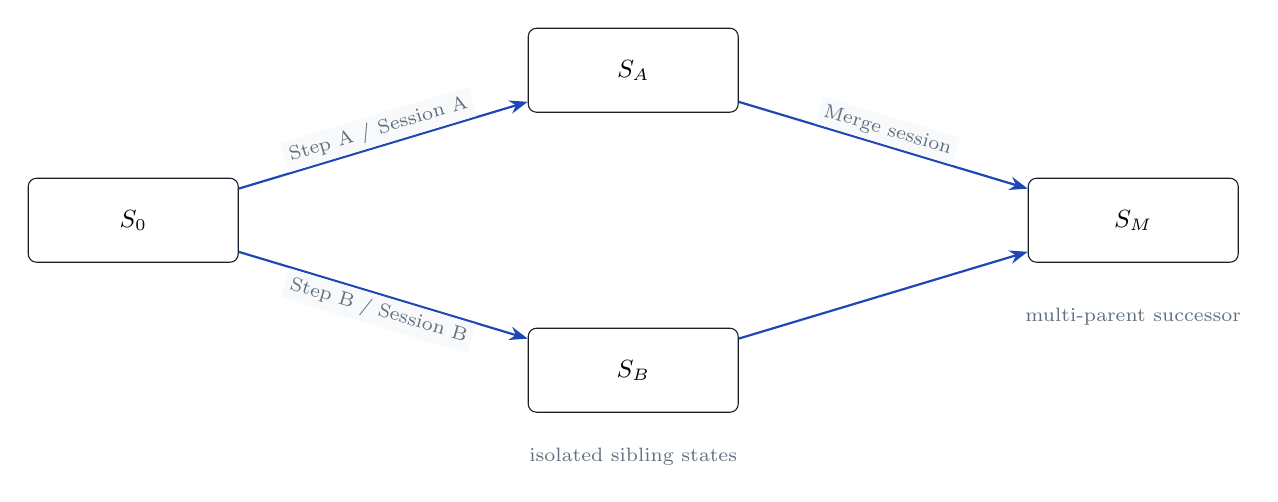
\begin{tikzpicture}[
  state/.style={draw=Ink,fill=white,rounded corners=3pt,minimum width=1.05in,minimum height=0.42in,font=\small\bfseries},
  edgelabel/.style={midway,fill=Paper,inner sep=2pt,font=\scriptsize\color{Muted}},
  edge/.style={-{Stealth[length=2.3mm]},thick,draw=AccentDark}
]
  \node[state] (s0) at (0in,0) {$S_0$};
  \node[state] (sa) at (2.5in,0.75in) {$S_A$};
  \node[state] (sb) at (2.5in,-0.75in) {$S_B$};
  \node[state] (sm) at (5in,0) {$S_M$};
  \draw[edge] (s0) -- node[edgelabel,above,sloped]{Step A / Session A} (sa);
  \draw[edge] (s0) -- node[edgelabel,below,sloped]{Step B / Session B} (sb);
  \draw[edge] (sa) -- node[edgelabel,above,sloped]{Merge session} (sm);
  \draw[edge] (sb) -- (sm);
  \node[font=\scriptsize\color{Muted},align=center] at (2.5in,-1.18in) {isolated sibling states};
  \node[font=\scriptsize\color{Muted},align=center] at (5in,-0.48in) {multi-parent successor};
\end{tikzpicture}
\caption{Concrete execution history. Parallel success creates siblings; combination is an explicit agentic transition.}
\end{figure}

\subsection{Step definitions, instances, and sessions}

A step definition is conceptually

\begin{equation}
 d = (\operatorname{id},\operatorname{revision},\operatorname{instruction},
      \operatorname{harness},\operatorname{model},\operatorname{settings},
      \operatorname{trigger},\operatorname{outputs},\operatorname{bindingSpec}).
\end{equation}

The exact serialized fields are not yet locked. The tuple states the semantic information the design already requires. A step instance \(i\) binds one exact definition revision to an execution context and one session \(q_i\).

\begin{equation}
  \operatorname{SessionOf}(i)=q_i,\qquad
  \operatorname{InstanceOf}(q_i)=i.
\end{equation}

A running session can make many edits, commits, tool calls, and human-visible messages. Those operations remain inside the isolated attempt. They do not each create Playbook states.

\subsection{Trigger-expression grammar}

The selected language is arbitrary Boolean logic, not Horn clauses:

\begin{equation}
\begin{split}
 \phi ::= {} & \operatorname{Exists}(n) \\
        \mid & \operatorname{NewFor}(\mathrm{this\_step},\beta) \\
        \mid & \neg\phi \\
        \mid & (\phi\land\phi) \\
        \mid & (\phi\lor\phi),
\end{split}
\end{equation}

where \(n\) is one exact artifact name and \(\beta\) resolves a complete exact input binding. No arbitrary code, content query, wildcard, type inference, user-defined predicate, rule chaining, or fixed-point inference is implied.

\begin{lstlisting}[style=playbook]
NewFor(this_step, ["implementation.md"])
AND NOT Exists("skip-docs.md")

Exists("approved.md")
OR (
  Exists("needs-revision.md")
  AND NewFor(this_step, ["implementation.md", "needs-revision.md"])
)
\end{lstlisting}

Truth means only: \emph{this configured agentic step should be attempted}. An agent may inspect the full state, determine that it is not semantically adequate, explicitly fail, and publish no successor.

\subsection{Bindings, consumption, and freshness}

For consumer step definition \(d\), a complete input binding \(b\) contains the exact artifact occurrences consumed together. Consumption is not per filename in isolation when the step depends on several inputs.

For successful-transition provenance scope \(\Gamma\), define:

\begin{equation}
\operatorname{ConsumedBy}(d,b,\Gamma)
\iff
\exists \rho\in\Gamma:
  \rho.\operatorname{step}=d
  \land \rho.\operatorname{binding}=b
  \land \rho.\operatorname{outcome}=\mathrm{success}.
\end{equation}

Then:

\begin{equation}
\operatorname{NewFor}(d,b,\Gamma)
\iff
\operatorname{ValidBinding}(d,b)
\land
\neg\operatorname{ConsumedBy}(d,b,\Gamma).
\end{equation}

This makes freshness local to the consumer and the complete binding. Suppose Merge previously consumed \(\{\texttt{tests@2},\texttt{docs@1}\}\). The later binding \(\{\texttt{tests@3},\texttt{docs@1}\}\) is distinct even though the documentation occurrence did not change.

\begin{decisionbox}{TealPale}
\textbf{Single source of truth.} \artifact{ConsumedBy} and \artifact{NewFor} are derived from the immutable provenance already required for the history DAG. Alinery does not maintain a second mutable freshness bit, global consumed flag, cursor, deletion convention, or attempt counter.
\end{decisionbox}

\Open\ The relevant provenance scope \(\Gamma\) is not selected. Ancestry-local scope allows the same binding to be independently consumed on sibling branches; task-global scope lets consumption on one branch suppress another. Exact binding identity and definition-version identity are also open.

\subsection{Applicability and always-live reevaluation}

For a fixed Playbook revision \(P\), state or candidate context \(c\), and resolved binding \(b\):

\begin{equation}
\begin{aligned}
  \operatorname{Applicable}_P(d,c,b) \iff{}&
  d\in P \land \operatorname{BindingValid}(d,c,b) \\
  &{}\land \llbracket d.\operatorname{trigger}\rrbracket_{c,d,b}=\mathsf{true} \\
  &{}\land \operatorname{ActivationEligible}(d,c,b).
\end{aligned}
\end{equation}

The final definition of \(\operatorname{ActivationEligible}\) is open for failed attempts and Boolean expressions without a positive \artifact{NewFor} witness. What is locked is that a new full-state identity alone does not rearm every step.

Whenever a new immutable state is sealed, the Playbook reevaluates every step definition. It does not move a stored program counter or traverse an authored outgoing edge. If several applications are eligible, their sessions may run concurrently.

\subsection{Atomic success, failure, and sealing}

\subsubsection{Success}

A successful session atomically adds exactly one sealed state and one successful provenance record:

\begin{equation}
  (H,\Pi) \xrightarrow{\operatorname{success}(i)}
  (H\cup\{s_i,\operatorname{Parents}(s_i)\to s_i\},
   \Pi\cup\{\rho_i\}).
\end{equation}

All promoted workspace and artifact effects become visible together at this semantic boundary. The agent must explicitly signal completion. Idle, process exit, or mere artifact appearance is insufficient. The completion signal is accepted only after the mechanical output contract is satisfied.

\subsubsection{Failure or semantic rejection}

A failed attempt publishes no state and creates no successful-consumption provenance:

\begin{equation}
  (H,\Pi) \xrightarrow{\operatorname{failure}(i)} (H,\Pi).
\end{equation}

Failure evidence may still be recorded durably outside the successful state DAG; partial workspace changes remain unpromoted and cannot alter the sealed input state.

\subsubsection{Post-completion activity}

After success, the step instance is over and its result is sealed. Even if its PTY process remains alive, subsequent output cannot mutate the sealed state or silently publish a second successor. New state-producing work requires a distinct step instance and session.

\begin{figure}[ht]
\centering
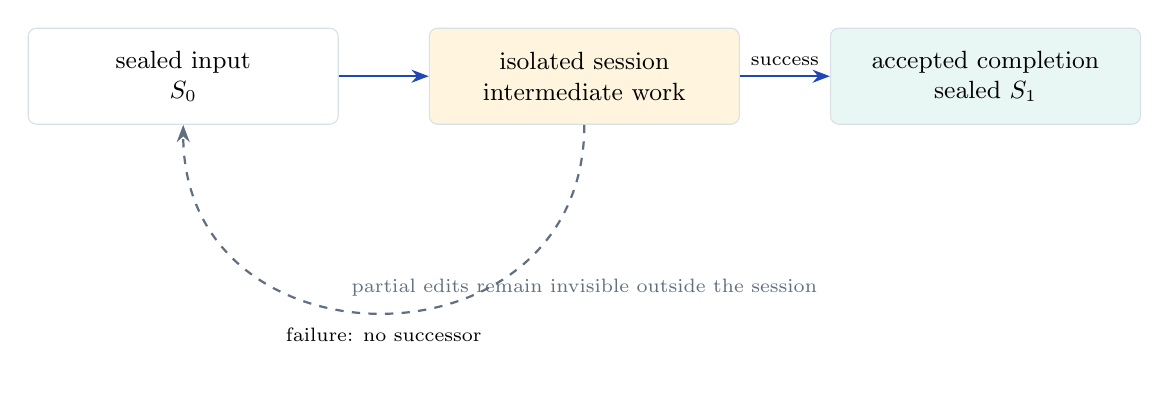
\begin{tikzpicture}[
  box/.style={draw=Rule,fill=white,rounded corners=3pt,minimum width=1.55in,minimum height=0.48in,align=center,font=\small},
  arrow/.style={-{Stealth[length=2.2mm]},thick,draw=AccentDark},
  dashedarrow/.style={-{Stealth[length=2.2mm]},thick,dashed,draw=Muted}
]
  \node[box] (input) at (0in,0) {sealed input\\$S_0$};
  \node[box,fill=AmberPale,right=0.45in of input] (work) {isolated session\\intermediate work};
  \node[box,fill=TealPale,right=0.45in of work] (output) {accepted completion\\sealed $S_1$};
  \draw[arrow] (input) -- (work);
  \draw[arrow] (work) -- node[above,font=\scriptsize]{success} (output);
  \draw[dashedarrow] (work.south) to[out=-90,in=-90,looseness=1.6] node[midway,below=2pt,font=\scriptsize]{failure: no successor} (input.south);
  \node[font=\scriptsize\color{Muted},align=center,below=0.72in of work] {partial edits remain invisible outside the session};
\end{tikzpicture}
\caption{Atomicity is the Playbook visibility boundary. Implementation isolation and cleanup mechanics are still open.}
\end{figure}

\subsection{Concurrent siblings}

If two applicable step instances start from the same sealed state \(s\), each receives an isolated view of \(s\). If both succeed, wall-clock completion order does not make one result a descendant of the other:

\begin{equation}
  s\xrightarrow{A}s_A,\qquad s\xrightarrow{B}s_B,\qquad
  \operatorname{Parents}(s_A)=\operatorname{Parents}(s_B)=\{s\}.
\end{equation}

The results are full, coexisting sibling states. They do not silently merge. This is the chosen answer to parallel work: difficult combination becomes an explicit agent session with human guidance available through its instructions.

\subsection{Agentic merge}

The trigger evaluator decides whether a merge step should start. Once started, the merge agent decides which available states are semantically appropriate to combine, or fails. A successful result records exactly the chosen states as parents.

\begin{equation}
  \operatorname{Select}_m(C_m,K_m)=Q\subseteq C_m
  \quad\text{or}\quad
  \operatorname{Select}_m(C_m,K_m)=\mathsf{fail},
\end{equation}

where \(C_m\) is the candidate set exposed to the merge session and \(K_m\) is the context it can inspect. Neither is yet defined.

\begin{warningbox}[The central unresolved merge tension]
Ordinary atomic steps begin with fixed exact input. The current merge decision says the agent selects exact parents after the merge session starts. The design must still specify the session's initial isolated workspace, whether candidates are frozen at launch, what artifacts witness the trigger, and which binding is consumed if selected parents differ from trigger witnesses.
\end{warningbox}

\section{Process semantics without an authored control graph}

\subsection{No hidden control state}

Given a Playbook and the current immutable material context, Alinery can determine which configured steps should be attempted. The answer must not depend on a stored ``current phase,'' token marking, routing cursor, first-matching edge, or previously traversed graph edge.

Ordering emerges because successful work changes material state and provenance. For example, Design does not follow Research because an edge says so. It follows because its trigger references an exact Research artifact occurrence that Research can produce.

\subsection{Branching and repetition}

If several trigger expressions are true, several steps may run. Mutually exclusive behavior arises only if the relevant predicates are mutually exclusive. A decision agent can write one ordinary named marker:

\begin{lstlisting}[style=playbook]
approved.md
\end{lstlisting}

or:

\begin{lstlisting}[style=playbook]
needs-revision.md
\end{lstlisting}

The engine does not enforce that only one exists. If both exist and both downstream expressions are true, both downstream steps may be attempted. The producing agent's instructions own that semantic discipline in V1.

Repetition arises when a successor contains a distinct binding that makes an earlier step applicable again. No loop object, prefix syntax, version counter, or attempt-count guard is required.

\subsection{Persistent attachment and quiescence}

A Playbook does not close when it runs out of immediate work. It remains attached to the task. Every new immutable state, including a future supported manual state, wakes reevaluation. Quiescence therefore means only ``nothing configured is currently eligible or running.'' It does not certify correctness, completion, or goal achievement.

Immutable history makes future rewind and branching possible without deleting later work. The rewind operation itself is deferred.

\section{Artifacts and decision handoffs}

\subsection{Exact names only}

V1 trigger predicates refer to exact names such as \artifact{design.md}. They do not mean ``a Research document,'' ``the latest file beginning with research-,'' or ``any artifact of type approval.'' This removes implicit selection and keeps the visual and runtime dependency models inspectable.

A logical artifact can retain one stable name across revisions. A successor may overwrite or append to it; immutable ancestor states preserve its earlier values. There is no need to encode the iteration in the filename.

\subsection{Append-only history, mutable current view}

The state history is append-only even when a successor's current view overwrites or removes a named artifact. The old value remains reachable through its ancestor. Therefore preserving inspectability does not require keeping every historical filename simultaneously visible in the current workspace.

\subsection{Outputs and semantic validation}

Successful completion normally requires explicit agent completion plus one or more declared exact named outputs or handoffs. Engine validation should remain mechanical: output identity, presence, regular-file constraints, nonempty requirements where declared, session ownership, and state sealing.

Rich quality checks remain agentic. A Structure step may trigger on a fresh \artifact{design.md}, read it, identify unresolved questions, and fail. This is not a defect in the trigger. The trigger correctly answered whether Structure should inspect the state.

\section{Git-backed persistence direction}

\subsection{Locked direction}

Git is the preferred substrate for complete snapshots, lineage, branching, worktrees, and multi-parent history. Alinery should avoid inventing independent snapshot, diff, restore, merge, and garbage-collection machinery where Git already provides the required mechanics.

Likely mapping:

\begin{itemize}
  \item each task begins on a task branch and usually a worktree;
  \item concurrent attempts use isolated worktrees and sub-branches or equivalent private refs;
  \item successful state publication creates or retains an immutable Git-reachable checkpoint;
  \item a successful agentic merge records multiple selected parents;
  \item non-Git task metadata is included through a versioned manifest or other checkpoint record if required.
\end{itemize}

Only the direction is locked. The exact object/ref strategy is not.

\subsection{History publication}

Detailed checkpoint or commit history is the default. This matches present Alinery behavior, where agent work commonly creates several commits. Squashing remains an optional setting, especially for large Playbooks or final publication. Squashing is not required by the execution model.

Secret-history risk was explicitly placed outside the Playbook engine's V1 scope. Ordinary PR review and remediation remain responsible, as with current agent-authored Git history.

\subsection{Unresolved storage boundary}

\Open\ The following must be selected before implementation:

\begin{itemize}
  \item whether every semantic state is exactly one Git commit;
  \item whether internal commits made during a session are semantic states or hidden implementation detail;
  \item how uncommitted filesystem state is sealed;
  \item how artifacts and non-Git metadata are manifested;
  \item which internal refs keep private objects reachable and garbage-collection safe;
  \item how detailed history is later projected or squashed into ordinary user history.
\end{itemize}

\section{Static definition graph and concrete execution history}

There are two distinct visualizations.

\subsection{Derived Playbook dependency graph}

For step \(d\), let \(\operatorname{Outputs}(d)\) be its declared exact names and \(\operatorname{References}(d)\) the exact names mentioned in \artifact{Exists} or \artifact{NewFor} bindings. A display dependency can be derived:

\begin{equation}
 d_u \leadsto_n d_v
 \iff n \in \operatorname{Outputs}(d_u) \cap \operatorname{References}(d_v).
\end{equation}

This edge is explanatory, not executable order. Because expressions include \texttt{AND}, \texttt{OR}, and \texttt{NOT}, a plain edge list is incomplete. The display must eventually preserve Boolean grouping, negative references, multiple producers, and cycles.

\subsection{Concrete state-history DAG}

The execution view shows actual sealed states, step instances, sessions, exact artifacts, success/failure attempts, and parent lineage. It can be large and is task-specific. Runtime states are never assigned predefined semantic names by the Playbook.

\begin{figure}[ht]
\centering
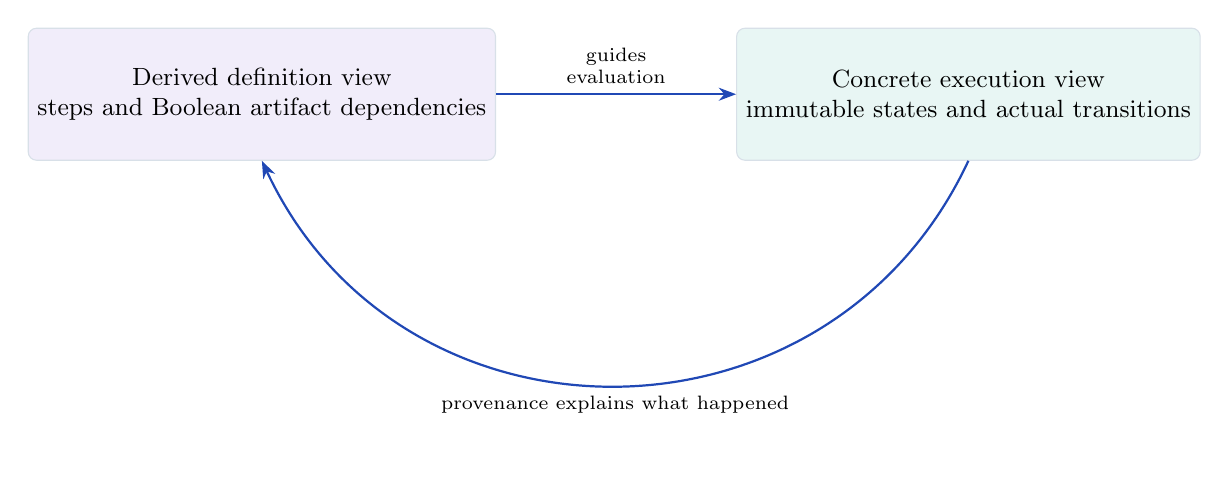
\begin{tikzpicture}[
  box/.style={draw=Rule,rounded corners=3pt,fill=white,minimum width=2.15in,minimum height=0.66in,align=center,font=\small},
  arrow/.style={-{Stealth[length=2.2mm]},thick,draw=AccentDark}
]
  \node[box,fill=PurplePale] (def) at (0in,0) {Derived definition view\\steps and Boolean artifact dependencies};
  \node[box,fill=TealPale,right=1.2in of def] (trace) {Concrete execution view\\immutable states and actual transitions};
  \draw[arrow] (def) -- node[above,font=\scriptsize,align=center]{guides\\evaluation} (trace);
  \draw[arrow] (trace.south) to[out=-115,in=-65,looseness=1.2] node[below,font=\scriptsize]{provenance explains what happened} (def.south);
\end{tikzpicture}
\caption{The visual Playbook graph and one task's state DAG are different projections of the same process.}
\end{figure}

\section{Worked examples}

These examples are semantic test cases, not a settled file syntax.

\subsection{Example A: linear RPI}

\begin{tabularx}{\textwidth}{@{}L{1.15in}L{2.75in}Y@{}}
\toprule
\textbf{Step} & \textbf{Illustrative trigger} & \textbf{Declared output} \\
\midrule
Research & \texttt{NewFor(this, [ticket.md])} & \artifact{research.md} \\
Design & \texttt{NewFor(this, [research.md])} & \artifact{design.md} \\
Structure & \texttt{NewFor(this, [design.md])} & \artifact{plan.md} \\
Implement & \texttt{NewFor(this, [plan.md])} & code changes and \artifact{implementation.md} \\
Validate & \texttt{NewFor(this, [implementation.md])} & \artifact{validation.md} \\
\bottomrule
\end{tabularx}

Successful trace:

\begin{equation}
 S_0 \xrightarrow{\mathrm{Research}} S_1
     \xrightarrow{\mathrm{Design}} S_2
     \xrightarrow{\mathrm{Structure}} S_3
     \xrightarrow{\mathrm{Implement}} S_4
     \xrightarrow{\mathrm{Validate}} S_5.
\end{equation}

The Playbook does not store ``ResearchReady'' or ``DesignReady'' states. Each label belongs to the transition that created the next unnamed material state.

\subsection{Example B: review and revision}

Review examines a fresh implementation and produces exactly one intended marker under its instructions:

\begin{lstlisting}[style=playbook]
Review trigger:
  NewFor(Review, ["implementation.md"])

Revise trigger:
  Exists("needs-revision.md")
  AND NewFor(Revise, ["implementation.md", "needs-revision.md"])

PrepareForPR trigger:
  Exists("approved.md")
  AND NewFor(PrepareForPR, ["implementation.md", "approved.md"])
\end{lstlisting}

If Review requests revision, a distinct Revise session creates a new state and new implementation binding. Review can then become applicable again. The history stays acyclic even though the step label repeats.

\subsection{Example C: conditional documentation}

\begin{lstlisting}[style=playbook]
NewFor(Docs, ["implementation.md"])
AND NOT Exists("skip-docs.md")
\end{lstlisting}

This exercises arbitrary Boolean composition. The predicate is evaluated against the immutable input context. A later concurrent state cannot retroactively change why the Docs session started.

\Open\ An \artifact{Exists}-only or negative-only expression has no obvious positive artifact binding to consume. Its durable activation identity remains unresolved.

\subsection{Example D: parallel specialists and synthesis}

Security Research and UX Research are both applicable at \(S_0\). They receive isolated views and complete independently:

\begin{align}
 S_0 &\xrightarrow{\mathrm{SecurityResearch}} S_A,\\
 S_0 &\xrightarrow{\mathrm{UXResearch}} S_B.
\end{align}

Neither state contains the other's partial work. Synthesis is an agentic merge. It inspects candidate lineage, selects appropriate parents, reconciles their work, and either publishes

\begin{equation}
 \operatorname{Parents}(S_M)=\{S_A,S_B\}
\end{equation}

or fails with no successor.

This example exposes the unresolved evaluation scope: no individual sibling necessarily contains both specialist artifacts, so multi-state \artifact{Exists}/\artifact{NewFor} semantics and candidate construction must be defined.

\subsection{Example E: corrected revision before synthesis}

The following is \textbf{not} allowed:

\begin{equation}
 S_0 \xrightarrow{A/\mathrm{session}\ A_1} S_{A1}
 \quad\text{and later the same completed session silently emits }S_{A2}.
\end{equation}

Atomic completion sealed \(S_{A1}\). A later revision requires a distinct transition:

\begin{equation}
 S_{A1}\xrightarrow{\mathrm{ReviseA}/\mathrm{new\ session}}S_{A2}.
\end{equation}

Only an explicit new step instance, manual state-producing operation, or separately valid activation can create \(S_{A2}\). If several candidate versions remain live before synthesis, the merge agent's visible candidate set and selection protocol are still open.

\subsection{Example F: mechanically triggered, semantically rejected}

Structure triggers because a fresh \artifact{design.md} exists. Its agent reads the document and discovers unresolved design questions. It explicitly fails. The attempt is recorded, no successor state is published, and no successful consumption provenance is created.

This behavior is intentional. The trigger is a dispatch rule, not a semantic theorem prover.

\subsection{Example G: human approval inside a step}

The Design agent is instructed to consult a human and withhold completion until approval. The running session, dirty isolated workspace, and conversation remain inside one atomic step. After approval and accepted completion, one successor is sealed.

A standalone human-only step is deferred. A human comment made after the session is sealed cannot change the completed state through that old session; the interaction mechanism is the paused open question.

\subsection{Example H: manual work after quiescence}

The Playbook becomes quiescent. Later, a supported manual operation creates a new immutable state with a changed relevant artifact. The Playbook remains attached, wakes, and reevaluates all triggers. Only newly eligible bindings may run; a new state identifier alone does not refresh old inputs.

\Open\ The exact operation that captures and seals manual filesystem edits is not yet designed.

\section{Current Alinery baseline and replacement delta}

This section is descriptive evidence from repository commit \baselinehash. It is not a claim that the current implementation already satisfies the proposed model.

\subsection{Current verified behavior}

\begin{itemize}
  \item The current schema types are \texttt{WorkflowFile}, \texttt{Workflow}, \texttt{WorkflowStep}, and \texttt{AutoAdvanceEdge}. They are defined in \path{alinery-core/src/types.rs}.
  \item Repository-owned \texttt{.alinery/workflows.toml} is parsed and cached by modification time, with bundled defaults.
  \item Current auto-advance is represented by named \texttt{from}/\texttt{to} edges. The task selects edge keys.
  \item \texttt{find\_enabled\_auto\_edge} returns the first selected edge whose \texttt{from} equals the completed phase, so the current runtime creates at most one next phase for a source.
  \item Completion requires an explicit accepted \texttt{alinery\_phase\_complete} event and validation of the expected nonempty regular artifact. Idle, end of turn, and process exit are not completion.
  \item Auto-advance uses a deterministic target session identifier and exclusive metadata creation to prevent duplicate target sessions across daemons.
  \item Current task execution uses a task worktree and phase/session metadata, not immutable full-state siblings and multi-parent transitions.
  \item Bundled definitions include RPI, One-shot, Free-form, Review, and Bug Hunting.
\end{itemize}

\subsection{Replacement delta}

\begin{longtable}{@{}L{1.35in}L{2.35in}L{2.80in}@{}}
\toprule
\textbf{Concern} & \textbf{Current workflow behavior} & \textbf{Selected Playbook model} \\
\midrule
\endfirsthead
\toprule
\textbf{Concern} & \textbf{Current workflow behavior} & \textbf{Selected Playbook model} \\
\midrule
\endhead
Terminology & Workflow, phase, auto-advance edge & Playbook, step definition/instance, trigger expression, state transition \\
Ordering & Authored \texttt{from}/\texttt{to} edges & Derived from state predicates, exact outputs, and provenance \\
Branching & One selected outgoing edge for a completed phase & Every independently applicable step may run \\
State & One task worktree plus session/phase metadata & Immutable complete task states with explicit lineage \\
Concurrency & Not a full sibling-state semantic model & Isolated sessions from the same parent yield siblings \\
Merge & No general multi-parent agent step & Explicit agentic step selects parents or fails \\
Repetition & Target phase deduplicated as a one-time session & Repeated definition instances over distinct bindings; no loop object \\
Freshness & Phase/session identity and target existence & Per-consumer complete binding derived from provenance \\
Completion & Explicit phase-complete plus expected artifact & Preserve explicit completion; generalize mechanical output contract \\
Graph & Authored edge graph & Derived dependency view plus concrete history DAG \\
Lifetime & Primary workflow progression & Persistently attached reactive process \\
\bottomrule
\end{longtable}

\subsection{Current issue scope that should remain unless explicitly revised}

The live DEL-603 epic additionally requires file loading and validation shared across app, daemon, and MCP; actionable parse errors rather than silent fallback; Settings to manage Playbooks; raw and form editing; registered-harness authorization; Generic sessions without a Playbook; per-step harness/model guidance; custom board projection; and an agentic Playbook Builder that writes a candidate file for explicit review and installation.

The physical choice between one portable Markdown/YAML-style file and the existing registry plus external Markdown prompts remains open. The epic explicitly says not to add a second parser until the chosen form requires it.

\section{Conceptual data contract, not serialized schema}

The following records are the minimum conceptual information implied by locked semantics. Field names and serialization are deliberately provisional.

\begin{lstlisting}[style=playbook]
PlaybookRevision {
  playbook_id
  revision_id
  metadata
  step_definitions[]
}

StepDefinitionRevision {
  step_id
  revision_id
  prompt_or_instruction
  harness
  model
  harness_settings
  trigger_expression
  binding_specification
  declared_outputs[]
  completion_contract
}

TaskState {
  state_id
  parent_state_ids[]
  snapshot_reference
  artifact_manifest
  creating_transition_id
  optional_title = ""
}

StepAttempt {
  attempt_id
  step_definition_revision_id
  session_id
  evaluation_context
  proposed_or_resolved_binding
  status
  failure_reason?
}

SuccessfulTransitionProvenance {
  transition_id
  step_definition_revision_id
  session_id
  exact_parent_state_ids[]
  exact_input_binding
  exact_outputs
  result_state_id
  accepted_completion
}
\end{lstlisting}

\begin{warningbox}[Do not freeze these fields by implementation accident]
The conceptual records expose information the semantics require. They do not decide the Playbook file syntax, state storage layout, Git mapping, failure-suppression key, merge parent protocol, or client-server wire representation.
\end{warningbox}

\section{Runtime invariants and acceptance properties}

Any implementation proposal should be rejected if it cannot demonstrate these locked or directly derived properties.

\begin{longtable}{@{}L{0.52in}L{0.88in}L{5.10in}@{}}
\toprule
\textbf{ID} & \textbf{Status} & \textbf{Invariant} \\
\midrule
\endfirsthead
\toprule
\textbf{ID} & \textbf{Status} & \textbf{Invariant} \\
\midrule
\endhead
I-01 & \Locked & Every sealed task state is immutable and independently inspectable. \\
I-02 & \Locked & Every successful ordinary step instance has exactly one parent and at most one successor. \\
I-03 & \Locked & Every successful merge records every and only the exact parent states chosen by its merge agent. \\
I-04 & \Locked & One step instance corresponds to exactly one session; one session cannot represent two step instances. \\
I-05 & \Locked & Intermediate session mutations are not Playbook states and are withheld from trigger evaluation. \\
I-06 & \Locked & Failure or semantic rejection creates no successor state. \\
I-07 & \Derived & Failed partial filesystem changes cannot leak into or rewrite the sealed input state. \\
I-08 & \Locked & Idle, process exit, or end of turn alone cannot complete a step. \\
I-09 & \Locked & Successful completion requires an explicit agent completion signal accepted by Alinery. \\
I-10 & \Locked & Trigger truth means ``attempt,'' not ``guaranteed success.'' \\
I-11 & \Locked & Concurrent successful instances from the same parent produce sibling states, regardless of wall-clock finish order. \\
I-12 & \Locked & Concurrent results never combine without an explicit successful merge transition. \\
I-13 & \Locked & A completed session cannot mutate its sealed result or publish another successor. \\
I-14 & \Locked & The evaluator uses no hidden control cursor, authored ordering edge, gateway, or first-match rule. \\
I-15 & \Locked & Every applicable step may run; concurrency follows from independent trigger truth. \\
I-16 & \Locked & Trigger predicates reference only exact named artifacts and provenance-derived binding freshness. \\
I-17 & \Locked & Consumption is per consumer and complete input binding. \\
I-18 & \Locked & \artifact{ConsumedBy} and \artifact{NewFor} have immutable provenance as their sole source of truth. \\
I-19 & \Locked & Unrelated state identity changes do not automatically refresh an unchanged binding. \\
I-20 & \Locked & The Playbook remains attached and reevaluates after every newly sealed state. \\
I-21 & \Locked & Quiescence is not represented as task success or goal satisfaction. \\
I-22 & \Locked & Runtime states have no predefined semantic names or Playbook control identity. \\
I-23 & \Locked & Repetition creates new immutable states and step instances; no state-history cycle or loop counter is required. \\
I-24 & \Locked & Decision-marker exclusivity is not engine-enforced in V1. \\
I-25 & \Derived & The concrete state history is a DAG even when the derived Playbook dependency view contains cycles. \\
\bottomrule
\end{longtable}

\section{Exhaustive decision ledger}

This ledger condenses the chronological elicitation into implementation-reviewable decisions. It intentionally includes rejections so future design work does not reopen them accidentally.

\begin{longtable}{@{}L{0.52in}L{0.88in}L{5.10in}@{}}
\toprule
\textbf{ID} & \textbf{Status} & \textbf{Decision or boundary} \\
\midrule
\endfirsthead
\toprule
\textbf{ID} & \textbf{Status} & \textbf{Decision or boundary} \\
\midrule
\endhead
D-001 & \Locked & Use ``Playbook'' as the product term replacing ``workflow.'' \\
D-002 & \Locked & A Playbook is a preconfigured team/process of agent sessions. \\
D-003 & \Locked & Optimize for powerful customization and a simple, inspectable human mental model. \\
D-004 & \Rejected & No runtime planning search, goal solving, POMDP model, or arbitrary code control language in V1. \\
D-005 & \Locked & A state is the complete material task state, not a session or lifecycle label. \\
D-006 & \Locked & States are immutable complete versions with lineage and remain independently addressable. \\
D-007 & \Locked & States have no hidden control position or predefined semantic name. \\
D-008 & \Deferred & Optional state title/description may come later with no V1 semantics. \\
D-009 & \Locked & A step is a transition specification between states. \\
D-010 & \Locked & A step definition includes prompt/instructions, harness, model, settings, trigger, and exact outputs. \\
D-011 & \Locked & One step instance is executed by one PTY harness session, one-to-one. \\
D-012 & \Locked & A step is atomic at the Playbook visibility boundary. \\
D-013 & \Locked & Running-session edits remain withheld until the complete contract succeeds. \\
D-014 & \Locked & Failure produces no successor and preserves the sealed input. \\
D-015 & \Open & Failed workspace cleanup and durable retry suppression are not specified. \\
D-016 & \Locked & A completed session cannot later change its result or emit a second result state. \\
D-017 & \Locked & Several independently applicable steps may run concurrently. \\
D-018 & \Locked & Concurrent instances receive isolated views of the same input and produce full sibling states. \\
D-019 & \Rejected & Concurrent sessions do not directly mutate one shared output state. \\
D-020 & \Locked & Combination requires an explicit agentic merge step. \\
D-021 & \Locked & A successful merge result records all chosen parents, producing a traceable DAG. \\
D-022 & \Open & The current active frontier and merge candidate-set construction remain undefined. \\
D-023 & \Locked & Git is the preferred lineage/snapshot substrate; avoid custom snapshot/diff/merge/GC machinery where possible. \\
D-024 & \Open & Exact Git checkpoint, private-ref, manifest, and uncommitted-state mapping remain unresolved. \\
D-025 & \Locked & Detailed commit/checkpoint history is default; squashing is optional. \\
D-026 & \Rejected & Secret-history policy is not added to the Playbook engine's V1 responsibilities. \\
D-027 & \Locked & Idle or process exit never completes a step. \\
D-028 & \Locked & The agent explicitly requests completion; mechanical declared outputs are validated. \\
D-029 & \Rejected & No rich engine-enforced semantic postconditions in V1. \\
D-030 & \Locked & Agents may reject mechanically eligible states and fail without successors. \\
D-031 & \Locked & Human approval may occur inside an agent step before atomic completion. \\
D-032 & \Rejected & Standalone human-only steps are excluded from V1. \\
D-033 & \Locked & Manual and Generic work outside the configured Playbook remains possible. \\
D-034 & \Open & Human interaction with completed sessions is paused for later examples. \\
D-035 & \Rejected & No explicit authored ordering edges or routing objects in the selected model. \\
D-036 & \Locked & Given the Playbook and immutable state/context, trigger expressions determine applicable work. \\
D-037 & \Locked & If several triggers are true, several steps may run; no split/gateway construct is required. \\
D-038 & \Locked & The displayed graph is derived from predicates and declared outputs, not an execution source of truth. \\
D-039 & \Locked & A loop is repeated state-based applicability, not a first-class object or counter. \\
D-040 & \Locked & V1 predicates reference exact named artifacts only. \\
D-041 & \Rejected & No semantic artifact types, prefixes, wildcards, or implicit latest-version lookup. \\
D-042 & \Locked & Stable artifact names may be overwritten/appended in successors; immutable history preserves prior values. \\
D-043 & \Rejected & Do not delete an artifact merely to mark it consumed. \\
D-044 & \Rejected & No global freshness, global consumed bit, mutable cursor, or separate consumption source of truth. \\
D-045 & \Locked & Consumption is per consumer and complete exact binding. \\
D-046 & \Locked & \artifact{ConsumedBy} and \artifact{NewFor} are derived from immutable transition provenance. \\
D-047 & \Open & Exact artifact occurrence, binding identity, and provenance scope remain undefined. \\
D-048 & \Locked & Decision agents communicate through ordinary exact named marker artifacts. \\
D-049 & \Locked & Agent instructions, not the V1 engine, own marker exclusivity. \\
D-050 & \Derived & If conflicting markers coexist and both triggers are true, both steps may be attempted. \\
D-051 & \Rejected & A step trigger is not limited to one flat conjunction or to Horn clauses. \\
D-052 & \Locked & Trigger expressions allow arbitrary \texttt{AND}, \texttt{OR}, and \texttt{NOT} over \artifact{Exists} and \artifact{NewFor}. \\
D-053 & \Locked & Trigger truth means ``should attempt,'' never ``will succeed.'' \\
D-054 & \Open & Boolean witness/binding semantics for \texttt{OR}, negative predicates, and \artifact{Exists}-only triggers remain unresolved. \\
D-055 & \Locked & The Playbook stays live and attached after quiescence. \\
D-056 & \Locked & Every newly sealed state wakes reevaluation of all step definitions. \\
D-057 & \Rejected & A new full-state identity alone does not rearm all true steps. \\
D-058 & \Locked & Quiescence is a process condition, not a goal or success proof. \\
D-059 & \Deferred & Rewind should be enabled by history later but is not in the current design scope. \\
D-060 & \Locked & The merge trigger decides when to start; the merge agent decides exact parents or fails. \\
D-061 & \Open & Merge session context, trigger witnesses, launch snapshot, candidate freezing, and parent declaration protocol remain undefined. \\
D-062 & \Locked & Same-session post-completion activity cannot explain a second state; a separate transition is required. \\
D-063 & \Deferred & The specific UX for creating that new manual transition is not decided. \\
D-064 & \Locked & Playbooks are file-based and should be authorable by an ordinary agent session. \\
D-065 & \Open & Single portable file versus registry plus prompt files, and the final Boolean AST syntax, remain design work. \\
D-066 & \Current & DEL-603 requires shared validation, actionable errors, builder/management UI, registered harnesses, and Generic sessions. \\
D-067 & \Current & Current auto-advance uses selected \texttt{from}/\texttt{to} edges and one next phase, not the selected state model. \\
D-068 & \Open & Playbook revision identity and its effect on old consumption and always-live reevaluation remain undefined. \\
D-069 & \Open & External side effects outside the isolated filesystem are not covered by atomic state rollback. \\
D-070 & \Open & Crash recovery, exactly-once attempt claiming, resource limits, and scheduling fairness require implementation design after semantics settle. \\
\bottomrule
\end{longtable}

\section{Rejected and deferred models}

\subsection{Explicitly rejected}

\begin{itemize}
  \item Session as state; step as state; named phase as concrete task state.
  \item Required named checkpoints or semantic state nodes.
  \item Hidden control cursor, stored routing state, authored ordering edges, first-match routing, gateways, splits, or routing tokens.
  \item First-class loops, loop identity, loop counters, or attempt-count predicates as core control.
  \item Runtime goal expressions, plan synthesis, search, or partially observable decision models.
  \item Arbitrary executable trigger code, semantic artifact queries, prefixes, wildcard matching, or implicit artifact types.
  \item Global freshness, global consumption, deletion-as-consumption, separate mutable consumption records, or counters.
  \item Trigger truth as semantic validity or success proof.
  \item Rich engine-enforced semantic postconditions.
  \item Silent combination of concurrent changes.
  \item Same completed session producing several successor states.
  \item Human-only steps in V1.
  \item Required squashing as default history behavior.
\end{itemize}

\subsection{Explicitly deferred}

\begin{itemize}
  \item First-class human-only steps, regulatory approvals, signatures, and role authorization.
  \item Human interaction with completed sessions and automatic versus explicit follow-up transitions.
  \item Rewind UI and operations.
  \item Optional state titles/descriptions.
  \item Goal-directed planning and dynamic Playbooks.
  \item Engine-enforced marker exclusivity.
  \item Hosted community marketplace, ratings, moderation, and publishing after the local format stabilizes.
\end{itemize}

\section{Open decision frontier}

The following are real semantic questions. They must remain visibly open rather than being answered by an implementation shortcut.

\subsection{Human interaction}

\begin{enumerate}
  \item If a human messages a completed session, is it read-only until an explicit new session is created, or does the UI create a new manual step instance?
  \item What event atomically captures manual filesystem edits as a new state?
  \item How is post-completion approval reversal or correction represented while human-only steps remain deferred?
\end{enumerate}

\subsection{Merge candidate and parent semantics}

\begin{enumerate}
  \item Which states, artifacts, and lineage are exposed to a triggered merge session: every live branch head, only trigger witnesses, or another derived candidate set?
  \item Is the candidate set frozen when the session starts? May the agent select a state produced while it is running?
  \item Which isolated workspace does a merge session initially receive before choosing parents?
  \item How does the agent declare exact parents and how does Alinery validate them?
  \item Does a failed merge reject one candidate binding or the whole visible candidate set?
  \item What happens to unchosen live alternatives after success?
\end{enumerate}

\subsection{Boolean binding semantics}

\begin{enumerate}
  \item Consider \texttt{NewFor(A) OR NewFor(B)}. When both are new, is there one binding, two bindings, or an expression-witness binding?
  \item What durable activation identity suppresses repeated \texttt{Exists(A)} or \texttt{NOT Exists(A)} attempts when unrelated states appear?
  \item What does \texttt{NOT NewFor(A)} mean when absence and prior consumption can both make \artifact{NewFor} false?
  \item Is \artifact{ConsumedBy} evaluated over ancestry, a branch, the active frontier, or all task provenance?
  \item Does changing a Playbook or step-definition revision make an old material binding new for the revised consumer?
\end{enumerate}

\subsection{Failure and retry}

\begin{enumerate}
  \item How is a failed but still mechanically applicable binding prevented from auto-retrying forever?
  \item How does explicit retry override that suppression without falsely recording successful consumption?
  \item Are crash, cancellation, semantic rejection, and infrastructure failure distinct attempt outcomes for retry policy?
\end{enumerate}

\subsection{State frontier and manual creation}

\begin{enumerate}
  \item What exact set of immutable states is currently live when several branches coexist?
  \item How do branch heads or refs move after ordinary successors and merges?
  \item Can ancestor and descendant states both remain live candidates?
  \item Which manual operations create states, and can a manual state have multiple parents?
\end{enumerate}

\subsection{Storage, recovery, and Playbook evolution}

\begin{enumerate}
  \item Must every semantic state be a Git commit? How are uncommitted and non-Git data sealed?
  \item What keeps internal Git objects reachable and garbage-collection safe?
  \item What exact Playbook/step revision is captured by a running step instance?
  \item Do Playbook edits immediately reevaluate existing live states or wait for the next state event?
  \item How are state publication, provenance persistence, and attempt claiming recovered exactly once across crashes?
  \item What scheduler capacity and fairness policy limits simultaneous applicable steps without changing their logical applicability?
\end{enumerate}

\subsection{Serialization and display}

\begin{enumerate}
  \item What is the portable file format and Boolean-expression AST?
  \item How are prompts embedded or referenced while preserving one-file portability where desired?
  \item How does the builder explain \texttt{AND}/\texttt{OR}/\texttt{NOT}, negative dependencies, and merge candidate requirements?
  \item How are the derived definition graph and concrete state DAG presented without conflating them?
\end{enumerate}

\section{Implementation gates after design completion}

These are not implementation instructions yet. They are evidence the eventual design must make testable.

\begin{enumerate}
  \item A validated Playbook revision produces the same trigger AST in app, daemon, and MCP consumers.
  \item Trigger evaluation is deterministic for a fixed Playbook revision, state/candidate context, binding, and provenance scope.
  \item At most one live attempt may claim the same activation key, including across daemon crashes or competitors.
  \item No partial session edit changes a sealed state or becomes visible to another isolated sibling.
  \item Accepted success persists result state, parent edges, and provenance atomically or recovers to one consistent outcome.
  \item Failure persists enough attempt evidence to explain and suppress uncontrolled retries while adding no successor state.
  \item A merge cannot claim a parent it was not authorized to inspect and did not declare.
  \item Graph rendering is derived from the same parsed trigger/output model used by execution.
  \item Invalid Playbooks cannot start sessions and never silently fall back to a different definition.
  \item Built-in RPI, Review/revision, Boolean conditional, parallel sibling, merge, failure, manual wake, and post-completion cases are executable conformance traces.
\end{enumerate}

\section{Literature alignment, without importing its control model}

The selected design uses familiar concepts but is not a direct implementation of any one formalism.

\begin{itemize}
  \item Classical planning gives precise vocabulary for state, action applicability, and successor transitions, but this Playbook does not search for a plan or declare a goal \cite{strips}.
  \item The concrete material state is unbounded because repositories and artifacts are unbounded. ``Labelled transition system'' or ``extended state machine'' is more technically accurate than a literal finite-state machine. The product can still visualize finite definitions and finite execution traces \cite{statecharts}.
  \item Long-running harness sessions reinforce the distinction between the duration of execution and the atomic before/after boundary used for Playbook semantics \cite{pddl21}.
  \item PDDL derived predicates use restricted rule semantics and fixed-point evaluation. The selected arbitrary Boolean \artifact{Exists}/\artifact{NewFor} expression language is simpler direct evaluation and should not be called Horn clauses or a derived-predicate engine \cite{pddl22,axioms}.
  \item Git natively represents immutable trees, commits with parents, branches/refs, and merge commits. The exact mapping remains a storage decision, but Git is the preferred substrate rather than a model Alinery should reimplement \cite{gitcommit,gitglossary}.
\end{itemize}

These citations clarify terminology. They do not override product decisions, add control tokens, or imply runtime planning.

\clearpage
\section{Design session continuation: explicit lineage and state publication}

\begin{summarybox}[Status of this append]
This section records the design decisions made after the original checkpoint, through question 47. It is intentionally additive: earlier sections have not been reorganized or reconciled. Where an earlier open question conflicts with a locked statement here, this later section is authoritative. Questions explicitly marked open below remain unresolved.
\end{summarybox}

\subsection{Independent states, not an active frontier}

Every sealed task state remains an immutable, independently valid object. Creating a descendant does not supersede, deactivate, consume, or make its ancestors stale. The V1 model has no active branch, stale branch, stale artifact, leaf-state restriction, or stored frontier. A ``branch'' is only a path that can be derived from the recorded state DAG.

Ordinary step applicability remains state-local. A session started from \(S_A\) receives \(S_A\); it does not implicitly see artifacts that exist only in sibling \(S_B\). If a Playbook trigger is applicable to several independent states, each state may support an independent step instance. Existing states remain available for later inspection and future transitions.

\begin{decisionbox}{TealPale}
\textbf{No supersession rule.} Lineage explains how states were produced. It does not select one current truth and does not prune older states from the execution model.
\end{decisionbox}

\subsection{Human-created continuations are ordinary branches}

Questions and conversation may occur at any time without creating a state. If a human asks an agent to perform material work from a sealed state, that work requires a distinct step instance and session rooted at the selected state. Intermediate edits remain isolated. Accepted success seals one new child; failure seals none.

The original state and the human-created child then coexist. The UI should expose this continuation as another visible branch of the history. The Playbook evaluates the new state normally while every other independent state remains valid and independently eligible. No branch is activated or deactivated as a side effect of this interaction.

\subsection{Cross-state merge and exact parent selection}

Merge is the cross-state exception to ordinary state-local evaluation. Its precondition can search the recorded immutable states for the exact named outputs it requires. Candidate states are the states that can supply those qualifying outputs, wherever they occur in history. Requiring candidates to be leaves would add an unrelated control concept and is rejected.

One configured Synthesis step may succeed from one parent when one state contains all required material, or from several parents when the required material is distributed. ``Merge'' describes the multi-parent execution case, not a separate authored split, gateway, or routing node.

The candidate set is context, not lineage. The merge session inspects the available candidates and, on completion, declares the exact subset it actually selected. Only that validated subset becomes the parent set of its successor:

\begin{equation}
  Q_m \subseteq C_m,
  \qquad
  \operatorname{Parents}(S_m)=Q_m.
\end{equation}

Alinery cannot infer \(Q_m\) from every state the agent opened, read, or considered, because inspection does not imply selection. If semantic combination is unclear, the merge agent may ask the human for clarification inside the same still-running atomic session. Playbook instructions should tell it when and how to do so. That conversation and any intermediate work publish no state. The session eventually declares a parent subset and completes, or fails.

The exact mechanism for delivering and freezing merge candidates remains implementation work. The settled requirement is that candidate discovery is not restricted to an active or leaf frontier and exact selected parents are declared at accepted completion.

\subsection{The state DAG is explicit persisted data}

Playbooks must persist their concrete state DAG directly. Parentage is not reconstructed later from Git history, artifact coincidence, session ordering, or which files an agent happened to inspect.

\begin{itemize}
  \item A genesis state records \texttt{parent\_state\_ids: []}.
  \item For an ordinary execution started from \(S_0\), Alinery already knows the execution context and records \texttt{parent\_state\_ids: [S0]}.
  \item For a human-created continuation, Alinery records the sealed state selected when that continuation started.
  \item For a merge, the agent declares its chosen subset at completion; Alinery validates and records exactly those state identifiers.
\end{itemize}

\begin{warningbox}[Current implementation gap]
Current Alinery workflows do not persist this model. They have task metadata, session metadata, a task worktree, mutable artifacts, and a small accepted phase-completion checkpoint. They do not have immutable task-state identifiers, explicit parent arrays, artifact-version identities, exact successful input bindings, or a persisted state DAG. The present \texttt{alinery\_phase\_complete} path advances workflow/session metadata; it does not publish an immutable task-state manifest.
\end{warningbox}

\subsection{One immutable manifest per successful state}

The minimum durable representation is one engine-generated immutable manifest for every successfully sealed state. The manifest is published when Alinery accepts an explicit step-completion signal, not when a harness exits, becomes idle, stops producing output, or merely writes an artifact. In Playbook terminology, \texttt{step\_complete} generalizes the current phase-completion event.

The sealing sequence is:

\begin{enumerate}
  \item Alinery starts an isolated step instance and retains its engine-known context: session identifier, exact step-definition revision, and ordinary parent state. A merge additionally receives candidate-state context.
  \item The agent and any participating human perform work inside the session. Code, artifacts, commits, dirty filesystem changes, and conversation remain intermediate and create no Playbook state.
  \item The agent emits the explicit completion signal. A merge supplies its selected parent-state identifiers with that structured signal.
  \item Alinery prevents a second publication for the same attempt, validates the mechanical output contract, and validates any merge-parent selection against the session's authorized candidates.
  \item Alinery creates the internal Git checkpoint that captures committed and dirty work and snapshots or hashes the visible artifact versions. The exact Git object and ref layout remains a storage decision.
  \item Alinery generates the state identifier and authoritative manifest fields, then writes the complete manifest atomically.
  \item Publication of that manifest is the state-creation commit point. Only afterward does Alinery record accepted success and reevaluate the attached Playbook against the new state.
\end{enumerate}

If validation, checkpointing, artifact capture, or manifest publication fails, no successor state exists and no successful provenance is recorded. A completed session cannot later mutate its sealed result. Further material work requires another step instance and, on success, another manifest.

\subsection{The engine owns the manifest}

The agent must not write or edit the authoritative manifest. Prompts may explain the completion contract and provide candidate state identifiers, but prefilled bookkeeping is not authoritative provenance. Otherwise lineage correctness would depend on an agent copying engine facts without error.

Alinery mechanically supplies:

\begin{itemize}
  \item the new state identifier;
  \item exact parent-state identifiers, using the launch parent for ordinary work and the validated selected subset for merge;
  \item session and step-definition revision identifiers;
  \item the Git checkpoint or equivalent snapshot reference;
  \item exact artifact-version identities and declared outputs;
  \item the resolved exact input binding;
  \item the accepted completion timestamp and transition outcome.
\end{itemize}

The agent supplies only facts that require its semantic judgment: the actual code and artifact contents, the explicit completion signal, and, for a merge, \texttt{selected\_parent\_state\_ids}. For V1, every successful state has exactly one creating transition, so the transition provenance can live in the same immutable manifest. A separate successful-transition database is not required by the selected semantics.

\Needspace{3.6in}
The following is a conceptual example, not a locked serialized schema:

\begin{lstlisting}[style=playbook]
TaskStateManifest {
  state_id: "S18"
  parent_state_ids: ["S15", "S17"]

  snapshot: {
    git_checkpoint: "3f4c..."
  }

  artifacts: {
    "security.md": "artifact-version-91"
    "ux.md":       "artifact-version-104"
  }

  created_by: {
    session_id: "session-42"
    step_definition_revision_id: "synthesis@7"
    resolved_input_binding: {
      "security.md": "artifact-version-91"
      "ux.md":       "artifact-version-104"
    }
    declared_outputs: ["implementation-plan.md"]
    accepted_completion_at: "..."
  }
}
\end{lstlisting}

\subsection{Derived consumption and freshness}

The manifest makes successful transition provenance concrete. It does not add mutable \texttt{consumed} or \texttt{fresh} fields. Given step-definition revision \(d\) and exact resolved binding \(b\):

\begin{equation}
\begin{aligned}
  \operatorname{ConsumedBy}(d,b)
  \iff{}& \text{an immutable successful state manifest records}\\
         & \text{creating step revision }d\text{ with exact binding }b,\\[0.4em]
  \operatorname{NewFor}(d,b)
  \iff{}& \operatorname{ValidBinding}(d,b)
  \land \neg\operatorname{ConsumedBy}(d,b).
\end{aligned}
\end{equation}

Thus the state DAG and its embedded successful provenance are explicit persisted facts; \artifact{ConsumedBy} and \artifact{NewFor} are queries derived from those facts. Exposing a candidate to a merge, inspecting a state, or starting a failed attempt does not itself write successful-consumption provenance.

\begin{warningbox}[Still open: binding and \artifact{NewFor} surface]
The design has not selected where an ordinary step's exact input binding comes from. It may be a separately declared input field, the artifact references inside \artifact{NewFor}, or another mechanically resolved specification. The design also has not selected whether authors place \artifact{NewFor} explicitly in trigger expressions or whether Alinery automatically enforces one successful execution per exact binding while exposing \artifact{NewFor}/\artifact{ConsumedBy} only as derived engine and UI concepts. Boolean witness semantics, provenance scope, and step-revision effects remain open as recorded earlier. No file schema should silently answer these questions.
\end{warningbox}

\subsection{Append-only decision ledger for this continuation}

\begin{longtable}{@{}L{0.52in}L{0.88in}L{5.10in}@{}}
\toprule
\textbf{ID} & \textbf{Status} & \textbf{Decision or boundary} \\
\midrule
\endfirsthead
\toprule
\textbf{ID} & \textbf{Status} & \textbf{Decision or boundary} \\
\midrule
\endhead
D-071 & \Locked & Every immutable state remains independently valid; there is no active, stale, leaf-only, or stored frontier semantics. \\
D-072 & \Locked & Material human-requested follow-up runs as a distinct session from a selected sealed state and may produce an ordinary coexisting child. \\
D-073 & \Locked & Merge candidate discovery may search all recorded states for required exact named outputs; it is not leaf-restricted. \\
D-074 & \Locked & One step definition may complete with one parent or several, depending on where its selected inputs reside. \\
D-075 & \Locked & A merge agent declares the exact chosen parent subset at completion; inspection and candidate exposure do not define parentage. \\
D-076 & \Locked & A merge agent may seek human clarification inside its still-running atomic session, as guided by its Playbook prompt. \\
D-077 & \Locked & Every successful state records its parent identifiers explicitly; the task-state history DAG is persisted, not reconstructed. \\
D-078 & \Locked & Accepted explicit completion publishes exactly one immutable engine-generated state manifest; failure publishes none. \\
D-079 & \Locked & Alinery owns state identifiers, parent validation, checkpoint and artifact capture, provenance, and atomic manifest publication. \\
D-080 & \Locked & An ordinary step's parent is mechanically known from its launch state; only merge parent selection requires agent-supplied lineage judgment. \\
D-081 & \Locked & The merge agent supplies selected parent-state identifiers through structured completion, not by editing the manifest. \\
D-082 & \Derived & V1 may embed the one successful creating-transition record in its result-state manifest instead of introducing a separate transition database. \\
D-083 & \Locked & \artifact{ConsumedBy} and \artifact{NewFor} remain derived from immutable successful provenance; they are not mutable flags. \\
D-084 & \Open & The authoritative source and exact identity of an ordinary step's resolved input binding remain undecided. \\
D-085 & \Open & Whether \artifact{NewFor} is authored trigger syntax or an automatic once-per-binding activation rule remains undecided. \\
\bottomrule
\end{longtable}

\clearpage
\section{Motivating exemplar Playbooks}

\begin{summarybox}[Why these examples come before more trigger design]
The remaining execution semantics will be evaluated against three Playbooks that are already central to real Alinery use: a customizable RPI-style delivery process, an evidence-backed code review process, and a one-shot implementation process. A proposed trigger, binding, retry, merge, or storage rule is inadequate if it cannot explain these examples naturally. This section therefore records the user-facing process first and deliberately leaves the still-open trigger and binding syntax unspecified.
\end{summarybox}

All three examples are structurally linear in their common path, but ``linear'' does not mean ``automatically advance through every adjacent step.'' The current workflows contain deliberate manual boundaries. Preserving those boundaries is part of the motivating behavior, not an incidental limitation of the present implementation.

Each exemplar is described at three levels:

\begin{enumerate}
  \item the high-level human purpose;
  \item the high-level realization in the selected immutable-state Playbook model; and
  \item the nuances that the remaining low-level design must eventually explain.
\end{enumerate}

The current baselines below were verified against \texttt{alinery-app/src-tauri/workflows.default.toml}, the corresponding bundled prompt files under \texttt{alinery-app/src-tauri/workflows/}, and this repository's materialized \texttt{.alinery/workflows.toml} on 2026-08-30. The examples summarize those sources; they do not freeze their current filenames or prose as the final Playbook schema.

\subsection{Exemplar 1: customizable RPI-style delivery}

\subsubsection{High-level idea}

This Playbook is for substantial repository work where the team wants to separate understanding, design, planning, verification strategy, implementation, and delivery preparation. A human begins with a task. Configured agent sessions progressively clarify the request, research the current system, develop a design with the human, turn that design into an executable plan and test strategy, implement and verify the change, and prepare an accurate PR handoff.

The essential promise is not merely a list of seven labels. Each step has a distinct responsibility and leaves durable evidence that later work can inspect. A custom version may change prompts, harnesses, models, settings, or selected stages while retaining this staged, inspectable style of collaboration.

\subsubsection{Current Alinery baseline}

The current bundled workflow declares the following ordered steps and output artifacts:

\begin{longtable}{@{}L{1.20in}L{2.80in}L{1.90in}@{}}
\toprule
\textbf{Step} & \textbf{Responsibility} & \textbf{Current output} \\
\midrule
\endfirsthead
\toprule
\textbf{Step} & \textbf{Responsibility} & \textbf{Current output} \\
\midrule
\endhead
Research Questions & Derive the concrete unknowns, decisions, and investigation needed for the task. & \artifact{01-research-questions.md} \\
Research & Answer those questions with read-only, source-grounded evidence. & \artifact{02-research.md} \\
Design & Record current behavior, desired end state, architecture, non-goals, patterns, and human-owned design questions. & \artifact{03-design.md} \\
Structure & Convert a sufficiently resolved design into a phased, verifiable implementation plan. & \artifact{04-structure.md} \\
TDD & Define the verification strategy and, when appropriate, create failing tests before implementation. & \artifact{05-tdd.md} \\
Implementation & Execute the plan, change the repository, run checks, and maintain an evidence-backed work report. & \artifact{06-implementation.md} \\
PR & Inspect the completed result and prepare truthful PR title, body, changed-file, verification, risk, and follow-up material. & \artifact{07-pr.md} \\
\bottomrule
\end{longtable}

Its default progression is:

\begin{lstlisting}[style=playbook]
Research Questions -> Research -> Design
                                  [manual boundary]
                              Structure -> TDD -> Implementation -> PR
\end{lstlisting}

Five default auto-advance relationships are enabled: Questions to Research, Research to Design, Structure to TDD, TDD to Implementation, and Implementation to PR. Design to Structure is deliberately absent. The current Structure instructions also refuse to publish a plan when design questions remain unresolved. Thus the present workflow combines automatic runs with a human-controlled design boundary.

Current completion is explicit. A session must produce its expected nonempty regular-file artifact and emit accepted phase completion; idle status and process exit do not advance the workflow.

\subsubsection{High-level Playbook realization}

The seven current phases become seven configured step definitions. The common successful trace is a chain of immutable full task states:

\begin{lstlisting}[style=playbook]
S0 --ResearchQuestions--> S1 --Research--> S2 --Design--> S3
S3 --Structure---------> S4 --TDD------> S5
S5 --Implementation----> S6 --PreparePR-> S7
\end{lstlisting}

Each arrow is one step instance executed by one isolated agent session. The arrow label names the transition; the resulting state is an unnamed material snapshot. Accepted completion atomically publishes one child manifest containing the full resulting workspace, exact artifact versions, its ordinary parent, the executing session and step-definition revision, and whatever exact input provenance the final binding design requires.

Ordering must arise from material applicability rather than a phase cursor or traversed \texttt{from}/\texttt{to} edge. Later sessions receive exact artifact versions from their selected parent state instead of scanning a mutable task directory for the ``latest/highest-numbered'' matching file.

The design boundary remains visible without yet choosing its serialized mechanism. The system must support the human and Design agent resolving questions before Structure legitimately proceeds. That may occur inside a still-running agentic step or through a later material continuation, subject to the general human-interaction rules already selected.

TDD and Implementation demonstrate why a state is more than a handoff document. TDD may add tests, and Implementation changes product code, commits, dirty filesystem contents, and earlier planning material. Successful completion seals the entire resulting task state.

\subsubsection{Nuances and low-level questions exposed}

\begin{enumerate}
  \item \textbf{Human design approval.} What exact material event makes Structure eligible after a design discussion, while preserving the deliberate human boundary?
  \item \textbf{Revised upstream work.} If the human revises the design after Structure or revises the plan after TDD, which downstream steps should run again?
  \item \textbf{Multi-input work.} TDD consults the plan, research, and ticket. Implementation consults the plan, tests, design, research, ticket, and optional handoffs. The final model must identify which exact versions constitute the relevant input together.
  \item \textbf{Semantic rejection.} Structure may start, discover unresolved questions, and fail without publishing a successor. The same unchanged input must not cause an uncontrolled retry storm.
  \item \textbf{Long-running collaboration.} Implementation may wait for human confirmation of manual checks. Conversation and dirty work remain inside the atomic session until completion is accepted.
  \item \textbf{Custom stage selection.} A custom RPI-style Playbook may omit TDD, insert validation, or use different agents without requiring a new execution engine or hidden routing model.
  \item \textbf{Delivery versus publication.} The current PR step prepares evidence and text; it does not inherently prove that a remote PR was opened. A customized publishing step would introduce an external side effect outside local snapshot rollback.
\end{enumerate}

\subsection{Exemplar 2: evidence-backed review}

\subsubsection{High-level idea}

Given a specific PR, branch, or diff, this Playbook establishes the exact review target, runs and records appropriate checks, inspects the change for substantive problems, and produces a final review decision. When explicitly authorized, the final session may submit or prepare the external review response.

The split prevents orientation, mechanical evidence, findings, and publication from collapsing into one opaque turn. A request-changes conclusion is not a failed Playbook: accurately finding severe defects and recording them is a successful review result.

\subsubsection{Current Alinery baseline}

\begin{longtable}{@{}L{1.20in}L{2.80in}L{1.90in}@{}}
\toprule
\textbf{Step} & \textbf{Responsibility} & \textbf{Current output} \\
\midrule
\endfirsthead
\toprule
\textbf{Step} & \textbf{Responsibility} & \textbf{Current output} \\
\midrule
\endhead
Review Context & Identify the PR, branch, or diff; record repository state, prerequisites, and unresolved context gaps. & \artifact{01-review-context.md} \\
Review Checks & Run relevant tests, lint, typechecks, and other checks; preserve exact commands, failures, and unavailable coverage. & \artifact{02-review-checks.md} \\
Review Findings & Inspect correctness, security, regressions, and maintainability; produce severity-rated findings with evidence. & \artifact{03-review-findings.md} \\
Review Response & Produce an approve, request-changes, or comment-only response and record external submission evidence when a response was actually submitted. & \artifact{04-review-response.md} \\
\bottomrule
\end{longtable}

The default progression is:

\begin{lstlisting}[style=playbook]
Review Context -> Review Checks -> Review Findings
                                     [manual boundary]
                                 Review Response
\end{lstlisting}

Only Context to Checks and Checks to Findings auto-advance by default. Findings to Response is deliberately absent, preserving a decision and publication boundary before any GitHub approval, request-changes review, or comment is submitted.

\subsubsection{High-level Playbook realization}

\begin{lstlisting}[style=playbook]
S0 --ReviewContext--> S1 --ReviewChecks--> S2
S2 --ReviewFindings-> S3 --ReviewResponse-> S4
\end{lstlisting}

Each accepted step publishes one ordinary single-parent successor. The initial state must identify the review request and the exact code or review-target snapshot. Later sessions receive exact context, check, and finding artifacts from their parent lineage rather than choosing a task-global latest file.

The Findings result can truthfully contain Critical defects, failed tests, or a request-changes recommendation while still being a successful state transition. Step failure is reserved for inability to complete the review work reliably, not for an unfavorable judgment about the code.

The boundary before Review Response remains explicit at this level. The example does not yet choose whether the final session begins through a manual start, an authorization artifact, or another activation mechanism. It does require that sealing findings alone never silently publishes a remote review.

\subsubsection{Nuances and low-level questions exposed}

\begin{enumerate}
  \item \textbf{Exact review-target identity.} Context must bind the run to an exact base/head revision or equivalent immutable diff. A later PR push must not mutate the input underneath running sessions.
  \item \textbf{Re-review after a push.} A changed target should permit the appropriate review work to run again. This scenario should help define activation identity without presupposing a \artifact{NewFor} syntax.
  \item \textbf{Successful negative outcomes.} Failed checks and blocking findings are valid outputs, distinct from failure of the Review Checks or Review Findings session itself.
  \item \textbf{Publication authorization.} Findings completion must not automatically authorize Review Response or a GitHub mutation.
  \item \textbf{External-effect recovery.} If GitHub accepts a review but local state publication fails, retry must not post the same review twice. Local state atomicity alone cannot solve this.
  \item \textbf{Cross-task handoff.} Current prompts accept review handoff files. A Playbook must eventually represent that input with immutable provenance rather than as an untracked file read.
  \item \textbf{Qualified evidence.} Mechanical validation can require the named output, while the agent decides whether unavailable checks, incomplete reproduction, or weak evidence require failure or a qualified conclusion.
\end{enumerate}

\subsection{Exemplar 3: one-shot implementation}

\subsubsection{High-level idea}

This Playbook is for a clear, bounded task that does not warrant separate research, design, and planning sessions. One agent reads the task and permitted context, implements the requested change directly, and verifies it. A second focused session may then turn that exact implementation into truthful PR-ready material.

``One-shot'' therefore means one direct implementation pass, not necessarily one session for the entire lifecycle.

\subsubsection{Current Alinery baseline}

\begin{longtable}{@{}L{1.20in}L{2.80in}L{1.90in}@{}}
\toprule
\textbf{Step} & \textbf{Responsibility} & \textbf{Current output} \\
\midrule
\endfirsthead
\toprule
\textbf{Step} & \textbf{Responsibility} & \textbf{Current output} \\
\midrule
\endhead
Implementation & Read the ticket, existing artifacts, optional review handoff, and extra instructions; change the worktree; run targeted checks; and record the result. & \artifact{01-implementation.md} \\
PR & Inspect the exact implementation and code changes, rerun named verification when feasible, and prepare truthful PR material. & \artifact{02-pr.md} \\
\bottomrule
\end{longtable}

The current workflow declares the order Implementation then PR, but it declares no default auto-advance relationship at all:

\begin{lstlisting}[style=playbook]
Implementation
    [manual boundary]
PR
\end{lstlisting}

Successful Implementation completion therefore does not itself create or launch a PR session in the current system. The user starts that phase separately when it is wanted.

\subsubsection{High-level Playbook realization}

\begin{lstlisting}[style=playbook]
S0 --Implementation--> S1
S1 --PreparePR-------> S2     (when explicitly activated)
\end{lstlisting}

Implementation begins from the initial state containing the task request and starting source snapshot. One isolated session changes the repository and writes its implementation record. Accepted completion atomically publishes the complete resulting code and artifact state as \(S_1\).

Prepare PR, when invoked, receives that exact implementation state and publishes a second child containing the PR-preparation record. The example remains linear because each ordinary step has one selected parent; it does not require an authored ordering edge or stored workflow position.

This description deliberately does not decide whether Prepare PR eventually has an automatic material trigger or remains explicitly user-started. Reproducing both configurations is itself a Playbook requirement.

\subsubsection{Nuances and low-level questions exposed}

\begin{enumerate}
  \item \textbf{Initial activation.} The task ticket normally exists forever. The system needs a simple reason to start Implementation once without launching it again on every unrelated successor state.
  \item \textbf{Manual optional follow-up.} A user must be able to request Prepare PR after Implementation without introducing a hidden phase cursor.
  \item \textbf{Retries.} A failed implementation publishes no successor, but the user still needs an explicit, non-looping way to retry the unchanged task state.
  \item \textbf{Late instructions.} New human direction or a review handoff after success may justify another Implementation attempt. The model must explain which new material makes that attempt distinct.
  \item \textbf{Exact predecessor.} If several implementation branches coexist, Prepare PR must use an explicitly selected state and artifact version rather than the task-global latest implementation file.
  \item \textbf{Completion contract.} Implementation changes both source files and a summary artifact. The manifest must seal the full result while mechanical validation remains narrow and predictable.
\end{enumerate}

\subsection{Cross-example acceptance requirements}

Taken together, the three exemplars require the eventual Playbook design to support all of the following without special-purpose workflow engines:

\begin{enumerate}
  \item step-specific prompts, harnesses, models, settings, and declared outputs;
  \item ordinary linear traces built from immutable full-state successors;
  \item explicit completion and atomic state-manifest publication;
  \item automatic stretches and deliberate human or manual boundaries in the same Playbook;
  \item exact state and artifact-version selection instead of mutable-directory ``latest'' discovery;
  \item safe reruns when relevant upstream material changes and suppression when it does not;
  \item safe explicit retry after failure without an automatic retry storm;
  \item semantic outcomes such as request-changes that remain successful process results;
  \item optional external effects with authorization, evidence, recovery, and duplicate prevention; and
  \item later customization without adding gateways, loop objects, or hidden control state.
\end{enumerate}

\begin{warningbox}[Questions intentionally left open]
These examples do not yet select authored trigger syntax, exact input-binding syntax, the role of \artifact{NewFor}, retry keys, Playbook-revision scope, manual activation representation, or external-side-effect recovery. They establish the behaviors those decisions must explain. The next design rounds should walk concrete state histories for these examples before selecting a file schema.
\end{warningbox}

\subsection{Append-only exemplar ledger}

\begin{longtable}{@{}L{0.52in}L{0.88in}L{5.10in}@{}}
\toprule
\textbf{ID} & \textbf{Status} & \textbf{Decision or boundary} \\
\midrule
\endfirsthead
\toprule
\textbf{ID} & \textbf{Status} & \textbf{Decision or boundary} \\
\midrule
\endhead
D-086 & \Locked & Customizable RPI-style delivery, evidence-backed Review, and One-shot implementation are motivating Playbooks that the V1 semantics must express naturally. \\
D-087 & \Current & Current RPI is a seven-step linear workflow with a deliberate manual boundary between Design and Structure. \\
D-088 & \Current & Current Review is a four-step linear workflow with a deliberate manual boundary between Review Findings and Review Response. \\
D-089 & \Current & Current One-shot is Implementation followed by optional PR preparation, with no default auto-advance relationship. \\
D-090 & \Locked & Structural linearity does not imply automatic advancement through every adjacent step. \\
D-091 & \Locked & These exemplars are requirements and diagnostic cases, not permission to answer open trigger, binding, retry, or storage questions implicitly. \\
D-092 & \Open & The common activation and manual-boundary semantics that reproduce all three examples remain to be derived from concrete traces. \\
D-093 & \Open & Exact review-target and external-side-effect identity remain unresolved requirements exposed by Review. \\
\bottomrule
\end{longtable}

\section{Sources and traceability}

\subsection{Product and repository sources}

\begin{itemize}
  \item Direct Playbook design conversation, August 28-29, 2026, through the deferred human-interaction question 38.
  \item Linear DEL-603, \href{https://linear.app/delegance/issue/DEL-603/build-file-based-playbooks-and-the-playbook-builder}{Build file-based Playbooks and the Playbook Builder}, read back 2026-08-29.
  \item Linear DEL-470, \href{https://linear.app/delegance/issue/DEL-470/design-the-playbook-format-builder-and-server-client-contract}{Design the Playbook format, builder, and server-client contract}, read back 2026-08-29.
  \item AI-generated August 28 meeting notes supplied by the user, explicitly not a transcript.
  \item Repository commit \baselinehash, especially:
    \begin{itemize}
      \item \texttt{alinery-app/src-tauri/alinery-core/src/types.rs}
      \item \texttt{alinery-app/src-tauri/alinery-core/src/shared.rs}
      \item \texttt{alinery-app/src-tauri/alineryd/src/main.rs}
      \item \texttt{alinery-app/src-tauri/workflows.default.toml}
      \item \texttt{docs/architecture/session-daemon.md}
    \end{itemize}
\end{itemize}

\begin{thebibliography}{9}

\bibitem{strips}
R. E. Fikes and N. J. Nilsson.
``STRIPS: A New Approach to the Application of Theorem Proving to Problem Solving.''
\emph{Artificial Intelligence}, 2(3-4), 1971.
\url{https://doi.org/10.1016/0004-3702(71)90010-5}

\bibitem{statecharts}
D. Harel.
``Statecharts: A Visual Formalism for Complex Systems.''
\emph{Science of Computer Programming}, 8(3), 1987.
\url{https://doi.org/10.1016/0167-6423(87)90035-9}

\bibitem{pddl21}
M. Fox and D. Long.
``PDDL2.1: An Extension to PDDL for Expressing Temporal Planning Domains.''
\emph{Journal of Artificial Intelligence Research}, 20, 2003.
\url{https://doi.org/10.1613/jair.1129}

\bibitem{pddl22}
S. Edelkamp and J. Hoffmann.
``PDDL2.2: The Language for the Classical Part of the 4th International Planning Competition.''
Technical Report 195, University of Freiburg, 2004.
\url{https://planning.wiki/_citedpapers/pddl222004.pdf}

\bibitem{axioms}
S. Thiebaux, J. Hoffmann, and B. Nebel.
``In Defense of PDDL Axioms.''
\emph{Proceedings of IJCAI}, 2003.
\url{https://www.ijcai.org/Proceedings/03/Papers/139.pdf}

\bibitem{gitcommit}
Git project.
``git-commit-tree: Create a new commit object.''
\url{https://git-scm.com/docs/git-commit-tree}

\bibitem{gitglossary}
Git project.
``Git glossary.''
\url{https://git-scm.com/docs/gitglossary}

\end{thebibliography}

\clearpage
\section*{Design checkpoint}
\addcontentsline{toc}{section}{Design checkpoint}

\begin{summarybox}[What is safe to carry forward]
The semantic center is settled: immutable complete task states, configured agentic transitions, one PTY session per step instance, explicit completion, atomic publish, failure without successor, isolated concurrent siblings, explicit agentic multi-parent merge, exact named artifacts, provenance-derived per-consumer bindings, arbitrary Boolean triggers over \artifact{Exists}/\artifact{NewFor}, no hidden control graph, no first-class loops, no goal search, and an always-live attached process.

The next design work should begin with worked merge and human-interaction traces. It must resolve candidate context, Boolean binding witnesses, failed-attempt suppression, active-frontier semantics, manual state creation, and post-completion session interaction before a file schema or runtime is treated as final.
\end{summarybox}

\vfill
{\small\color{Muted}
End of design snapshot. This document intentionally preserves open questions rather than converting them into implementation assumptions.
}

\clearpage
\section{Addendum: history-informed Playbook Builder}

\begin{summarybox}[A Playbook for discovering Playbooks]
A future meta-Playbook should be able to inspect an authorized scope of the immutable Alinery history the user already owns, recognize work the user repeatedly performs, and propose either a new Playbook or a revision to an existing one. Its output is an evidence-linked proposal for human review, never an automatic mutation of the active Playbook set.
\end{summarybox}

\subsection{High-level idea}

Users often discover a useful process by performing it several times before they can name or formalize it. Alinery's task states, sessions, artifacts, handoffs, retries, and human-created continuations provide a record of that real work. A Playbook Builder could examine those histories for recurring sequences, repeated interventions, and stages the user repeatedly adds by hand, then explain the reusable process it believes is present.

The proposal might recommend a new Playbook, such as a recurring research and design process, or a change to an existing Playbook, such as adding a review step that users consistently create manually. Every recommendation should cite the concrete histories that motivated it so the user can distinguish an intentional practice from coincidence or task-specific variation.

This is meta at the product level but need not require a special execution engine. The Builder itself may be an ordinary linear Playbook whose subject matter and output happen to be other Playbooks.

\subsection{Possible first linear realization}

\begin{lstlisting}[style=playbook]
Select History -> Analyze Repeated Work -> Draft Playbook Proposal
                                             [manual review boundary]
\end{lstlisting}

\begin{description}
  \item[Select History.] Establish the user-authorized tasks, states, sessions, and artifacts that the run may inspect.
  \item[Analyze Repeated Work.] Identify a candidate recurring process, distinguish stable structure from incidental variation, and preserve links to the histories supporting the inference.
  \item[Draft Playbook Proposal.] Express the candidate as either a new Playbook or a revision, including the proposed steps, expected artifacts, evidence, examples, and unresolved assumptions.
\end{description}

The first version ends at a reviewable proposal. Human discussion, refinement, and eventual adoption remain separate from the analysis that generated it. This addendum deliberately does not choose a pattern-mining algorithm, recurrence threshold, trigger schedule, or automatic installation mechanism.

\subsection{Questions this exemplar preserves}

\begin{enumerate}
  \item \textbf{Cross-task input scope.} How does a run receive an explicit, authorized view over histories from several tasks without weakening ordinary state isolation?
  \item \textbf{Evidence and traceability.} What exact state, session, artifact, and human-action references must support a proposal?
  \item \textbf{Intent versus repetition.} How should the Builder distinguish a genuine reusable practice from repeated recovery work, accidental habits, or superficially similar tasks?
  \item \textbf{Proposal versus adoption.} What review boundary allows a user to refine or reject the proposal before any active Playbook changes?
\end{enumerate}

\subsection{Append-only meta-exemplar ledger}

\begin{longtable}{@{}L{0.52in}L{0.88in}L{5.10in}@{}}
\toprule
\textbf{ID} & \textbf{Status} & \textbf{Decision or boundary} \\
\midrule
\endfirsthead
\toprule
\textbf{ID} & \textbf{Status} & \textbf{Decision or boundary} \\
\midrule
\endhead
D-094 & \Locked & A history-informed Playbook Builder is a future motivating meta-Playbook: it examines authorized immutable Alinery history and proposes new Playbooks or revisions based on recurring observed work. \\
D-095 & \Locked & Builder output is a traceable proposal for human review and never automatically mutates the active Playbook set. \\
D-096 & \Open & The authorized cross-task history scope, evidence threshold, recurrence test, and adoption interaction remain undecided. \\
\bottomrule
\end{longtable}
\thispagestyle{fancy}

\clearpage
\section{Addendum: four research Playbook graph variations}

\begin{summarybox}[How to read these graphs]
These figures compare four conceptual material-dependency graphs, not authored routing graphs and not concrete task-state histories. Unbound nodes denote configured step definitions; nodes labeled with explicit question or source bindings illustrate bound instances of one definition. An arrow means that material produced by one step can make another step applicable. A back-edge means that a later immutable state may make an earlier step applicable again; it never points a concrete execution back to an old state. Every actual run still unfolds forward as an acyclic DAG of immutable full task states.
\end{summarybox}

The four views form an incremental semantic ladder: a one-pass chain, one serial refinement cycle, dynamic parallel appraisal with explicit synthesis, and independently progressing question cycles followed by an agentic design merge. Iteration limits, approval, and token budgets remain separate stopping policies and are intentionally absent from the step graphs.

\tikzset{
  epstep/.style={
    draw=Rule,
    fill=white,
    rounded corners=3pt,
    minimum height=0.48in,
    text width=1.26in,
    inner sep=3pt,
    align=center,
    font=\scriptsize
  },
  eppair/.style={
    epstep,
    fill=GrayPale,
    text width=0.96in,
    minimum height=0.42in
  },
  epedge/.style={
    -{Stealth[length=2.2mm]},
    thick,
    draw=AccentDark
  },
  eploop/.style={
    epedge,
    draw=Teal
  },
  eplabel/.style={
    fill=white,
    inner sep=2pt,
    align=center,
    font=\scriptsize\color{Muted}
  }
}

\begin{figure}[htbp]
\centering
\begin{tikzpicture}[node distance=0.28in]
  \node[epstep,fill=PurplePale] (frame)
    {Frame / Refine\\Questions};
  \node[epstep,fill=AmberPale,right=of frame] (discover)
    {Discover\\Sources};
  \node[epstep,fill=GrayPale,right=of discover] (synthesize)
    {Appraise +\\Synthesize};
  \node[epstep,fill=TealPale,right=of synthesize] (design)
    {Develop /\\Revise Design};

  \draw[epedge] (frame) -- (discover);
  \draw[epedge] (discover) -- (synthesize);
  \draw[epedge] (synthesize) -- (design);
\end{tikzpicture}
\caption{Variation 1: one linear research pass with no recurrence or parallel work. Open questions may be recorded, but they do not activate another pass in this version.}
\label{fig:epistemic-linear}
\end{figure}

\begin{figure}[htbp]
\centering
\begin{tikzpicture}[node distance=0.28in]
  \node[epstep,fill=PurplePale] (frame)
    {Frame / Refine\\Questions};
  \node[epstep,fill=AmberPale,right=of frame] (discover)
    {Discover\\Sources};
  \node[epstep,fill=GrayPale,right=of discover] (synthesize)
    {Appraise +\\Synthesize};
  \node[epstep,fill=TealPale,right=of synthesize] (design)
    {Develop /\\Revise Design};

  \draw[epedge] (frame) -- (discover);
  \draw[epedge] (discover) -- (synthesize);
  \draw[epedge] (synthesize) -- (design);
  \draw[eploop]
    (design.south)
    to[out=-90,in=-90,looseness=1.35]
    node[midway,eplabel,below=2pt]
      {new or still-open questions}
    (frame.south);
\end{tikzpicture}
\caption{Variation 2: one serial epistemic refinement cycle. The back-edge denotes later instances over new descendant states, not a cycle in concrete state lineage.}
\label{fig:epistemic-serial-loop}
\end{figure}

\clearpage
\begin{figure}[htbp]
\centering
\begin{tikzpicture}
  \node[epstep,fill=PurplePale,text width=1.55in] (frame)
    at (0,0) {Frame / Refine Questions};
  \node[epstep,fill=AmberPale,text width=1.65in] (discover)
    at (0,-0.76in) {Discover Sources and Map Plausible Pairs};

  \node[eppair] (q1a) at (-2.25in,-1.68in)
    {Appraise\\$(Q_1,A)$};
  \node[eppair] (q1b) at (-0.75in,-1.68in)
    {Appraise\\$(Q_1,B)$};
  \node[eppair] (q2b) at (0.75in,-1.68in)
    {Appraise\\$(Q_2,B)$};
  \node[eppair] (q2c) at (2.25in,-1.68in)
    {Appraise\\$(Q_2,C)$};

  \node[epstep,fill=TealPale] (syn1)
    at (-1.50in,-2.56in) {Synthesize\\Question $Q_1$};
  \node[epstep,fill=TealPale] (syn2)
    at (1.50in,-2.56in) {Synthesize\\Question $Q_2$};

  \node[epstep,fill=PurplePale,text width=1.70in] (design)
    at (0,-3.45in) {Develop / Revise Design};

  \draw[epedge] (frame) -- (discover);
  \foreach \pair in {q1a,q1b,q2b,q2c}
    \draw[epedge] (discover) -- (\pair);

  \draw[epedge] (q1a) -- (syn1);
  \draw[epedge] (q1b) -- (syn1);
  \draw[epedge] (q2b) -- (syn2);
  \draw[epedge] (q2c) -- (syn2);
  \draw[epedge] (syn1) -- (design);
  \draw[epedge] (syn2) -- (design);

  \draw[eploop]
    (design.west)
    -- node[eplabel,below]{new questions}
    ++(-3.20in,0)
    |- (frame.west);
\end{tikzpicture}
\caption{Variation 3: one outer refinement cycle with parallel appraisal instances bound only to plausible question--source pairs. Each question synthesis is an explicit merge; Design merges the selected question syntheses.}
\label{fig:epistemic-parallel-appraisal}
\end{figure}

\begin{figure}[htbp]
\centering
\begin{tikzpicture}
  \node[epstep,fill=PurplePale,text width=1.55in] (frame)
    at (0,0) {Frame Initial Questions};

  \node[eppair,fill=PurplePale] (ref1)
    at (-2.15in,-0.82in) {Refine $Q_1$};
  \node[eppair,fill=PurplePale] (ref2)
    at (0,-0.82in) {Refine $Q_2$};
  \node[eppair,fill=PurplePale] (ref3)
    at (2.15in,-0.82in) {Refine $Q_3$};

  \node[eppair,fill=AmberPale] (disc1)
    at (-2.15in,-1.47in) {Discover\\Sources};
  \node[eppair,fill=AmberPale] (disc2)
    at (0,-1.47in) {Discover\\Sources};
  \node[eppair,fill=AmberPale] (disc3)
    at (2.15in,-1.47in) {Discover\\Sources};

  \node[eppair] (app1)
    at (-2.15in,-2.12in) {Appraise\\Sources};
  \node[eppair] (app2)
    at (0,-2.12in) {Appraise\\Sources};
  \node[eppair] (app3)
    at (2.15in,-2.12in) {Appraise\\Sources};

  \node[eppair,fill=TealPale] (syn1)
    at (-2.15in,-2.77in) {Synthesize\\$Q_1$};
  \node[eppair,fill=TealPale] (syn2)
    at (0,-2.77in) {Synthesize\\$Q_2$};
  \node[eppair,fill=TealPale] (syn3)
    at (2.15in,-2.77in) {Synthesize\\$Q_3$};

  \node[epstep,fill=TealPale,text width=2.05in] (design)
    at (0,-3.78in) {Develop / Revise Design\\merge selected syntheses};

  \draw[epedge] (frame) -- (ref1);
  \draw[epedge] (frame) -- (ref2);
  \draw[epedge] (frame) -- (ref3);

  \draw[epedge] (ref1) -- (disc1);
  \draw[epedge] (disc1) -- (app1);
  \draw[epedge] (app1) -- (syn1);

  \draw[epedge] (ref2) -- (disc2);
  \draw[epedge] (disc2) -- (app2);
  \draw[epedge] (app2) -- (syn2);

  \draw[epedge] (ref3) -- (disc3);
  \draw[epedge] (disc3) -- (app3);
  \draw[epedge] (app3) -- (syn3);

  \draw[eploop] (syn1.east)
    to[out=0,in=0,looseness=1.30] (ref1.east);
  \draw[eploop] (syn2.east)
    to[out=0,in=0,looseness=1.30]
    node[midway,eplabel,right=2pt]{new questions}
    (ref2.east);
  \draw[eploop] (syn3.east)
    to[out=0,in=0,looseness=1.30] (ref3.east);

  \draw[epedge] (syn1.south) -- (design.north west);
  \draw[epedge] (syn2.south) -- (design.north);
  \draw[epedge] (syn3.south) -- (design.north east);
\end{tikzpicture}
\caption{Variation 4: question-bound research cycles progress independently and may complete different numbers of passes. Develop / Revise Design is an explicit agentic merge over the selected question-synthesis results.}
\label{fig:epistemic-independent-loops}
\end{figure}

\clearpage
\thispagestyle{fancy}
\subsection{Recommended handoff cardinality}

\begin{decisionbox}{TealPale}
\textbf{Working handoff convention.} Prefer one primary input handoff and one primary output handoff per ordinary step instance. A session may inspect its full input state. Expansion steps may emit a finite collection of independent handoffs, each grounding one downstream step instance. Merge executions select multiple exact handoffs and parent states and normally produce one synthesized handoff.
\end{decisionbox}

This is Playbook-authoring guidance, not a universal engine constraint. ``Primary'' identifies the handoff that focuses the session and may contribute to its complete exact input binding; it is not a visibility boundary over the rest of the immutable input state.

The engine mechanics remain open. Runtime expansion requires a finite collection-enumeration rule beyond the current exact-name grammar. For merge, exact parent-state selection is locked, while the relationship among trigger-witness handoffs, selected parents, and the consumed input binding is not yet settled.

\Needspace{5.2in}
\subsection{Who creates a state?}

\begin{summarybox}[Engine-owned state creation]
The engine does, exactly once as part of accepting completion:

\begin{enumerate}[leftmargin=*,itemsep=0.25em,topsep=0.45em]
  \item The agent edits its isolated workspace and writes its handoff files.
  \item Those edits remain intermediate.
  \item The agent calls \texttt{step\_complete}.
  \item Alinery validates the declared output contract.
  \item Alinery checkpoints the filesystem and records exact artifact versions.
  \item Alinery writes the immutable state manifest with exact parent-state identifiers, session, step definition, input binding, and outputs.
  \item Only then does the state become visible and trigger evaluation resume.
\end{enumerate}

The agent never writes the authoritative state manifest and never explicitly creates child states. It produces work; Alinery seals that work into one state.
\end{summarybox}

\clearpage
\thispagestyle{fancy}
\subsection{Late grounding under unknown cardinality}

The deeper reason is unknown cardinality: Discover determines the useful decomposition. Parallelism is then a natural consequence because each emitted handoff is independently processable.

This gives us a clean separation:

\begin{itemize}
  \item The Playbook author defines what Appraise does.
  \item Discover decides how many appraisal units the evidence requires.
  \item Each handoff grounds one exact Appraise instance.
  \item The engine controls actual concurrency and capacity.
  \item The resulting state manifest records the decomposition that actually occurred.
\end{itemize}

That is essentially \term{late grounding}: definitions are fixed, but instances are materialized only when the state contains concrete work for them.

\begin{warningbox}[Open representation detail]
Late grounding is the desired runtime behavior. The portable collection-enumeration syntax and durable instance-claim identity that realize it remain open design questions.
\end{warningbox}

\Needspace{3.8in}
\subsection{V1 synthesis readiness: complete coverage}

\begin{decisionbox}{TealPale}
\textbf{Locked V1 decision.} Synthesis becomes eligible only when every handoff in the finite appraisal collection frozen by one exact Discover successor manifest has a successfully completed Appraise result grounded from that handoff. If Discover also freezes explicit question groups, this remains one conservative global readiness barrier; after it is satisfied, each question-specific Synthesis instance binds and selects only the exact covered results in its declared group.
\end{decisionbox}

Concretely:

\begin{itemize}
  \item Discover's completion freezes the finite appraisal set in its successor manifest.
  \item Each handoff grounds one Appraise input binding; every attempt for that binding is a distinct step instance.
  \item Any handoff without a successful Appraise result keeps Synthesis ineligible, whether it is unclaimed, has a running attempt, or has only failed attempts.
  \item Once every collection member is covered, each grounded Synthesis instance receives the exact successful result handoffs and states in its explicitly frozen coverage group as merge inputs.
  \item Accepted Synthesis completion must select parent states and result handoffs that cover that instance's entire frozen group; otherwise no successor state is published.
  \item No partial, timeout, quorum, or early-synthesis policy exists in V1.
\end{itemize}

This rule is more prone to blocking, but not to producing an ambiguous partial synthesis. That is the safer and simpler failure mode. V1 should not add a configurable completion-policy abstraction; one can be introduced later if partial synthesis becomes necessary.

\clearpage
\thispagestyle{fancy}
\subsection{Atomic Step execution across sequential Sessions}

\begin{decisionbox}{TealPale}
\textbf{Locked decision.} An atomic Step execution may require one or more sequential harness Sessions. Session boundaries are not state boundaries. Every Session shares the Step's exact input binding and isolated workspace. A Session ending without \texttt{step\_complete} leaves the Step incomplete and continuable. Only accepted \texttt{step\_complete} publishes the Step's single successor state.
\end{decisionbox}

\begin{summarybox}[Authoring guidance]
\textbf{Prefer one Session per Step.} Authors should design each Step to finish in one harness Session. If work predictably needs several model contexts and has a meaningful intermediate handoff, split it into smaller Steps. Multi-Session continuation is an uncommon escape hatch for atomic work that cannot finish within one Session, not the default decomposition strategy.
\end{summarybox}

The Step remains one atomic transition. Multiple harness invocations are an internal execution detail, not substeps and not intermediate state transitions:

\begin{equation}
  S_0
  \xrightarrow[\operatorname{Sessions}(e)=\langle q_1,q_2,\ldots,q_n\rangle]
  {\text{one atomic Step execution }e}
  S_1.
\end{equation}

The concrete Step execution \(e\) is the entity called a step instance earlier in this report. It binds one Step-definition revision to one exact input binding and owns one isolated workspace. Each Session \(q_j\) is one bounded PTY harness invocation within that same execution. Every Session participating in a Step execution belongs to exactly one such execution, while one Step execution may contain one or more Sessions in order. Auxiliary Sessions outside Playbooks need not belong to a Step execution.

Continuation works as follows:

\begin{itemize}
  \item The current Session or the user may request continuation. Accepted \texttt{step\_continue} yields the current invocation and starts another Session inside the same Step execution.
  \item The continuation Session receives the original Step instruction plus a continuation instruction and resumes in the same unpublished isolated workspace. It does not reevaluate the Step's trigger, create a new input binding, or begin a retry.
  \item Sessions within one Step execution are sequential; at most one may be active and write-capable at a time. A Session ending without \texttt{step\_complete} leaves the execution incomplete and continuable.
  \item \texttt{step\_complete} is a blocking atomic operation for its caller and is serialized against continuation. On invocation, Alinery suspends writes from every participating Session and pauses or interrupts any other still-live invocation, then validates, checkpoints, and publishes. Acceptance seals one successor and closes the Step execution. Rejection publishes no state and leaves it continuable.
  \item An explicit Step failure ends the execution without a successor; retrying afterward is a new Step execution.
\end{itemize}

\noindent\textbf{Provenance and supersession.} Successful provenance records the Step execution and its ordered Session identifiers; Session boundaries are not state-DAG nodes. This supersedes invariants I-04 and D-011 and every earlier one-Session-per-step statement. Each participating Session belongs to exactly one Step execution, while an execution may span several sequential Sessions.

\clearpage
\section{Authoring-time definitions and runtime materialization}

\begin{summarybox}[Working architectural direction]
A Playbook author writes reusable logical Step definitions. Alinery combines one
of those definitions with exact runtime state to create a unique Step execution,
materializes its isolated workspace, and generates the state-specific context
given to its harness Sessions. Accepted completion seals a new immutable state
and causes Playbook evaluation to run again. Runtime identifiers and Git
checkpoints are produced by the engine rather than written into
\texttt{playbook.md}.
\end{summarybox}

This section begins after the engine has found a potentially eligible Step. It
does not yet settle the exact eligibility, automatic-claim, crash-recovery, or
retry semantics; it describes how a selected logical definition becomes an
execution and, on success, a new state.

\subsection{Four representations with distinct owners}

\begin{longtable}{@{}L{1.34in}L{0.82in}L{4.38in}@{}}
\toprule
\textbf{Representation} & \textbf{Owner} & \textbf{Purpose} \\
\midrule
\endfirsthead
\toprule
\textbf{Representation} & \textbf{Owner} & \textbf{Purpose} \\
\midrule
\endhead
Playbook source & Author & Static, reusable logical configuration: Step identifiers, harnesses, models, settings, state conditions, logical input and output artifact names, and Markdown instruction references. \\
Step execution record & Engine & One unique attempted application of a configured Step to exact parent state. It records the execution identifier, definition revision, parent state identifiers, participating Sessions, start reason, lifecycle, and eventual result. \\
Sealed state manifest & Engine & One immutable successful result. It records exact parent states, the publishing Step execution, Git checkpoint, artifact occurrences, declared outputs, and other provenance needed to reconstruct lineage. \\
Generated Session context & Engine & The ephemeral runtime preamble supplied to a harness Session: its execution, input state and checkpoint, workspace and artifact paths, required outputs, completion operation, and causal predecessor information. \\
\bottomrule
\end{longtable}

\subsection{Author-written Playbook source}

The author uses logical names only. The exact field spelling remains
provisional, but the separation of responsibilities is the important part:

\begin{lstlisting}[style=playbook]
- id: discover-sources
  title: Discover Sources
  harness: codex
  model: gpt-5.6-sol
  settings:
    reasoning_effort: high
  when: 'Exists("research-questions.md")'
  inputs: [research-questions.md]
  outputs: [source-map.md]
  instructions: "#discover-sources"
\end{lstlisting}

The Playbook source contains neither a concrete state identifier nor an
execution identifier. Its input and output names are resolved only when the
engine creates a Step execution from a particular sealed state.

\subsection{Engine-owned execution and state records}

The following is conceptual record notation, not a selected YAML, JSON, or
filesystem schema:

\begin{lstlisting}[style=playbook]
StepExecution
  id                = exec-18
  step_definition   = discover-sources
  parent_states     = [state-9]
  input_checkpoint  = abc123
  sessions          = [session-31]
  started_by        = automatic
  result_state      = state-10

StateManifest state-10
  parents           = [state-9]
  produced_by       = exec-18
  git_checkpoint    = def456
  input_artifacts   = [research-questions.md@exec-17]
  output_artifacts  = [source-map.md@exec-18]
\end{lstlisting}

Here \texttt{@exec-18} denotes a manifest-level artifact occurrence, not a
physical filename. An agent continues to read and write
\artifact{source-map.md}. When an accepted Step execution publishes that
declared artifact, Alinery records a new occurrence associated with the
publishing execution even if the logical name already existed or its bytes did
not change. The content hash may therefore remain equal while the publication
occurrence and provenance are new.

For an ordinary execution, logical input names resolve to the artifact
occurrences contained in its one exact parent state. The author and agent do not
select versions manually. A merge execution generalizes the same rule to its
exact selected parent-state set.

\clearpage
\thispagestyle{fancy}
\subsection{Engine-generated Session context}

Before launching a harness Session, the engine combines runtime facts with the
Step's authored Markdown instructions. A generated preamble may have the
following shape:

\begin{lstlisting}[style=playbook]
You are executing Discover Sources.

Execution ID: exec-18
Input state: state-9
Input Git checkpoint: abc123
Workspace: /exact/isolated/workspace
Artifacts: /exact/artifact/directory

Primary inputs:
- research-questions.md

Required outputs:
- source-map.md

The input state was produced by:
- Frame / Refine Questions, execution exec-17

Call step_complete when the required output is ready.
\end{lstlisting}

The engine then appends the \texttt{discover-sources} instruction section from
the Playbook. The exact paths, identifiers, checkpoint, and predecessor
information are therefore accurate for this execution without making the
Playbook definition task-specific. A continuation Session receives the same
execution and input-state context, the original authored instructions, and an
additional continuation instruction.

\subsection{State to execution to state}

\begin{lstlisting}[style=playbook]
Playbook definition + sealed parent state(s)
                    |
                    v
          evaluate eligible Steps
                    |
                    v
       create unique Step execution
                    |
                    v
 materialize workspace from exact checkpoint
                    |
                    v
 inject runtime context + authored instructions
                    |
                    v
       agent works and calls step_complete
                    |
                    v
   publish output occurrences and seal state
                    |
                    v
       evaluate Playbook against new state
\end{lstlisting}

The runtime contract is directionally:

\begin{enumerate}
  \item Evaluation reads only sealed states and immutable provenance.
  \item The scheduler atomically claims an automatic execution so it cannot accidentally launch a duplicate for the same Step and parent context.
  \item A human may explicitly rerun the same Step from the same parent state. Each requested rerun receives a new execution identifier and isolated workspace and may publish a sibling successor state.
  \item The engine materializes the exact parent checkpoint and supplies normal workspace and artifact paths to the Session.
  \item Edits made during execution may be inspected by the human and participating Sessions, but they cannot satisfy another Playbook Step until accepted completion seals them into a successor state.
  \item On accepted \texttt{step\_complete}, every artifact published by that execution receives a new occurrence associated with its execution identifier, whether it was created, appended to, overwritten, or reaffirmed without a byte change.
  \item The engine checkpoints the full resulting workspace, writes the immutable state manifest, and only then exposes the successor to Playbook evaluation.
  \item Independent eligible executions may begin from the same sealed state and run concurrently. An execution that needs an output of another cannot see that output occurrence until its producer succeeds.
\end{enumerate}

\begin{figure}[ht]
\centering
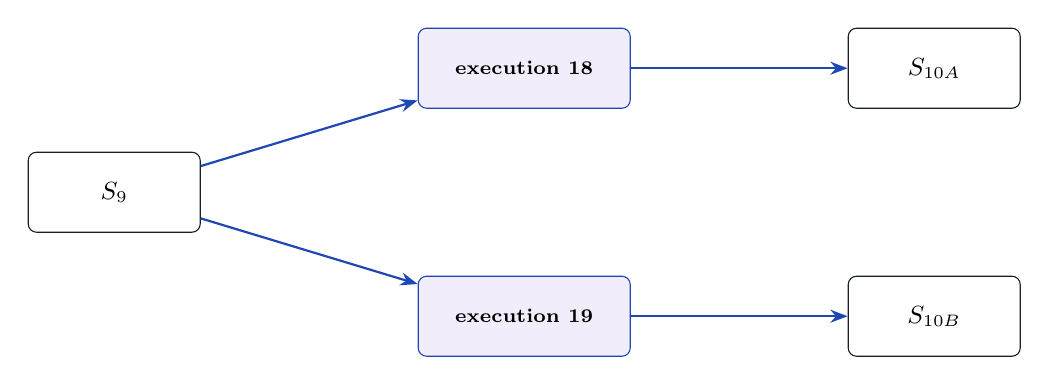
\begin{tikzpicture}[
  state/.style={draw=Ink,fill=white,rounded corners=3pt,minimum width=0.86in,minimum height=0.40in,font=\small\bfseries},
  exec/.style={draw=AccentDark,fill=PurplePale,rounded corners=3pt,minimum width=1.06in,minimum height=0.40in,font=\scriptsize\bfseries},
  edge/.style={-{Stealth[length=2.2mm]},thick,draw=AccentDark}
]
  \node[state] (s9) at (0,0) {$S_9$};
  \node[exec] (e18) at (2.05in,0.62in) {execution 18};
  \node[exec] (e19) at (2.05in,-0.62in) {execution 19};
  \node[state] (s10a) at (4.10in,0.62in) {$S_{10A}$};
  \node[state] (s10b) at (4.10in,-0.62in) {$S_{10B}$};
  \draw[edge] (s9) -- (e18);
  \draw[edge] (e18) -- (s10a);
  \draw[edge] (s9) -- (e19);
  \draw[edge] (e19) -- (s10b);
\end{tikzpicture}
\caption{An explicit rerun from the same parent is an intentional fork: each unique Step execution may publish a different sibling successor.}
\label{fig:explicit-step-rerun-fork}
\end{figure}

\subsection{Details intentionally left open}

This direction does not yet select the on-disk serialization or path of
execution records and state manifests, the exact Git checkpoint mechanism, the
projection of artifact occurrences into a Session workspace, the representation
of direct human-produced states, the exact durable automatic-claim key,
crash-and-retry behavior, optional-output publication, merge workspace
materialization, the explicit-rerun interface, or the final generated-prompt
template. Those are implementation choices to refine against the exemplar Playbooks. The
separation among authored definitions, engine-owned runtime materialization,
and immutable state publication is the working architectural commitment.

\clearpage
\section{Worked execution: three-pass serial research loop}

\begin{summarybox}[Variation 2 made concrete]
This section instantiates the serial refinement graph from
Figure~\ref{fig:epistemic-serial-loop}. The example completes three passes
through Frame, Discover, Appraise, and Design. The first two Design executions
publish a new \artifact{research-agenda.md} occurrence, which makes Frame
applicable again. The third publishes \artifact{research-complete.md} but no new
agenda occurrence. The absence of a new agenda leaves Frame ineligible, so the
Playbook becomes quiescent. The completion marker documents the agent's
decision; it is not an engine stop signal. The three pass labels are
explanatory only: the engine stores no loop object, loop identifier, iteration
counter, or backward state edge.
\end{summarybox}

The example uses a single primary handoff per ordinary Step. The initial state
contains a seed \artifact{research-agenda.md}. A continuing Design execution
replaces that logical file with a newly published occurrence in its successor
state. A final Design execution leaves the last agenda occurrence inherited
but does not republish it.

\subsection{Four representations instantiated by the serial loop}

\begin{longtable}{@{}L{1.34in}L{0.82in}L{4.38in}@{}}
\toprule
\textbf{Representation} & \textbf{Owner} & \textbf{Concrete form in this example} \\
\midrule
\endfirsthead
\toprule
\textbf{Representation} & \textbf{Owner} & \textbf{Concrete form in this example} \\
\midrule
\endhead
Playbook source & Author & Four reusable Step definitions and their Markdown instructions in one file. No pass number, state identifier, execution identifier, or Git checkpoint appears in the source. \\
Step execution records & Engine & Twelve records, \texttt{exec-01} through \texttt{exec-12}, each binding one Step revision to one exact primary artifact occurrence and one parent state. \\
Sealed state manifests & Engine & Thirteen full states, \texttt{state-0} through \texttt{state-12}. Every successful execution publishes one successor with an explicit parent, checkpoint, full current artifact map, and creating provenance. \\
Generated Session contexts & Engine & Twelve runtime preambles containing the exact execution, state, checkpoint, workspace, primary handoff occurrence, predecessor, output contract, and completion operation for that Session. \\
\bottomrule
\end{longtable}

\subsection{Author-written Playbook source}

The following is the complete literal source used by this worked trace. The
\texttt{sketch-0} label is deliberate. The \texttt{inputs},
\texttt{required}, \texttt{possible}, and authored \artifact{NewFor} spellings
make this example executable on paper without claiming that the final file
schema has been selected.

\lstinputlisting[
  style=playbook,
  basicstyle=\ttfamily\tiny,
  numbers=left,
  numberstyle=\tiny\color{Muted},
  numbersep=7pt,
  stepnumber=1,
  numberblanklines=false,
  xleftmargin=2.1em,
  framexleftmargin=1.6em,
  captionpos=b,
  caption={Complete serial research-refinement Playbook specimen.},
  label={lst:serial-research-loop-playbook}
]{docs/architecture/playbook-execution-model/v1/playbook-examples/02-serial-research-loop.md}

\subsection{Engine-owned execution and state records}

\subsubsection{Identifier legend}

\begin{lstlisting}[style=playbook]
states      = state-0 ... state-12
executions  = exec-01 ... exec-12
sessions    = session-01 ... session-12
checkpoints = checkpoint-000 ... checkpoint-012
\end{lstlisting}

All twelve executions use Step-definition revision 1, start automatically, use
one Session, complete successfully, and publish exactly one successor. This
one-Session choice follows the authoring recommendation; the runtime still
permits continuation Sessions inside any one atomic execution.

\subsubsection{One record pair expanded}

The fourth execution and its successor illustrate the complete pairing. The
agent writes normal filenames and calls \texttt{step\_complete}; the engine
creates every identifier and provenance field shown here.

\begin{lstlisting}[style=playbook]
StepExecution exec-04
  step_definition   = develop-design@1
  parent_states     = [state-3]
  input_checkpoint  = checkpoint-003
  input_binding     = [evidence-synthesis.md@exec-03]
  sessions          = [session-04]
  started_by        = automatic
  lifecycle         = completed
  started_at        = 2026-08-29T12:03:00Z
  accepted_at       = 2026-08-29T12:04:00Z
  outcome           = success
  result_state      = state-4
  published         = [design.md@exec-04,
                       research-agenda.md@exec-04]

StateManifest state-4
  parents           = [state-3]
  git_checkpoint    = checkpoint-004
  artifacts         = [research-agenda.md@exec-04,
                       research-questions.md@exec-01,
                       source-map.md@exec-02,
                       evidence-synthesis.md@exec-03,
                       design.md@exec-04]
  created_by        = exec-04
  session_ids       = [session-04]
  input_binding     = [evidence-synthesis.md@exec-03]
  output_contract   = {required: [design.md],
                       possible: [research-agenda.md,
                                  research-complete.md]}
  published_outputs = [design.md@exec-04,
                       research-agenda.md@exec-04]
  accepted_at       = 2026-08-29T12:04:00Z
\end{lstlisting}

\subsubsection{All twelve Step execution records}

Each row below is one complete successful transition. The occurrence suffix is
engine provenance, not part of the physical filename seen by the agent.

The compact occurrence notation used in both ledgers is:

\begin{lstlisting}[style=playbook]
G = research-agenda.md       Q = research-questions.md
M = source-map.md            E = evidence-synthesis.md
D = design.md                C = research-complete.md
\end{lstlisting}

{\scriptsize
\begin{longtable}{@{}L{0.30in}L{0.82in}L{1.42in}L{0.84in}L{2.32in}@{}}
\toprule
\textbf{Pass} & \textbf{Execution / Session} & \textbf{Step and states} & \textbf{Exact input binding} & \textbf{Newly published occurrences} \\
\midrule
\endfirsthead
\toprule
\textbf{Pass} & \textbf{Execution / Session} & \textbf{Step and states} & \textbf{Exact input binding} & \textbf{Newly published occurrences} \\
\midrule
\endhead
1 & \texttt{exec-01} / \texttt{session-01} & Frame; \texttt{state-0} \(\to\) \texttt{state-1} & \(G@\mathrm{seed\mbox{-}01}\) & \(Q@01\) \\
1 & \texttt{exec-02} / \texttt{session-02} & Discover; \texttt{state-1} \(\to\) \texttt{state-2} & \(Q@01\) & \(M@02\) \\
1 & \texttt{exec-03} / \texttt{session-03} & Appraise; \texttt{state-2} \(\to\) \texttt{state-3} & \(M@02\) & \(E@03\) \\
1 & \texttt{exec-04} / \texttt{session-04} & Design; \texttt{state-3} \(\to\) \texttt{state-4} & \(E@03\) & \(D@04, G@04\) \\
2 & \texttt{exec-05} / \texttt{session-05} & Frame; \texttt{state-4} \(\to\) \texttt{state-5} & \(G@04\) & \(Q@05\) \\
2 & \texttt{exec-06} / \texttt{session-06} & Discover; \texttt{state-5} \(\to\) \texttt{state-6} & \(Q@05\) & \(M@06\) \\
2 & \texttt{exec-07} / \texttt{session-07} & Appraise; \texttt{state-6} \(\to\) \texttt{state-7} & \(M@06\) & \(E@07\) \\
2 & \texttt{exec-08} / \texttt{session-08} & Design; \texttt{state-7} \(\to\) \texttt{state-8} & \(E@07\) & \(D@08, G@08\) \\
3 & \texttt{exec-09} / \texttt{session-09} & Frame; \texttt{state-8} \(\to\) \texttt{state-9} & \(G@08\) & \(Q@09\) \\
3 & \texttt{exec-10} / \texttt{session-10} & Discover; \texttt{state-9} \(\to\) \texttt{state-10} & \(Q@09\) & \(M@10\) \\
3 & \texttt{exec-11} / \texttt{session-11} & Appraise; \texttt{state-10} \(\to\) \texttt{state-11} & \(M@10\) & \(E@11\) \\
3 & \texttt{exec-12} / \texttt{session-12} & Design; \texttt{state-11} \(\to\) \texttt{state-12} & \(E@11\) & \(D@12, C@12\) \\
\bottomrule
\end{longtable}
}

\subsubsection{Every successor is a full state}

Using the same legend, an occurrence such as \(G@04\) means
\texttt{research-agenda.md@exec-04}. The table is the full current artifact map
for every state, not an output delta. It abbreviates
\texttt{checkpoint-000} through \texttt{checkpoint-012} as
\texttt{000} through \texttt{012}.

{\scriptsize
\begin{longtable}{@{}L{0.62in}L{0.76in}L{0.90in}L{3.65in}@{}}
\toprule
\textbf{State} & \textbf{Parent} & \textbf{Checkpoint / creator} & \textbf{Full current artifact map} \\
\midrule
\endfirsthead
\toprule
\textbf{State} & \textbf{Parent} & \textbf{Checkpoint / creator} & \textbf{Full current artifact map} \\
\midrule
\endhead
\texttt{state-0} & none & \texttt{000} / seed & \(G@\mathrm{seed\mbox{-}01}\) \\
\texttt{state-1} & \texttt{state-0} & \texttt{001} / \texttt{exec-01} & \(G@\mathrm{seed\mbox{-}01}, Q@01\) \\
\texttt{state-2} & \texttt{state-1} & \texttt{002} / \texttt{exec-02} & \(G@\mathrm{seed\mbox{-}01}, Q@01, M@02\) \\
\texttt{state-3} & \texttt{state-2} & \texttt{003} / \texttt{exec-03} & \(G@\mathrm{seed\mbox{-}01}, Q@01, M@02, E@03\) \\
\texttt{state-4} & \texttt{state-3} & \texttt{004} / \texttt{exec-04} & \(G@04, Q@01, M@02, E@03, D@04\) \\
\texttt{state-5} & \texttt{state-4} & \texttt{005} / \texttt{exec-05} & \(G@04, Q@05, M@02, E@03, D@04\) \\
\texttt{state-6} & \texttt{state-5} & \texttt{006} / \texttt{exec-06} & \(G@04, Q@05, M@06, E@03, D@04\) \\
\texttt{state-7} & \texttt{state-6} & \texttt{007} / \texttt{exec-07} & \(G@04, Q@05, M@06, E@07, D@04\) \\
\texttt{state-8} & \texttt{state-7} & \texttt{008} / \texttt{exec-08} & \(G@08, Q@05, M@06, E@07, D@08\) \\
\texttt{state-9} & \texttt{state-8} & \texttt{009} / \texttt{exec-09} & \(G@08, Q@09, M@06, E@07, D@08\) \\
\texttt{state-10} & \texttt{state-9} & \texttt{010} / \texttt{exec-10} & \(G@08, Q@09, M@10, E@07, D@08\) \\
\texttt{state-11} & \texttt{state-10} & \texttt{011} / \texttt{exec-11} & \(G@08, Q@09, M@10, E@11, D@08\) \\
\texttt{state-12} & \texttt{state-11} & \texttt{012} / \texttt{exec-12} & \(G@08, Q@09, M@10, E@11, D@12, C@12\) \\
\bottomrule
\end{longtable}
}

\subsection{Engine-generated Session context}

For this trace, the illustrative runtime root is
\texttt{/runtime/serial-research}. The path is exact within the example but
does not select a production directory layout. Each packet below is the
engine-generated preamble for one Session; the engine appends the matching
authored instruction section from Listing~\ref{lst:serial-research-loop-playbook}.
The primary input uses a normal filename, while
\texttt{resolved\_occurrence} exposes the immutable provenance that selected
that file version.  Each preamble states only the completion contract known at
launch.  The accepted completion calls shown after each pass are later outcome
records, not part of the Session context.

\subsubsection{Pass 1 contexts}

\begin{lstlisting}[style=playbook,basicstyle=\ttfamily\tiny]
[exec-01 / session-01]
step=Frame / Refine Questions (frame-questions@1)
input_state=state-0
input_checkpoint=checkpoint-000
workspace=/runtime/serial-research/exec-01/workspace
artifacts=/runtime/serial-research/exec-01/workspace/artifacts
primary_input=research-agenda.md
resolved_occurrence=research-agenda.md@seed-01
predecessor=human seed seed-01
required_outputs=[research-questions.md]
completion_contract=step_complete(publish=["research-questions.md"])

[exec-02 / session-02]
step=Discover Sources (discover-sources@1)
input_state=state-1
input_checkpoint=checkpoint-001
workspace=/runtime/serial-research/exec-02/workspace
artifacts=/runtime/serial-research/exec-02/workspace/artifacts
primary_input=research-questions.md
resolved_occurrence=research-questions.md@exec-01
predecessor=Frame / Refine Questions, exec-01
required_outputs=[source-map.md]
completion_contract=step_complete(publish=["source-map.md"])

[exec-03 / session-03]
step=Appraise + Synthesize Evidence (appraise-and-synthesize@1)
input_state=state-2
input_checkpoint=checkpoint-002
workspace=/runtime/serial-research/exec-03/workspace
artifacts=/runtime/serial-research/exec-03/workspace/artifacts
primary_input=source-map.md
resolved_occurrence=source-map.md@exec-02
predecessor=Discover Sources, exec-02
required_outputs=[evidence-synthesis.md]
completion_contract=step_complete(publish=["evidence-synthesis.md"])

[exec-04 / session-04]
step=Develop / Revise Design (develop-design@1)
input_state=state-3
input_checkpoint=checkpoint-003
workspace=/runtime/serial-research/exec-04/workspace
artifacts=/runtime/serial-research/exec-04/workspace/artifacts
primary_input=evidence-synthesis.md
resolved_occurrence=evidence-synthesis.md@exec-03
predecessor=Appraise + Synthesize Evidence, exec-03
required_outputs=[design.md]
possible_outputs=[research-agenda.md,research-complete.md]
instruction=publish exactly one decision handoff
completion_contract=publish design.md plus exactly one possible output
\end{lstlisting}

\noindent\textbf{Accepted outcomes after pass 1 (not Session context).}
\begin{lstlisting}[style=playbook,basicstyle=\ttfamily\scriptsize]
exec-01 accepted step_complete(publish=["research-questions.md"])
exec-02 accepted step_complete(publish=["source-map.md"])
exec-03 accepted step_complete(publish=["evidence-synthesis.md"])
exec-04 accepted step_complete(publish=["design.md","research-agenda.md"])
\end{lstlisting}

\subsubsection{Pass 2 contexts}

\begin{lstlisting}[style=playbook,basicstyle=\ttfamily\tiny]
[exec-05 / session-05]
step=Frame / Refine Questions (frame-questions@1)
input_state=state-4
input_checkpoint=checkpoint-004
workspace=/runtime/serial-research/exec-05/workspace
artifacts=/runtime/serial-research/exec-05/workspace/artifacts
primary_input=research-agenda.md
resolved_occurrence=research-agenda.md@exec-04
predecessor=Develop / Revise Design, exec-04
required_outputs=[research-questions.md]
completion_contract=step_complete(publish=["research-questions.md"])

[exec-06 / session-06]
step=Discover Sources (discover-sources@1)
input_state=state-5
input_checkpoint=checkpoint-005
workspace=/runtime/serial-research/exec-06/workspace
artifacts=/runtime/serial-research/exec-06/workspace/artifacts
primary_input=research-questions.md
resolved_occurrence=research-questions.md@exec-05
predecessor=Frame / Refine Questions, exec-05
required_outputs=[source-map.md]
completion_contract=step_complete(publish=["source-map.md"])

[exec-07 / session-07]
step=Appraise + Synthesize Evidence (appraise-and-synthesize@1)
input_state=state-6
input_checkpoint=checkpoint-006
workspace=/runtime/serial-research/exec-07/workspace
artifacts=/runtime/serial-research/exec-07/workspace/artifacts
primary_input=source-map.md
resolved_occurrence=source-map.md@exec-06
predecessor=Discover Sources, exec-06
required_outputs=[evidence-synthesis.md]
completion_contract=step_complete(publish=["evidence-synthesis.md"])

[exec-08 / session-08]
step=Develop / Revise Design (develop-design@1)
input_state=state-7
input_checkpoint=checkpoint-007
workspace=/runtime/serial-research/exec-08/workspace
artifacts=/runtime/serial-research/exec-08/workspace/artifacts
primary_input=evidence-synthesis.md
resolved_occurrence=evidence-synthesis.md@exec-07
predecessor=Appraise + Synthesize Evidence, exec-07
required_outputs=[design.md]
possible_outputs=[research-agenda.md,research-complete.md]
instruction=publish exactly one decision handoff
completion_contract=publish design.md plus exactly one possible output
\end{lstlisting}

\noindent\textbf{Accepted outcomes after pass 2 (not Session context).}
\begin{lstlisting}[style=playbook,basicstyle=\ttfamily\scriptsize]
exec-05 accepted step_complete(publish=["research-questions.md"])
exec-06 accepted step_complete(publish=["source-map.md"])
exec-07 accepted step_complete(publish=["evidence-synthesis.md"])
exec-08 accepted step_complete(publish=["design.md","research-agenda.md"])
\end{lstlisting}

\subsubsection{Pass 3 contexts}

\begin{lstlisting}[style=playbook,basicstyle=\ttfamily\tiny]
[exec-09 / session-09]
step=Frame / Refine Questions (frame-questions@1)
input_state=state-8
input_checkpoint=checkpoint-008
workspace=/runtime/serial-research/exec-09/workspace
artifacts=/runtime/serial-research/exec-09/workspace/artifacts
primary_input=research-agenda.md
resolved_occurrence=research-agenda.md@exec-08
predecessor=Develop / Revise Design, exec-08
required_outputs=[research-questions.md]
completion_contract=step_complete(publish=["research-questions.md"])

[exec-10 / session-10]
step=Discover Sources (discover-sources@1)
input_state=state-9
input_checkpoint=checkpoint-009
workspace=/runtime/serial-research/exec-10/workspace
artifacts=/runtime/serial-research/exec-10/workspace/artifacts
primary_input=research-questions.md
resolved_occurrence=research-questions.md@exec-09
predecessor=Frame / Refine Questions, exec-09
required_outputs=[source-map.md]
completion_contract=step_complete(publish=["source-map.md"])

[exec-11 / session-11]
step=Appraise + Synthesize Evidence (appraise-and-synthesize@1)
input_state=state-10
input_checkpoint=checkpoint-010
workspace=/runtime/serial-research/exec-11/workspace
artifacts=/runtime/serial-research/exec-11/workspace/artifacts
primary_input=source-map.md
resolved_occurrence=source-map.md@exec-10
predecessor=Discover Sources, exec-10
required_outputs=[evidence-synthesis.md]
completion_contract=step_complete(publish=["evidence-synthesis.md"])

[exec-12 / session-12]
step=Develop / Revise Design (develop-design@1)
input_state=state-11
input_checkpoint=checkpoint-011
workspace=/runtime/serial-research/exec-12/workspace
artifacts=/runtime/serial-research/exec-12/workspace/artifacts
primary_input=evidence-synthesis.md
resolved_occurrence=evidence-synthesis.md@exec-11
predecessor=Appraise + Synthesize Evidence, exec-11
required_outputs=[design.md]
possible_outputs=[research-agenda.md,research-complete.md]
instruction=publish exactly one decision handoff
completion_contract=publish design.md plus exactly one possible output
\end{lstlisting}

\noindent\textbf{Accepted outcomes after pass 3 (not Session context).}
\begin{lstlisting}[style=playbook,basicstyle=\ttfamily\scriptsize]
exec-09 accepted step_complete(publish=["research-questions.md"])
exec-10 accepted step_complete(publish=["source-map.md"])
exec-11 accepted step_complete(publish=["evidence-synthesis.md"])
exec-12 accepted step_complete(publish=["design.md","research-complete.md"])
\end{lstlisting}

These are twelve different execution contexts even though the Playbook has
only four Step definitions. In particular, \texttt{exec-01},
\texttt{exec-05}, and \texttt{exec-09} all use the same Frame definition but
receive different parent states and different exact
\artifact{research-agenda.md} occurrences.

\subsection{State to execution to state}

\subsubsection{Concrete forward-only lineage}

The logical graph contains a back-edge, but the concrete history is this
ordinary acyclic chain:

\begin{lstlisting}[style=playbook]
Pass 1
state-0 --exec-01 Frame-----> state-1
state-1 --exec-02 Discover--> state-2
state-2 --exec-03 Appraise--> state-3
state-3 --exec-04 Design----> state-4

Pass 2
state-4 --exec-05 Frame-----> state-5
state-5 --exec-06 Discover--> state-6
state-6 --exec-07 Appraise--> state-7
state-7 --exec-08 Design----> state-8

Pass 3
state-8 --exec-09 Frame-----> state-9
state-9 --exec-10 Discover--> state-10
state-10 --exec-11 Appraise--> state-11
state-11 --exec-12 Design----> state-12
\end{lstlisting}

The displayed pass boundaries do not exist in runtime state. They merely group
twelve forward transitions so a human can see three applications of the same
four-definition process.

\subsubsection{Literal handoff contents for the three passes}

The following intentionally compact files are the complete handoff payloads for
this worked trace. They demonstrate occurrence and control semantics rather
than claiming to be an adequate literature review.

\medskip
\noindent\textbf{Seed and pass 1.}\par\smallskip

\begin{lstlisting}[style=playbook,basicstyle=\ttfamily\scriptsize]
[research-agenda.md@seed-01]
Determine how a state-based Playbook can repeat research work
without introducing a first-class loop construct.

[research-questions.md@exec-01]
Q1. What runtime identity distinguishes new work from a
    persistent artifact that has already been handled?
Q2. How can Design request another research pass without
    requiring the engine to interpret prose?

[source-map.md@exec-02]
Q1 <- planning operators and grounded-action identity
Q1 <- event provenance and idempotent consumption
Q2 <- named completion and decision artifacts

[evidence-synthesis.md@exec-03]
Q1: partially answered. Exact artifact occurrences are a
    promising unit of work, but consumer provenance is open.
Q2: partially answered. A named marker can request another
    pass, but publication semantics need definition.

[design.md@exec-04]
Draft 1: identify every published artifact occurrence by
logical name and producing execution.

[research-agenda.md@exec-04]
R1. Define when an occurrence is new for one Step definition.
R2. Distinguish duplicate suppression from explicit reruns.
\end{lstlisting}

\medskip
\noindent\textbf{Pass 2.}\par\smallskip

\begin{lstlisting}[style=playbook,basicstyle=\ttfamily\scriptsize]
[research-questions.md@exec-05]
Q3. What provenance makes NewFor consumer-specific?
Q4. How can Design publish a continuation or completion marker
    without inherited files being mistaken for new outputs?

[source-map.md@exec-06]
Q3 <- event-consumer offsets and idempotency-key mechanisms
Q4 <- transaction validation and finite outcome contracts

[evidence-synthesis.md@exec-07]
Q3: answered for this design pass. Successful provenance can
    record consumption of one exact input occurrence.
Q4: partially answered. Validation must concern occurrences
    published now, not inherited file existence.

[design.md@exec-08]
Draft 2: derive NewFor from immutable successful-execution
provenance and keep explicit human reruns distinct.

[research-agenda.md@exec-08]
R3. Define the publication boundary between inherited files
    and outputs of the current execution.
R4. Confirm how the final pass becomes quiescent.
\end{lstlisting}

\medskip
\noindent\textbf{Pass 3.}\par\smallskip

\begin{lstlisting}[style=playbook,basicstyle=\ttfamily\scriptsize]
[research-questions.md@exec-09]
Q5. How does explicit publication distinguish an old agenda
    from a newly emitted agenda occurrence?
Q6. In what order do validation, checkpointing, manifest
    writing, and state visibility occur?

[source-map.md@exec-10]
Q5 <- explicit output-set and immutable provenance mechanisms
Q6 <- transactional publication and immutable-log mechanisms

[evidence-synthesis.md@exec-11]
Q5: answered for this trace. Only names in the accepted
    publication set receive new occurrences.
Q6: answered. Validate and checkpoint before atomically
    exposing the successor manifest to evaluation.

[design.md@exec-12]
Draft 3: complete occurrence-specific consumption and atomic
state publication, with no loop object or mutable cursor.

[research-complete.md@exec-12]
No material research question remains open for this scope.
Retained implementation details are documented separately.
\end{lstlisting}

\subsubsection{Eligibility after every publication}

Every newly sealed state wakes evaluation of all four definitions. In this
trace, exactly one new binding is eligible until the final state:

{\scriptsize
\begin{longtable}{@{}L{0.72in}L{1.35in}L{4.00in}@{}}
\toprule
\textbf{State} & \textbf{Newly eligible work} & \textbf{Exact reason} \\
\midrule
\endfirsthead
\toprule
\textbf{State} & \textbf{Newly eligible work} & \textbf{Exact reason} \\
\midrule
\endhead
\texttt{state-0} & Frame \texttt{exec-01} & \(G@\mathrm{seed\mbox{-}01}\) is a valid Frame binding and has not been successfully consumed by Frame. \\
\texttt{state-1} & Discover \texttt{exec-02} & \(Q@01\) is new for Discover; Frame has consumed the seed agenda occurrence. \\
\texttt{state-2} & Appraise \texttt{exec-03} & \(M@02\) is new for Appraise; earlier bindings are consumed. \\
\texttt{state-3} & Design \texttt{exec-04} & \(E@03\) is new for Design. \\
\texttt{state-4} & Frame \texttt{exec-05} & Design published \(G@04\), a new Frame binding distinct from the consumed seed occurrence. \\
\texttt{state-5} & Discover \texttt{exec-06} & \(Q@05\) is new for Discover; \(G@04\) is now consumed by Frame. \\
\texttt{state-6} & Appraise \texttt{exec-07} & \(M@06\) is new for Appraise. \\
\texttt{state-7} & Design \texttt{exec-08} & \(E@07\) is new for Design. \\
\texttt{state-8} & Frame \texttt{exec-09} & Design published \(G@08\), a new Frame binding distinct from \(G@04\). \\
\texttt{state-9} & Discover \texttt{exec-10} & \(Q@09\) is new for Discover; \(G@08\) is now consumed by Frame. \\
\texttt{state-10} & Appraise \texttt{exec-11} & \(M@10\) is new for Appraise. \\
\texttt{state-11} & Design \texttt{exec-12} & \(E@11\) is new for Design. \\
\texttt{state-12} & none; quiescent & Design published \(C@12\), not a new agenda. The current \(G@08\) occurrence was already consumed by Frame in \texttt{exec-09}; every other current primary binding was likewise consumed by its downstream Step. \\
\bottomrule
\end{longtable}
}

\begin{decisionbox}{TealPale}
\textbf{Requirement exposed by the loop.} State sealing must distinguish files
inherited from the parent from artifacts intentionally published by the current
execution. Otherwise the final Design workspace still contains
\artifact{research-agenda.md}, and the engine could incorrectly assign it a new
occurrence and start a fourth pass. An explicit
\texttt{step\_complete(publish = [...])} set is one simple representation of
the requirement; the exact API remains open.
\end{decisionbox}

\subsubsection{Why the third pass stops}

\texttt{state-12} still contains \texttt{research-agenda.md@exec-08} as its
current agenda file because states are complete snapshots and the final Design
execution did not delete it. That occurrence is not stale and is not globally
consumed. The precise fact is narrower: Frame revision 1 successfully consumed
that exact binding in \texttt{exec-09}. Since \texttt{exec-12} did not publish
a new agenda occurrence, \artifact{NewFor} is false for Frame and no fourth
automatic execution is created.

All earlier automatic activations exposed by \texttt{state-0} through
\texttt{state-11} have already been claimed and completed in this trace. Their
durable execution and successful-consumption records prevent reevaluation of
those preserved states from silently launching duplicates. The exact durable
claim key remains open, as Section~23 records; the quiescence statement here is
scoped to the twelve automatic activations enumerated above.

The Playbook is quiescent rather than permanently terminated. A later human or
agentic execution may publish another \artifact{research-agenda.md} occurrence
from any selected state, after which ordinary evaluation may make Frame
applicable again on that branch.

\subsection{Details intentionally left open}

This worked trace deliberately chooses one provisional surface so every value
can be written down. It does not settle whether \artifact{NewFor} appears in
authored syntax or is an implicit once-per-binding activation rule; whether
\texttt{inputs} is the authoritative binding declaration; how possible outputs
are serialized; the provenance scope used across sibling branches; failure,
retry, claim, and crash recovery; or the physical checkpoint, manifest, and
runtime-path layout.

Marker exclusivity remains an agent-instruction responsibility in V1. The
engine records the exact output set submitted at accepted completion, but it
does not semantically decide whether the agent should have continued or
finished. The durable requirement is only that inherited
\artifact{research-agenda.md} is not silently republished when the final
execution publishes \artifact{research-complete.md}.

\clearpage
\section{Worked execution: three-pass parallel appraisal and merge}

\begin{summarybox}[Variation 3 made concrete]
This section instantiates the parallel-appraisal graph from
Figure~\ref{fig:epistemic-parallel-appraisal}. Three research passes discover
four, three, and five question--source pairs respectively. The same five Step
definitions materialize as 27 executions and 28 immutable states. Each
Discover execution freezes one explicit finite expansion; Appraise executions
fan out into isolated sibling states; question Synthesis executions combine
exact group results; and Design combines the question syntheses. The concrete
history is a forward-only DAG even though the reusable dependency graph also
permits another outer pass.
\end{summarybox}

The varying cardinalities are intentional. Pass 1 uses the four pairs drawn in
Figure~\ref{fig:epistemic-parallel-appraisal}. Pass 2 discovers three pairs,
including one question with only one useful source. Pass 3 discovers five
pairs, including one three-source question. The Playbook source contains none
of these counts, pair identifiers, pass labels, runtime state identifiers, or
execution identifiers.

\subsection{Four representations instantiated by parallel appraisal}

\begin{longtable}{@{}L{1.34in}L{0.82in}L{4.38in}@{}}
\toprule
\textbf{Representation} & \textbf{Owner} & \textbf{Concrete form in this example} \\
\midrule
\endfirsthead
\toprule
\textbf{Representation} & \textbf{Owner} & \textbf{Concrete form in this example} \\
\midrule
\endhead
Playbook source & Author & Five reusable definitions and their Markdown instructions. Collection, grounding, readiness, and merge declarations contain no concrete expansion members. \\
Step execution records & Engine & Twenty-seven records, \texttt{exec-01} through \texttt{exec-27}. Twelve use the one Appraise definition, six use the one question-Synthesis definition, and three use the one Design definition. \\
Sealed state manifests & Engine & Twenty-eight full states, \texttt{state-0} through \texttt{state-27}, with ordinary, sibling, one-parent Synthesis, multi-parent Synthesis, and multi-parent Design lineage. \\
Generated Session contexts & Engine & Twenty-seven preambles containing the exact ordinary input state or merge-request source, its checkpoint, workspace, grounded collection member or group, authorized candidate states and checkpoints, output paths, and prospective completion contracts. Accepted completion outcomes are recorded afterward. \\
\bottomrule
\end{longtable}

\subsection{Author-written Playbook source}

The following is the complete literal source used by this trace. Its
\texttt{sketch-0} collection surface is deliberately provisional. The source
defines fixed reusable work; Discover supplies finite runtime members through
accepted completion.

\lstinputlisting[
  style=playbook,
  basicstyle=\ttfamily\tiny,
  numbers=left,
  numberstyle=\tiny\color{Muted},
  numbersep=7pt,
  stepnumber=1,
  numberblanklines=false,
  xleftmargin=2.1em,
  framexleftmargin=1.6em,
  captionpos=b,
  caption={Complete parallel research-appraisal Playbook specimen.},
  label={lst:parallel-appraisal-playbook}
]{docs/architecture/playbook-execution-model/v1/playbook-examples/03-parallel-appraisal.md}

\subsection{Engine-owned execution and state records}

\subsubsection{Identifier and artifact legend}

\begin{lstlisting}[style=playbook]
states       = state-0 ... state-27
executions   = exec-01  ... exec-27
sessions     = session-01 ... session-27
checkpoints  = checkpoint-000 ... checkpoint-027

G   = research-agenda.md       Q   = research-questions.md
M   = source-map.md            Z   = design-request.md
Pxy = appraisal-request-Qx-Y.md
Axy = appraisal-result-Qx-Y.md
Tx  = question-synthesis-request-Qx.md
Yx  = question-synthesis-Qx.md
D   = design.md                C   = research-complete.md
\end{lstlisting}

An occurrence suffix identifies the publishing execution. For example,
\texttt{P1A@02} is the Q1/A appraisal-request occurrence published by
\texttt{exec-02}. The suffix is manifest provenance, not part of the filename
seen by an agent. The engine also writes one immutable expansion record for
each Discover success:

\begin{lstlisting}[style=playbook,basicstyle=\ttfamily\scriptsize]
K02 = expansion@exec-02
  appraisal groups: Q1=[P1A@02,P1B@02]
                    Q2=[P2B@02,P2C@02]
  synthesis requests: [T1@02,T2@02]
  design request: Z@02 requires [Q1,Q2]

K11 = expansion@exec-11
  appraisal groups: Q3=[P3D@11,P3E@11]
                    Q4=[P4F@11]
  synthesis requests: [T3@11,T4@11]
  design request: Z@11 requires [Q3,Q4]

K19 = expansion@exec-19
  appraisal groups: Q5=[P5G@19,P5H@19,P5I@19]
                    Q6=[P6H@19,P6J@19]
  synthesis requests: [T5@19,T6@19]
  design request: Z@19 requires [Q5,Q6]
\end{lstlisting}

These memberships are authoritative structured provenance. No glob, regular
expression, filename prefix, or Markdown parser reconstructs them. The
collection identity includes its producing Discover execution, so reusing a
question or source key in another pass cannot accidentally reuse an older
member.

\subsubsection{Discover success freezes one finite expansion}

The first Discover execution produces one successor state, not four Appraise
states. Its accepted publication contains ordinary files plus an exact
collection declaration:

\begin{lstlisting}[style=playbook,basicstyle=\ttfamily\scriptsize]
StepExecution exec-02
  step_definition   = discover-sources@1
  parent_states     = [state-1]
  input_binding     = [Q@01]
  sessions          = [session-02]
  lifecycle         = completed
  result_state      = state-2
  published         = [M@02,P1A@02,P1B@02,P2B@02,P2C@02,
                       T1@02,T2@02,Z@02]
  frozen_expansion  = K02

StateManifest state-2
  parents           = [state-1]
  produced_by       = exec-02
  git_checkpoint    = checkpoint-002
  artifacts         = full current map shown below
  collection_record = K02
  accepted_at       = 2026-08-29T13:02:00Z
\end{lstlisting}

Only after \texttt{state-2} is visible does the engine ground four independent
executions. Each applies the Appraise definition, receives \texttt{state-2} as
its one parent, and receives one exact request occurrence as its primary
binding.

\subsubsection{One question-Synthesis merge record expanded}

The global V1 readiness barrier for \texttt{K02} reaches four successful
results before either question Synthesis starts. The Q1 execution then receives
only the exact Q1 group as merge input. Candidate exposure is launch context;
selected parents are an accepted-completion outcome:

\begin{lstlisting}[style=playbook,basicstyle=\ttfamily\scriptsize]
StepExecution exec-07
  step_definition      = synthesize-question@1
  grounding            = {expansion: K02, group: Q1}
  readiness_witness    = {K02 appraisal coverage: 4/4}
  authorized_candidates = [
    {state: state-3, result: A1A@03, covers: P1A@02},
    {state: state-4, result: A1B@04, covers: P1B@02}
  ]
  input_binding        = [T1@02,A1A@03,A1B@04]
  sessions             = [session-07]
  lifecycle            = completed
  accepted_selection   = [state-3,state-4]
  result_state         = state-7
  published            = [Y1@07]

StateManifest state-7
  parents              = [state-3,state-4]
  produced_by          = exec-07
  git_checkpoint       = checkpoint-007
  input_binding        = [T1@02,A1A@03,A1B@04]
  published_outputs    = [Y1@07]
  session_ids          = [session-07]
  accepted_at          = 2026-08-29T13:07:00Z
\end{lstlisting}

The engine validates that the declared states are authorized and collectively
cover the entire frozen Q1 group. It does not make the unrelated Q2 Appraise
states parents merely because their success was required by the conservative
global launch barrier.

\subsubsection{The final Design merge record expanded}

The final Design Session is launched with two authorized question-synthesis
candidates but no already-selected parents. The accepted completion supplies
that semantic choice:

\begin{lstlisting}[style=playbook,basicstyle=\ttfamily\scriptsize]
StepExecution exec-27
  step_definition      = develop-design@1
  grounding            = {expansion: K19, design request: Z@19}
  authorized_candidates = [
    {state: state-25, result: Y5@25, covers: K19/Q5},
    {state: state-26, result: Y6@26, covers: K19/Q6}
  ]
  input_binding        = [Z@19,Y5@25,Y6@26]
  sessions             = [session-27]
  lifecycle            = completed
  accepted_selection   = [state-25,state-26]
  result_state         = state-27
  published            = [D@27,C@27]

StateManifest state-27
  parents              = [state-25,state-26]
  produced_by          = exec-27
  git_checkpoint       = checkpoint-027
  input_binding        = [Z@19,Y5@25,Y6@26]
  published_outputs    = [D@27,C@27]
  session_ids          = [session-27]
  accepted_at          = 2026-08-29T13:27:00Z
\end{lstlisting}

The full state still inherits \texttt{G@17}, but \texttt{exec-27} publishes no
new \artifact{research-agenda.md} occurrence. Design's completion therefore
cannot ground a fourth Frame execution.

\subsubsection{All twenty-seven Step execution records}

Every execution below uses Step-definition revision 1, one Session with the
matching number, and one accepted publication. Bracketed sources identify
multi-parent or merge-capable transitions.

{\tiny
\begin{longtable}{@{}L{0.28in}L{0.48in}L{1.42in}L{1.45in}L{2.16in}@{}}
\toprule
\textbf{Pass} & \textbf{Exec} & \textbf{Step; parents to result} & \textbf{Exact binding} & \textbf{Newly published occurrences} \\
\midrule
\endfirsthead
\toprule
\textbf{Pass} & \textbf{Exec} & \textbf{Step; parents to result} & \textbf{Exact binding} & \textbf{Newly published occurrences} \\
\midrule
\endhead
1 & 01 & Frame; 0 to 1 & \texttt{G@seed-01} & \texttt{Q@01} \\
1 & 02 & Discover; 1 to 2 & \texttt{Q@01} & \texttt{M@02, K02: P1A, P1B, P2B, P2C, T1, T2, Z} \\
1 & 03 & Appraise Q1/A; 2 to 3 & \texttt{P1A@02} & \texttt{A1A@03} \\
1 & 04 & Appraise Q1/B; 2 to 4 & \texttt{P1B@02} & \texttt{A1B@04} \\
1 & 05 & Appraise Q2/B; 2 to 5 & \texttt{P2B@02} & \texttt{A2B@05} \\
1 & 06 & Appraise Q2/C; 2 to 6 & \texttt{P2C@02} & \texttt{A2C@06} \\
1 & 07 & Synthesize Q1; [3,4] to 7 & \texttt{T1@02, A1A@03, A1B@04} & \texttt{Y1@07} \\
1 & 08 & Synthesize Q2; [5,6] to 8 & \texttt{T2@02, A2B@05, A2C@06} & \texttt{Y2@08} \\
1 & 09 & Design; [7,8] to 9 & \texttt{Z@02, Y1@07, Y2@08} & \texttt{D@09, G@09} \\
2 & 10 & Frame; 9 to 10 & \texttt{G@09} & \texttt{Q@10} \\
2 & 11 & Discover; 10 to 11 & \texttt{Q@10} & \texttt{M@11, K11: P3D, P3E, P4F, T3, T4, Z} \\
2 & 12 & Appraise Q3/D; 11 to 12 & \texttt{P3D@11} & \texttt{A3D@12} \\
2 & 13 & Appraise Q3/E; 11 to 13 & \texttt{P3E@11} & \texttt{A3E@13} \\
2 & 14 & Appraise Q4/F; 11 to 14 & \texttt{P4F@11} & \texttt{A4F@14} \\
2 & 15 & Synthesize Q3; [12,13] to 15 & \texttt{T3@11, A3D@12, A3E@13} & \texttt{Y3@15} \\
2 & 16 & Synthesize Q4; 14 to 16 & \texttt{T4@11, A4F@14} & \texttt{Y4@16} \\
2 & 17 & Design; [15,16] to 17 & \texttt{Z@11, Y3@15, Y4@16} & \texttt{D@17, G@17} \\
3 & 18 & Frame; 17 to 18 & \texttt{G@17} & \texttt{Q@18} \\
3 & 19 & Discover; 18 to 19 & \texttt{Q@18} & \texttt{M@19, K19: P5G, P5H, P5I, P6H, P6J, T5, T6, Z} \\
3 & 20 & Appraise Q5/G; 19 to 20 & \texttt{P5G@19} & \texttt{A5G@20} \\
3 & 21 & Appraise Q5/H; 19 to 21 & \texttt{P5H@19} & \texttt{A5H@21} \\
3 & 22 & Appraise Q5/I; 19 to 22 & \texttt{P5I@19} & \texttt{A5I@22} \\
3 & 23 & Appraise Q6/H; 19 to 23 & \texttt{P6H@19} & \texttt{A6H@23} \\
3 & 24 & Appraise Q6/J; 19 to 24 & \texttt{P6J@19} & \texttt{A6J@24} \\
3 & 25 & Synthesize Q5; [20,21,22] to 25 & \texttt{T5@19, A5G@20, A5H@21, A5I@22} & \texttt{Y5@25} \\
3 & 26 & Synthesize Q6; [23,24] to 26 & \texttt{T6@19, A6H@23, A6J@24} & \texttt{Y6@26} \\
3 & 27 & Design; [25,26] to 27 & \texttt{Z@19, Y5@25, Y6@26} & \texttt{D@27, C@27} \\
\bottomrule
\end{longtable}
}

\subsubsection{Every successor is a full state}

The following equations specify every current artifact map exactly while
avoiding 28 repetitions of inherited files. In this notation,
\texttt{X + \{occurrences\}} means copy the complete map of \texttt{X}, then
set or replace each named logical path with the listed occurrence.
\texttt{merge(X,Y)} unions the selected parent maps at their common inherited
occurrences; the agent resolves any genuine conflict before publication.

\begin{lstlisting}[style=playbook,basicstyle=\ttfamily\scriptsize]
B02 = {M@02,P1A@02,P1B@02,P2B@02,P2C@02,T1@02,T2@02,Z@02}
B11 = {M@11,P3D@11,P3E@11,P4F@11,T3@11,T4@11,Z@11}
B19 = {M@19,P5G@19,P5H@19,P5I@19,P6H@19,P6J@19,
       T5@19,T6@19,Z@19}

state-0  = {G@seed-01}
state-1  = state-0 + {Q@01}
state-2  = state-1 + B02
state-3  = state-2 + {A1A@03}
state-4  = state-2 + {A1B@04}
state-5  = state-2 + {A2B@05}
state-6  = state-2 + {A2C@06}
state-7  = merge(state-3,state-4) + {Y1@07}
state-8  = merge(state-5,state-6) + {Y2@08}
state-9  = merge(state-7,state-8) + {D@09,G@09}

state-10 = state-9 + {Q@10}
state-11 = state-10 + B11
state-12 = state-11 + {A3D@12}
state-13 = state-11 + {A3E@13}
state-14 = state-11 + {A4F@14}
state-15 = merge(state-12,state-13) + {Y3@15}
state-16 = state-14 + {Y4@16}
state-17 = merge(state-15,state-16) + {D@17,G@17}

state-18 = state-17 + {Q@18}
state-19 = state-18 + B19
state-20 = state-19 + {A5G@20}
state-21 = state-19 + {A5H@21}
state-22 = state-19 + {A5I@22}
state-23 = state-19 + {A6H@23}
state-24 = state-19 + {A6J@24}
state-25 = merge(state-20,state-21,state-22) + {Y5@25}
state-26 = merge(state-23,state-24) + {Y6@26}
state-27 = merge(state-25,state-26) + {D@27,C@27}
\end{lstlisting}

These are full maps, not output deltas. Because \texttt{state-27} does not set
\artifact{research-agenda.md}, its current map still contains \texttt{G@17}.
Likewise, setting a new \artifact{source-map.md}, \artifact{design-request.md},
or \artifact{design.md} path changes the current occurrence without deleting
the earlier occurrence from immutable history.

\subsection{Engine-generated Session context}

For this trace the illustrative runtime root is
\texttt{/runtime/parallel-research}. For every \texttt{exec-NN}, the exact
generated values are:

\begin{lstlisting}[style=playbook]
session    = session-NN
workspace  = /runtime/parallel-research/exec-NN/workspace
artifacts  = /runtime/parallel-research/exec-NN/workspace/artifacts
\end{lstlisting}

The path rule is exact within this example but does not freeze a production
layout. Each compact packet below supplies every varying pre-launch fact. The
engine appends the matching authored instruction section from
Listing~\ref{lst:parallel-appraisal-playbook}. A prospective
\texttt{completion\_contract} never contains the agent's future parent
selection; accepted outcomes are listed separately after each pass.

\subsubsection{Pass 1 contexts}

\begin{lstlisting}[style=playbook,basicstyle=\ttfamily\tiny]
[exec-01 / session-01]
step=Frame / Refine Questions (frame-questions@1)
input=state-0 / checkpoint-000
primary=research-agenda.md; occurrence=G@seed-01
predecessor=human seed seed-01
required=[research-questions.md]
completion_contract=publish [research-questions.md]

[exec-02 / session-02]
step=Discover Sources and Map Plausible Pairs (discover-sources@1)
input=state-1 / checkpoint-001
primary=research-questions.md; occurrence=Q@01
predecessor=Frame exec-01
required=[source-map.md, appraisal-requests,
          question-synthesis-requests, design-request]
completion_contract=publish exact files and finite collection declaration

[exec-03 / session-03]
step=Appraise One Pair (appraise-pair@1)
input=state-2 / checkpoint-002
grounding={expansion:K02,member:Q1/A,group:Q1}
primary=appraisal-request-Q1-A.md; occurrence=P1A@02
required=[appraisal-result-Q1-A.md]
completion_contract=publish [appraisal-result-Q1-A.md]

[exec-04 / session-04]
step=Appraise One Pair (appraise-pair@1)
input=state-2 / checkpoint-002
grounding={expansion:K02,member:Q1/B,group:Q1}
primary=appraisal-request-Q1-B.md; occurrence=P1B@02
required=[appraisal-result-Q1-B.md]
completion_contract=publish [appraisal-result-Q1-B.md]

[exec-05 / session-05]
step=Appraise One Pair (appraise-pair@1)
input=state-2 / checkpoint-002
grounding={expansion:K02,member:Q2/B,group:Q2}
primary=appraisal-request-Q2-B.md; occurrence=P2B@02
required=[appraisal-result-Q2-B.md]
completion_contract=publish [appraisal-result-Q2-B.md]

[exec-06 / session-06]
step=Appraise One Pair (appraise-pair@1)
input=state-2 / checkpoint-002
grounding={expansion:K02,member:Q2/C,group:Q2}
primary=appraisal-request-Q2-C.md; occurrence=P2C@02
required=[appraisal-result-Q2-C.md]
completion_contract=publish [appraisal-result-Q2-C.md]

[exec-07 / session-07]
step=Synthesize One Question (synthesize-question@1)
coverage_gate={expansion:K02,successful:4,required:4}
grounding={group:Q1,primary:T1@02}
request_source=state-2 / checkpoint-002
resolved_binding=[T1@02,A1A@03,A1B@04]
authorized_candidates=[state-3/checkpoint-003/A1A@03,
                       state-4/checkpoint-004/A1B@04]
required=[question-synthesis-Q1.md]
completion_contract=select authorized parents covering Q1; publish required

[exec-08 / session-08]
step=Synthesize One Question (synthesize-question@1)
coverage_gate={expansion:K02,successful:4,required:4}
grounding={group:Q2,primary:T2@02}
request_source=state-2 / checkpoint-002
resolved_binding=[T2@02,A2B@05,A2C@06]
authorized_candidates=[state-5/checkpoint-005/A2B@05,
                       state-6/checkpoint-006/A2C@06]
required=[question-synthesis-Q2.md]
completion_contract=select authorized parents covering Q2; publish required

[exec-09 / session-09]
step=Develop / Revise Design (develop-design@1)
coverage_gate={expansion:K02,question_groups:2/2}
grounding={primary:Z@02}
request_source=state-2 / checkpoint-002
resolved_binding=[Z@02,Y1@07,Y2@08]
authorized_candidates=[state-7/checkpoint-007/Y1@07,
                       state-8/checkpoint-008/Y2@08]
required=[design.md]
possible=[research-agenda.md,research-complete.md]
completion_contract=select complete synthesis parents; publish design plus
                    exactly one decision handoff
\end{lstlisting}

\noindent\textbf{Accepted outcomes after pass 1 (not Session context).}
\begin{lstlisting}[style=playbook,basicstyle=\ttfamily\scriptsize]
exec-01 accepted publish=[Q@01]
exec-02 accepted publish=[M@02,P1A@02,P1B@02,P2B@02,P2C@02,
                          T1@02,T2@02,Z@02]; freeze=K02
exec-03 accepted publish=[A1A@03]
exec-04 accepted publish=[A1B@04]
exec-05 accepted publish=[A2B@05]
exec-06 accepted publish=[A2C@06]
exec-07 accepted parents=[state-3,state-4]; publish=[Y1@07]
exec-08 accepted parents=[state-5,state-6]; publish=[Y2@08]
exec-09 accepted parents=[state-7,state-8]; publish=[D@09,G@09]
\end{lstlisting}

\subsubsection{Pass 2 contexts}

\begin{lstlisting}[style=playbook,basicstyle=\ttfamily\tiny]
[exec-10 / session-10]
step=Frame / Refine Questions (frame-questions@1)
input=state-9 / checkpoint-009
primary=research-agenda.md; occurrence=G@09
predecessor=Design exec-09
required=[research-questions.md]
completion_contract=publish [research-questions.md]

[exec-11 / session-11]
step=Discover Sources and Map Plausible Pairs (discover-sources@1)
input=state-10 / checkpoint-010
primary=research-questions.md; occurrence=Q@10
predecessor=Frame exec-10
required=[source-map.md, appraisal-requests,
          question-synthesis-requests, design-request]
completion_contract=publish exact files and finite collection declaration

[exec-12 / session-12]
step=Appraise One Pair (appraise-pair@1)
input=state-11 / checkpoint-011
grounding={expansion:K11,member:Q3/D,group:Q3}
primary=appraisal-request-Q3-D.md; occurrence=P3D@11
required=[appraisal-result-Q3-D.md]
completion_contract=publish [appraisal-result-Q3-D.md]

[exec-13 / session-13]
step=Appraise One Pair (appraise-pair@1)
input=state-11 / checkpoint-011
grounding={expansion:K11,member:Q3/E,group:Q3}
primary=appraisal-request-Q3-E.md; occurrence=P3E@11
required=[appraisal-result-Q3-E.md]
completion_contract=publish [appraisal-result-Q3-E.md]

[exec-14 / session-14]
step=Appraise One Pair (appraise-pair@1)
input=state-11 / checkpoint-011
grounding={expansion:K11,member:Q4/F,group:Q4}
primary=appraisal-request-Q4-F.md; occurrence=P4F@11
required=[appraisal-result-Q4-F.md]
completion_contract=publish [appraisal-result-Q4-F.md]

[exec-15 / session-15]
step=Synthesize One Question (synthesize-question@1)
coverage_gate={expansion:K11,successful:3,required:3}
grounding={group:Q3,primary:T3@11}
request_source=state-11 / checkpoint-011
resolved_binding=[T3@11,A3D@12,A3E@13]
authorized_candidates=[state-12/checkpoint-012/A3D@12,
                       state-13/checkpoint-013/A3E@13]
required=[question-synthesis-Q3.md]
completion_contract=select authorized parents covering Q3; publish required

[exec-16 / session-16]
step=Synthesize One Question (synthesize-question@1)
coverage_gate={expansion:K11,successful:3,required:3}
grounding={group:Q4,primary:T4@11}
request_source=state-11 / checkpoint-011
resolved_binding=[T4@11,A4F@14]
authorized_candidates=[state-14/checkpoint-014/A4F@14]
required=[question-synthesis-Q4.md]
completion_contract=select the authorized Q4 parent; publish required

[exec-17 / session-17]
step=Develop / Revise Design (develop-design@1)
coverage_gate={expansion:K11,question_groups:2/2}
grounding={primary:Z@11}
request_source=state-11 / checkpoint-011
resolved_binding=[Z@11,Y3@15,Y4@16]
authorized_candidates=[state-15/checkpoint-015/Y3@15,
                       state-16/checkpoint-016/Y4@16]
required=[design.md]
possible=[research-agenda.md,research-complete.md]
completion_contract=select complete synthesis parents; publish design plus
                    exactly one decision handoff
\end{lstlisting}

\newpage
\noindent\textbf{Accepted outcomes after pass 2 (not Session context).}
\begin{lstlisting}[style=playbook,basicstyle=\ttfamily\scriptsize]
exec-10 accepted publish=[Q@10]
exec-11 accepted publish=[M@11,P3D@11,P3E@11,P4F@11,
                          T3@11,T4@11,Z@11]; freeze=K11
exec-12 accepted publish=[A3D@12]
exec-13 accepted publish=[A3E@13]
exec-14 accepted publish=[A4F@14]
exec-15 accepted parents=[state-12,state-13]; publish=[Y3@15]
exec-16 accepted parents=[state-14]; publish=[Y4@16]
exec-17 accepted parents=[state-15,state-16]; publish=[D@17,G@17]
\end{lstlisting}

\subsubsection{Pass 3 contexts}

\begin{lstlisting}[style=playbook,basicstyle=\ttfamily\tiny]
[exec-18 / session-18]
step=Frame / Refine Questions (frame-questions@1)
input=state-17 / checkpoint-017
primary=research-agenda.md; occurrence=G@17
predecessor=Design exec-17
required=[research-questions.md]
completion_contract=publish [research-questions.md]

[exec-19 / session-19]
step=Discover Sources and Map Plausible Pairs (discover-sources@1)
input=state-18 / checkpoint-018
primary=research-questions.md; occurrence=Q@18
predecessor=Frame exec-18
required=[source-map.md, appraisal-requests,
          question-synthesis-requests, design-request]
completion_contract=publish exact files and finite collection declaration

[exec-20 / session-20]
step=Appraise One Pair (appraise-pair@1)
input=state-19 / checkpoint-019
grounding={expansion:K19,member:Q5/G,group:Q5}
primary=appraisal-request-Q5-G.md; occurrence=P5G@19
required=[appraisal-result-Q5-G.md]
completion_contract=publish [appraisal-result-Q5-G.md]

[exec-21 / session-21]
step=Appraise One Pair (appraise-pair@1)
input=state-19 / checkpoint-019
grounding={expansion:K19,member:Q5/H,group:Q5}
primary=appraisal-request-Q5-H.md; occurrence=P5H@19
required=[appraisal-result-Q5-H.md]
completion_contract=publish [appraisal-result-Q5-H.md]

[exec-22 / session-22]
step=Appraise One Pair (appraise-pair@1)
input=state-19 / checkpoint-019
grounding={expansion:K19,member:Q5/I,group:Q5}
primary=appraisal-request-Q5-I.md; occurrence=P5I@19
required=[appraisal-result-Q5-I.md]
completion_contract=publish [appraisal-result-Q5-I.md]

[exec-23 / session-23]
step=Appraise One Pair (appraise-pair@1)
input=state-19 / checkpoint-019
grounding={expansion:K19,member:Q6/H,group:Q6}
primary=appraisal-request-Q6-H.md; occurrence=P6H@19
required=[appraisal-result-Q6-H.md]
completion_contract=publish [appraisal-result-Q6-H.md]

[exec-24 / session-24]
step=Appraise One Pair (appraise-pair@1)
input=state-19 / checkpoint-019
grounding={expansion:K19,member:Q6/J,group:Q6}
primary=appraisal-request-Q6-J.md; occurrence=P6J@19
required=[appraisal-result-Q6-J.md]
completion_contract=publish [appraisal-result-Q6-J.md]

[exec-25 / session-25]
step=Synthesize One Question (synthesize-question@1)
coverage_gate={expansion:K19,successful:5,required:5}
grounding={group:Q5,primary:T5@19}
request_source=state-19 / checkpoint-019
resolved_binding=[T5@19,A5G@20,A5H@21,A5I@22]
authorized_candidates=[state-20/checkpoint-020/A5G@20,
                       state-21/checkpoint-021/A5H@21,
                       state-22/checkpoint-022/A5I@22]
required=[question-synthesis-Q5.md]
completion_contract=select authorized parents covering Q5; publish required

[exec-26 / session-26]
step=Synthesize One Question (synthesize-question@1)
coverage_gate={expansion:K19,successful:5,required:5}
grounding={group:Q6,primary:T6@19}
request_source=state-19 / checkpoint-019
resolved_binding=[T6@19,A6H@23,A6J@24]
authorized_candidates=[state-23/checkpoint-023/A6H@23,
                       state-24/checkpoint-024/A6J@24]
required=[question-synthesis-Q6.md]
completion_contract=select authorized parents covering Q6; publish required

[exec-27 / session-27]
step=Develop / Revise Design (develop-design@1)
coverage_gate={expansion:K19,question_groups:2/2}
grounding={primary:Z@19}
request_source=state-19 / checkpoint-019
resolved_binding=[Z@19,Y5@25,Y6@26]
authorized_candidates=[state-25/checkpoint-025/Y5@25,
                       state-26/checkpoint-026/Y6@26]
required=[design.md]
possible=[research-agenda.md,research-complete.md]
completion_contract=select complete synthesis parents; publish design plus
                    exactly one decision handoff
\end{lstlisting}

\noindent\textbf{Accepted outcomes after pass 3 (not Session context).}
\begin{lstlisting}[style=playbook,basicstyle=\ttfamily\scriptsize]
exec-18 accepted publish=[Q@18]
exec-19 accepted publish=[M@19,P5G@19,P5H@19,P5I@19,P6H@19,P6J@19,
                          T5@19,T6@19,Z@19]; freeze=K19
exec-20 accepted publish=[A5G@20]
exec-21 accepted publish=[A5H@21]
exec-22 accepted publish=[A5I@22]
exec-23 accepted publish=[A6H@23]
exec-24 accepted publish=[A6J@24]
exec-25 accepted parents=[state-20,state-21,state-22]; publish=[Y5@25]
exec-26 accepted parents=[state-23,state-24]; publish=[Y6@26]
exec-27 accepted parents=[state-25,state-26]; publish=[D@27,C@27]
\end{lstlisting}

The 27 contexts use only five definition revisions. In particular, no Appraise
Session is authored in advance for a concrete pair. Discover determines the
finite decomposition, the engine grounds exact instances, and the scheduler
controls how many may run concurrently.

\subsection{State to execution to state}

\subsubsection{Concrete forward-only DAG}

The derived dependency view fans out and later loops, but the concrete history
contains only forward transitions. All Appraises in one pass keep the exact
Discover successor as parent even if siblings finish earlier:

\begin{lstlisting}[style=playbook,basicstyle=\ttfamily\scriptsize]
Pass 1
state-0 -> exec-01 Frame -> state-1 -> exec-02 Discover -> state-2
  state-2 -> exec-03 Appraise Q1/A -> state-3 --+
  state-2 -> exec-04 Appraise Q1/B -> state-4 --+-> exec-07 Synth Q1 -> state-7 --+
  state-2 -> exec-05 Appraise Q2/B -> state-5 --+                                +-> exec-09 Design -> state-9
  state-2 -> exec-06 Appraise Q2/C -> state-6 --+-> exec-08 Synth Q2 -> state-8 --+

Pass 2
state-9 -> exec-10 Frame -> state-10 -> exec-11 Discover -> state-11
  state-11 -> exec-12 Appraise Q3/D -> state-12 --+
  state-11 -> exec-13 Appraise Q3/E -> state-13 --+-> exec-15 Synth Q3 -> state-15 --+
  state-11 -> exec-14 Appraise Q4/F -> state-14 ----> exec-16 Synth Q4 -> state-16 --+-> exec-17 Design -> state-17

Pass 3
state-17 -> exec-18 Frame -> state-18 -> exec-19 Discover -> state-19
  state-19 -> exec-20 Appraise Q5/G -> state-20 --+
  state-19 -> exec-21 Appraise Q5/H -> state-21 --+-> exec-25 Synth Q5 -> state-25 --+
  state-19 -> exec-22 Appraise Q5/I -> state-22 --+                                 +-> exec-27 Design -> state-27
  state-19 -> exec-23 Appraise Q6/H -> state-23 --+                                 |
  state-19 -> exec-24 Appraise Q6/J -> state-24 --+-> exec-26 Synth Q6 -> state-26 --+
\end{lstlisting}

The pass labels are explanatory only. There is no runtime pass object, split
node, join gateway, active branch, or state-history cycle. \texttt{exec-16}
also demonstrates that the same Synthesis definition can publish from one
selected parent when one question has only one appraisal result. ``Merge''
describes the multi-parent runtime case, not a separate authored Step kind.

\subsubsection{Literal handoff contents for all three passes}

The following compact files are the complete handoff payloads for this worked
trace. They demonstrate control, collection, and provenance semantics rather
than claiming to be an adequate literature review.

\medskip
\noindent\textbf{Seed and pass 1: four pair members.}\par\smallskip

\begin{lstlisting}[style=playbook,basicstyle=\ttfamily\scriptsize]
[research-agenda.md@seed-01]
Determine how a state-based Playbook can expand unknown research work,
run it concurrently, and merge it without authored routing nodes.

[research-questions.md@exec-01]
Q1. What immutable identity should ground one dynamically discovered job?
Q2. What provenance is sufficient to combine parallel results safely?

[source-map.md@exec-02]
A = planning operator grounding; B = event provenance and idempotency;
C = multi-parent version history. Retained pairs: Q1/A, Q1/B, Q2/B, Q2/C.

[appraisal-request-Q1-A.md@exec-02]
Evaluate operator grounding as an identity model for Q1. Result: appraisal-result-Q1-A.md.
[appraisal-request-Q1-B.md@exec-02]
Evaluate event provenance as an identity model for Q1. Result: appraisal-result-Q1-B.md.
[appraisal-request-Q2-B.md@exec-02]
Evaluate event provenance for safe combination under Q2. Result: appraisal-result-Q2-B.md.
[appraisal-request-Q2-C.md@exec-02]
Evaluate multi-parent histories for Q2. Result: appraisal-result-Q2-C.md.

[question-synthesis-request-Q1.md@exec-02]
Synthesize Q1 from exact members Q1/A and Q1/B. Result: question-synthesis-Q1.md.
[question-synthesis-request-Q2.md@exec-02]
Synthesize Q2 from exact members Q2/B and Q2/C. Result: question-synthesis-Q2.md.
[design-request.md@exec-02]
Integrate exact syntheses Q1 and Q2 into the state and execution model.

[appraisal-result-Q1-A.md@exec-03]
Grounded operator identity supports one instance per exact bound member.
[appraisal-result-Q1-B.md@exec-04]
Immutable producer, collection, and member keys support replay-safe identity.
[appraisal-result-Q2-B.md@exec-05]
Successful result provenance can witness exact request coverage.
[appraisal-result-Q2-C.md@exec-06]
Explicit selected parents distinguish considered candidates from lineage.

[question-synthesis-Q1.md@exec-07]
Identify work by producing Discover execution, collection, and exact member key.
[question-synthesis-Q2.md@exec-08]
Combine only successful exact result occurrences and record selected parents.

[design.md@exec-09]
Draft 1: freeze explicit collection members, late-ground one Appraise per member,
and require agent-declared parents for question and Design combination.
[research-agenda.md@exec-09]
R1. Test whether cardinality may vary without changing definitions.
R2. Test a question group with only one successful appraisal input.
\end{lstlisting}

\medskip
\noindent\textbf{Pass 2: three pair members.}\par\smallskip

\begin{lstlisting}[style=playbook,basicstyle=\ttfamily\scriptsize]
[research-questions.md@exec-10]
Q3. Can a later Discover execution freeze a different member count safely?
Q4. Does the same Synthesis definition work with one selected parent?

[source-map.md@exec-11]
D = late grounding; E = durable work claims; F = one-source evidence policy.
Retained pairs: Q3/D, Q3/E, Q4/F.

[appraisal-request-Q3-D.md@exec-11]
Evaluate late grounding for Q3. Result: appraisal-result-Q3-D.md.
[appraisal-request-Q3-E.md@exec-11]
Evaluate durable claim identity for Q3. Result: appraisal-result-Q3-E.md.
[appraisal-request-Q4-F.md@exec-11]
Evaluate one-source synthesis semantics for Q4. Result: appraisal-result-Q4-F.md.
[question-synthesis-request-Q3.md@exec-11]
Synthesize Q3 from Q3/D and Q3/E. Result: question-synthesis-Q3.md.
[question-synthesis-request-Q4.md@exec-11]
Synthesize Q4 from Q4/F. Result: question-synthesis-Q4.md.
[design-request.md@exec-11]
Integrate exact syntheses Q3 and Q4 into the current design.

[appraisal-result-Q3-D.md@exec-12]
Definitions remain fixed while explicit collection members ground instances late.
[appraisal-result-Q3-E.md@exec-13]
One durable claim per exact member prevents descendant reevaluation duplicates.
[appraisal-result-Q4-F.md@exec-14]
One covered member is a complete group; multi-parent combination is unnecessary.
[question-synthesis-Q3.md@exec-15]
Cardinality belongs to each Discover expansion, not to the Playbook definition.
[question-synthesis-Q4.md@exec-16]
The Synthesis definition is valid with one parent when its frozen group has one member.

[design.md@exec-17]
Draft 2: support variable finite expansions and one- or multi-parent Synthesis.
[research-agenda.md@exec-17]
R3. Test a three-parent Synthesis and cross-question reuse of one source.
R4. Make the global appraisal barrier and group-local parent selection explicit.
\end{lstlisting}

\medskip
\noindent\textbf{Pass 3: five pair members and final completion.}\par\smallskip

\begin{lstlisting}[style=playbook,basicstyle=\ttfamily\scriptsize]
[research-questions.md@exec-18]
Q5. Can one question merge three independently appraised sources?
Q6. Can one source participate in two question bindings without conflation?

[source-map.md@exec-19]
G = multi-source synthesis; H = shared-source question scoping;
I = contradictory evidence; J = merge-workspace materialization.
Retained pairs: Q5/G, Q5/H, Q5/I, Q6/H, Q6/J.

[appraisal-request-Q5-G.md@exec-19]
Evaluate G for Q5. Result: appraisal-result-Q5-G.md.
[appraisal-request-Q5-H.md@exec-19]
Evaluate H for Q5. Result: appraisal-result-Q5-H.md.
[appraisal-request-Q5-I.md@exec-19]
Evaluate I for Q5. Result: appraisal-result-Q5-I.md.
[appraisal-request-Q6-H.md@exec-19]
Evaluate H specifically for Q6. Result: appraisal-result-Q6-H.md.
[appraisal-request-Q6-J.md@exec-19]
Evaluate J for Q6. Result: appraisal-result-Q6-J.md.
[question-synthesis-request-Q5.md@exec-19]
Synthesize Q5 from Q5/G, Q5/H, and Q5/I. Result: question-synthesis-Q5.md.
[question-synthesis-request-Q6.md@exec-19]
Synthesize Q6 from Q6/H and Q6/J. Result: question-synthesis-Q6.md.
[design-request.md@exec-19]
Integrate exact syntheses Q5 and Q6 and decide whether research should continue.

[appraisal-result-Q5-G.md@exec-20]
Three exact result states can be authorized for one question merge.
[appraisal-result-Q5-H.md@exec-21]
Shared source identity does not erase the bound question identity.
[appraisal-result-Q5-I.md@exec-22]
Contradiction belongs in the synthesis rather than being hidden by readiness.
[appraisal-result-Q6-H.md@exec-23]
Q6/H is distinct from Q5/H because its request member and question differ.
[appraisal-result-Q6-J.md@exec-24]
Merge inputs require exact state-qualified paths or equivalent materialization.
[question-synthesis-Q5.md@exec-25]
Q5 is answered from three exact parents, with disagreement retained explicitly.
[question-synthesis-Q6.md@exec-26]
Q6 is answered from two exact parents; shared source H remains question-scoped.

[design.md@exec-27]
Draft 3: explicit expansions, late grounding, conservative global readiness,
group-local exact parent selection, and multi-parent Design form one state DAG.
[research-complete.md@exec-27]
The exemplar now covers variable fan-out, isolated siblings, one-/two-/three-parent
Synthesis, final merge, recurrence, and quiescence without hidden control flow.
\end{lstlisting}

\subsubsection{Eligibility and coverage after every publication}

Assume numerical completion order only to make the trace readable. The Appraise
executions in each wave may finish in any order. Every sealed sibling wakes
evaluation, but the exact member claims created from its Discover expansion
prevent duplicate automatic grounding on descendant states.

{\scriptsize
\begin{longtable}{@{}L{0.72in}L{1.62in}L{3.73in}@{}}
\toprule
\textbf{State} & \textbf{Newly eligible work} & \textbf{Exact reason} \\
\midrule
\endfirsthead
\toprule
\textbf{State} & \textbf{Newly eligible work} & \textbf{Exact reason} \\
\midrule
\endhead
\texttt{state-0} & Frame 01 & \texttt{G@seed-01} exists and has no automatic Frame claim. \\
\texttt{state-1} & Discover 02 & \texttt{Q@01} exists and has no automatic Discover claim. \\
\texttt{state-2} & Appraise 03--06 & \(K02\) freezes four exact members; one execution is grounded for each. \\
\texttt{state-3} & none new & \(K02\) coverage is 1/4; the other members are already grounded or claimed. \\
\texttt{state-4} & none new & Coverage is 2/4. Q1 is locally covered, but the conservative global barrier remains false. \\
\texttt{state-5} & none new & Coverage is 3/4; no Synthesis starts early. \\
\texttt{state-6} & Synthesize 07, 08 & Coverage reaches 4/4; both frozen question groups may now run. \\
\texttt{state-7} & none new & Synthesize 08 is already grounded or running; Design lacks \texttt{Y2@08}. \\
\texttt{state-8} & Design 09 & \texttt{Z@02, Y1@07, Y2@08} form one new complete Design binding. \\
\texttt{state-9} & Frame 10 & Design published \texttt{G@09}; its exact Frame binding has no claim. \\
\texttt{state-10} & Discover 11 & \texttt{Q@10} exists and has no automatic Discover claim. \\
\texttt{state-11} & Appraise 12--14 & \(K11\) freezes three exact members. \\
\texttt{state-12} & none new & \(K11\) coverage is 1/3; remaining members are already grounded or claimed. \\
\texttt{state-13} & none new & Coverage is 2/3; the global barrier remains false. \\
\texttt{state-14} & Synthesize 15, 16 & Coverage reaches 3/3; Q3 and single-member Q4 are ready. \\
\texttt{state-15} & none new & Synthesize 16 is already grounded or running; Design lacks \texttt{Y4@16}. \\
\texttt{state-16} & Design 17 & \texttt{Z@11, Y3@15, Y4@16} form one new complete Design binding. \\
\texttt{state-17} & Frame 18 & Design published \texttt{G@17}; its exact Frame binding has no claim. \\
\texttt{state-18} & Discover 19 & \texttt{Q@18} exists and has no automatic Discover claim. \\
\texttt{state-19} & Appraise 20--24 & \(K19\) freezes five exact members. \\
\texttt{state-20} & none new & \(K19\) coverage is 1/5; remaining members are grounded or claimed. \\
\texttt{state-21} & none new & Coverage is 2/5. \\
\texttt{state-22} & none new & Coverage is 3/5; Q5 is locally covered but the global barrier remains false. \\
\texttt{state-23} & none new & Coverage is 4/5; no Synthesis starts early. \\
\texttt{state-24} & Synthesize 25, 26 & Coverage reaches 5/5; both question groups may now run. \\
\texttt{state-25} & none new & Synthesize 26 is already grounded or running; Design lacks \texttt{Y6@26}. \\
\texttt{state-26} & Design 27 & \texttt{Z@19, Y5@25, Y6@26} form one new complete Design binding. \\
\texttt{state-27} & none; quiescent & Design published \texttt{C@27} but no new agenda. Frame 18 already claimed the exact \texttt{G@17} binding. \\
\bottomrule
\end{longtable}
}

\begin{decisionbox}{TealPale}
\textbf{Requirements exposed by fan-out and merge.} Discover must publish one
explicit finite collection record; the engine must ground and durably claim one
Appraise execution per exact member; coverage must be derived from successful
result provenance; and a merge Session must distinguish authorized candidates
from the exact parent subset declared at accepted completion. None of these
facts may be reconstructed from filenames, mutable counters, wall-clock order,
or which states an agent happened to inspect.
\end{decisionbox}

\subsubsection{How the outer loop advances and stops}

\texttt{exec-09} publishes \texttt{G@09}, making Frame applicable from
\texttt{state-9}. \texttt{exec-17} similarly publishes \texttt{G@17} from
\texttt{state-17}. The third Design execution publishes \texttt{D@27} and
\texttt{C@27} but no new agenda occurrence. \texttt{state-27} still inherits
\texttt{G@17}; Frame's automatic execution claim for that exact binding was
created by \texttt{exec-18}, so it cannot ground a duplicate fourth pass.

All 27 automatic activations enumerated above have been grounded and completed
in this trace. Their durable exact-binding claims and successful-execution
provenance keep the preserved ancestor and sibling states from silently
relaunching the same work. The exact claim key and provenance scope remain
open. The Playbook is
quiescent rather than terminated: a later human or agentic transition may
publish another agenda occurrence from any selected state and ordinary
evaluation may begin another branch.

\subsection{Details intentionally left open}

This trace fixes behavior, not final serialization. It leaves open the portable
syntax for collection declarations, symbolic member binding, group readiness,
and result relationships; the durable automatic-claim key; provenance scope
across sibling branches; failure and retry policy; candidate freezing and merge
workspace materialization; internal Git refs and checkpoint storage; and the
final structured \texttt{step\_complete} wire format.

Those open details do not weaken the demonstrated commitments: one Discover
success freezes a finite expansion; one exact request grounds one Appraise
execution; all appraisal members from that expansion must succeed before V1
question Synthesis starts; each question Synthesis selects only its declared
group parents; Design selects the exact question-synthesis parents it uses;
every accepted execution publishes one immutable successor; and a new agenda
occurrence is the only mechanism that advances the outer loop.

\Needspace{5.2in}
\subsection{Collection-driven continuation and a smaller merge contract}

The parallel trace permits a simpler continuation convention than mutually
exclusive approval, revision, continuation, or completion marker artifacts.
Develop always publishes \artifact{design.md} and must also declare one
\texttt{followup-research} collection, which may be empty. Every member is one
exact primary Markdown handoff occurrence recorded in the immutable state
manifest. A nonempty collection supplies downstream Frame work; an explicitly
empty collection supplies none, so the Playbook becomes quiescent. The empty
declaration distinguishes an intentional lack of follow-up work from a missing
output. An approval artifact remains useful only when approval is itself a
domain record, such as a human or regulatory sign-off; it is not an execution
primitive.

This convention supersedes the provisional
\artifact{research-agenda.md} versus \artifact{research-complete.md} choice in
the worked records above. Human-readable reasons for continuing or stopping
belong in \artifact{design.md} or in the emitted follow-up handoffs. The engine
does not need routing markers such as \artifact{approved.md} or
\artifact{needs-revision.md}.

\begin{lstlisting}[style=playbook,basicstyle=\ttfamily\scriptsize]
outputs:
  required: [design.md]
  collections:
    required:
      - followup-research

# One downstream Frame execution per exact member.
followup-research: [handoff-1, handoff-2, ...]

# No downstream Frame execution; the Playbook is quiescent.
followup-research: []
\end{lstlisting}

The collection member is the exact handoff artifact occurrence, not a separate
``work item'' object. The bound artifact is the Step execution's primary
handoff, but its Sessions may inspect the complete input state. The engine
iterates the collection recorded in the manifest; it does not discover members
with a filename glob, regular expression, or Markdown parsing. The ordinary
fan-out form is therefore:

\begin{lstlisting}[style=playbook,basicstyle=\ttfamily\scriptsize]
inputs:
  request:
    for_each: appraisal-requests
\end{lstlisting}

For each exact member of \texttt{appraisal-requests}, this declaration
enumerates one candidate Appraise application with that member bound as
\texttt{request}. Once the complete binding and readiness conditions resolve
and the engine acquires the automatic claim, it creates the Appraise Step
execution. Scheduling controls when that execution runs, and only accepted
\texttt{step\_complete} publishes its one successor state.

\Needspace{6.5in}
\subsubsection{Full question-Synthesis definition}

The same collection model removes the provisional authored
\texttt{resolved\_binding} and per-Step \texttt{merge} blocks. A reduced,
self-contained question-Synthesis definition is:

\begin{lstlisting}[style=playbook,basicstyle=\ttfamily\scriptsize]
- id: synthesize-question
  title: Synthesize One Question
  revision: 1

  harness: codex
  model: gpt-5.6-sol
  settings:
    reasoning_effort: high

  inputs:
    question:
      for_each: question-synthesis-requests
    appraisals:
      complete_set_for: question.requires_appraisals

  when:
    all_fulfilled: question.discover_expansion.appraisal_requests

  outputs:
    synthesis:
      required: true
      artifact_from: question.result_artifact
      member_of: question-syntheses
      fulfills: question

  instructions: |
    Synthesize the bound research question using every appraisal result
    supplied in `appraisals`.

    Compare the evidence, identify agreements and disagreements, assess
    whether the question is answered, partially answered, or unanswered,
    and record any remaining uncertainty.

    Write the synthesis to the artifact path specified for `synthesis`.
\end{lstlisting}

The first input performs late finite expansion: one candidate Synthesis
application is enumerated for each exact member of
\texttt{question-synthesis-requests}. The engine creates the Step execution
only after the second input binds the complete successful result set fulfilling
that question's required appraisal members, the global readiness condition
holds, and the automatic claim succeeds. Every Appraise result manifest records
which exact request member it fulfills, so the engine resolves this set from
immutable provenance rather than filenames.

The \texttt{when} clause preserves the conservative global V1 barrier. Every
Appraise request emitted by the same Discover expansion must have a successful
result before any question Synthesis starts. This revealed an important
distinction that the reduced schema must preserve:

\begin{lstlisting}[style=playbook,basicstyle=\ttfamily\scriptsize]
readiness gate:
  every appraisal request from this Discover expansion

bound merge inputs:
  only the appraisal results required by this question
\end{lstlisting}

Thus Q2 results may help make \texttt{Synthesize(Q1)} eligible without becoming
Q1 inputs or parents. From the question-local \texttt{complete\_set\_for}
relationship, the engine derives the exact input binding, authorized candidate
states, and required coverage. At \texttt{step\_complete}, the agent supplies
the exact selected parent-state identifiers; the engine validates that they
are authorized and cover the required request members before sealing the
successor. This model-wide completion rule need not be repeated in every
merge-capable Step definition.

When one Synthesis consumes the entire collection, readiness and binding are
the same relationship and the definition becomes smaller still:

\begin{lstlisting}[style=playbook,basicstyle=\ttfamily\scriptsize]
inputs:
  appraisals:
    complete_set_for: appraisal-requests
\end{lstlisting}

No separate \texttt{when} clause is needed in that case. The two reusable
collection patterns are therefore:

\begin{decisionbox}{TealPale}
\textbf{Collection-driven execution.}

\smallskip
\noindent For each member of collection \(C\), execute Step \(X\) with that
member.

\smallskip
\noindent After a complete result set exists for collection \(C\), execute Step
\(Y\) with those results.
\end{decisionbox}

\clearpage
\section{Semantic reference algorithm for the Playbook execution engine}

This section turns the settled model into executable-style pseudocode while
leaving storage, retry, and scheduler policies abstract. It specifies the
semantic order of operations: evaluate immutable state, enumerate candidate
applications, resolve exact bindings, test readiness, acquire a durable claim,
run an atomic Step execution through one or more Sessions, and publish exactly
one immutable successor only after accepted completion.

\begin{decisionbox}{TealPale}
\textbf{There is no next-action selector.} A sealed state wakes evaluation; it
does not become an active state or move a hidden cursor. Evaluation ranges over
the immutable state and provenance index, discovers every currently applicable
exact binding, and may queue all successfully claimed applications.
Concurrency limits affect dispatch timing, not logical applicability.
\end{decisionbox}

\subsection{Inputs and runtime records}

Let \(P\) denote one validated, immutable Playbook definition version, and let
\(\operatorname{Steps}(P)\) be the finite set of fixed Step-definition versions
it contains. One such definition is \(d\in\operatorname{Steps}(P)\). A Playbook
revision is therefore a definition version: it changes when authored semantics
change, not when the Playbook executes, loops, retries, or publishes a state.

Let \(s\) denote one sealed task state. A sealed state \(s\) is durably
represented by one engine-generated immutable manifest recording its identity,
parents, workspace checkpoint, visible artifact occurrences, publishing
execution, and provenance. Lowercase \(s\) denotes one state; uppercase \(S\)
remains the set of sealed states in the abstract history \(H=(S,R,\Pi)\).
The runtime algorithms query an append-only index \(\mathcal{H}\) representing
that history:

\begin{equation}
  d\in\operatorname{Steps}(P),\qquad
  \operatorname{History}(\mathcal{H})=H=(S,R,\Pi),\qquad
  s\in S.
\end{equation}

For a read-only history snapshot \(I\), evaluation derives a candidate grounding
\(g\) for \(d\). Exact input resolution either waits or returns
\((b,A,K)\), where \(b\) is the exact artifact binding, \(A\) is the set of
authorized merge-candidate state identifiers, and \(K\) is the required
coverage set:

\begin{equation}
  I=\operatorname{SnapshotOfSealedHistory}(\mathcal{H}),\qquad
  \operatorname{ResolveExactInputs}(d,g,I)
  \in \{\mathsf{waiting}\}\cup\{(b,A,K)\}.
\end{equation}

Once readiness holds, the engine creates one durable Step execution \(e\).
The store \(\mathcal{C}\) holds all Step-execution records and any associated
automatic claims; an explicitly requested manual execution has a record but no
automatic claim. While a fully bound, durably created execution awaits
dispatch, \(\mathcal{Q}\) contains a reference to it. Execution \(e\) may span
several sequential Sessions, but accepted completion can publish at most one
successor \(s'\), which is then added to \(\mathcal{H}\).

\begin{tabularx}{\textwidth}{@{}L{0.68in}Y@{}}
\toprule
\textbf{Symbol} & \textbf{Meaning and example} \\
\midrule
\(P\) & One validated, immutable Playbook definition version containing fixed
Step-definition versions. \newline\emph{Example:}
\texttt{parallel-research-appraisal@1} fixes the
Discover, Appraise, Synthesis, and Develop definitions before Discover emits
any concrete question-source pairs. \\
\(d\) & One fixed Step-definition version belonging to \(P\).
\newline\emph{Example:} \texttt{appraise-pair@1} consumes one exact appraisal
request and must publish the matching appraisal result. \\
\(s\) & One sealed task state, durably represented by its immutable state
manifest. \newline\emph{Example:} \texttt{state-3} records parent
\texttt{state-2}, creating execution \texttt{exec-03}, checkpoint
\texttt{checkpoint-003}, and result occurrence \texttt{A1A@03}. \\
\(\mathcal{H}\) & The task's append-only index of immutable sealed state
manifests, artifact occurrences, collection memberships, fulfillment
relations, and lineage. \newline\emph{Example:} it records that \texttt{state-2} froze
\texttt{appraisal-request-Q1-A.md} in collection occurrence \texttt{K02}, and
that \texttt{state-3} later published its fulfilling result. \\
\(I\) & One read-only snapshot of the sealed history used throughout a single
evaluation pass. \newline\emph{Example:} after \texttt{state-6} is sealed, the
engine evaluates every Step definition against a snapshot containing
\texttt{state-0} through \texttt{state-6}. \\
\(g\) & A candidate grounding: enough exact state or collection context to try
resolving one application of \(d\). \newline\emph{Example:} the Q1 synthesis request
\texttt{T1@02} identifies a possible \texttt{synthesize-question@1}
application even before every required Q1 appraisal result exists. \\
\(b\) & One complete exact artifact input binding. Authorized merge candidates
and coverage obligations are returned separately as \(A\) and \(K\).
\newline\emph{Example:} Q1 Synthesis binds exactly \texttt{T1@02},
\texttt{A1A@03}, and \texttt{A1B@04}. \\
\(A\) & The exact set of authorized merge-candidate state identifiers for one
execution. \newline\emph{Example:} Q1 Synthesis may select \texttt{state-3} and
\texttt{state-4}, which supply \texttt{A1A@03} and \texttt{A1B@04}. \\
\(K\) & The exact collection members whose successful-result coverage is
required by one execution. \newline\emph{Example:} Q1 Synthesis requires
coverage of \texttt{P1A@02} and \texttt{P1B@02} from frozen collection
\texttt{K02}. \\
\(e\) & One engine-owned Step execution, which may contain several sequential
Sessions but may publish at most one successor state. \newline\emph{Example:}
\texttt{exec-07} may run Q1 Synthesis through several Sessions but can seal at
most one successor, \texttt{state-7}. \\
\(\mathcal{C}\) & The durable store of Step-execution records and associated
automatic-application claims. \newline\emph{Example:} it stores the claim to
apply \texttt{appraise-pair@1} to occurrence \texttt{P1A@02} together with the
resulting \texttt{exec-03} record. \\
\(\mathcal{Q}\) & The scheduler's queue of references to fully bound, durably
created Step executions. \newline\emph{Example:} it may hold \texttt{exec-03}
through \texttt{exec-06} until capacity is available to dispatch the four
independent Appraise executions. \\
\bottomrule
\end{tabularx}

The table names symbols that cross procedure boundaries or belong to the
formal runtime model. Procedure-local intermediate values use descriptive
names at their first assignment instead of receiving separate notation rows.

\Needspace{5\baselineskip}
A candidate grounding is derived data, not a partially created Step execution.
This resolves a subtle ordering issue exposed by \texttt{for\_each}: a
collection member may identify a possible Synthesis application before its
\texttt{complete\_set\_for} results or global readiness barrier exist. The
engine creates the durable execution only after the complete exact binding
resolves and the automatic claim succeeds.

\SetKwProg{Procedure}{procedure}{:}{}
\SetKwFunction{FEngine}{PlaybookEngine}
\SetKwFunction{FEvaluate}{Evaluate}
\SetKwFunction{FDispatch}{DispatchQueued}
\SetKwFunction{FGroundings}{Groundings}
\SetKwFunction{FResolve}{ResolveExactInputs}
\SetKwFunction{FWhen}{EvaluateWhen}
\SetKwFunction{FClaimCreate}{ClaimAndCreate}
\SetKwFunction{FRun}{RunExecution}
\SetKwFunction{FStartSession}{StartSession}
\SetKwFunction{FContinueSession}{StartContinuationSession}
\SetKwFunction{FSeal}{CompleteAndSeal}
\SetKwFunction{FCover}{ResolveAuthorizedCover}
\SetKwFunction{FPublish}{AtomicPublish}
\SetKw{KwContinue}{continue}
\SetKw{KwReject}{reject}
\SetKw{KwAccept}{accept}

\begin{algorithm}[H]
\DontPrintSemicolon
\caption{Reactive evaluation, durable claiming, and dispatch}
\label{alg:playbook-evaluation}
\Procedure{\FEngine{$P,\mathcal{H},\mathcal{C},\mathcal{Q}$}}{
  \FEvaluate{$P,\mathcal{H},\mathcal{C},\mathcal{Q}$}\;
  \While{\(P\) remains attached to the task}{
    \FDispatch{$\mathcal{Q}$}\;
    \(\mathit{event} \gets \operatorname{AwaitEngineEvent}()\)\;
    \uIf{\(\mathit{event}\) publishes a sealed state}{
      add \(\mathit{event}.state\) to \(\mathcal{H}\)\;
      \FEvaluate{$P,\mathcal{H},\mathcal{C},\mathcal{Q}$}\;
    }
    \ElseIf{\(\mathit{event}\) explicitly requests a manual execution}{
      \(e \gets \operatorname{CreateManualExecution}(\mathit{event})\)\;
      enqueue \(e\) in \(\mathcal{Q}\)\tcp*[r]{no automatic claim}
    }
  }
}
\BlankLine
\Procedure{\FEvaluate{$P,\mathcal{H},\mathcal{C},\mathcal{Q}$}}{
  \(I \gets \operatorname{SnapshotOfSealedHistory}(\mathcal{H})\)\;
  \ForEach{Step-definition revision
           \(d \in \operatorname{Steps}(P)\)}{
    \ForEach{\(g \in \operatorname{Groundings}(d,I)\)}{
      \(\mathit{resolution} \gets \operatorname{ResolveExactInputs}(d,g,I)\)\;
      \If{\(\mathit{resolution}=\mathsf{waiting}\)}{\KwContinue\;}
      \((b,A,K) \gets \mathit{resolution}\)\tcp*[r]{binding, candidates, coverage}
      \((\mathit{isReady},\mathit{readinessWitness}) \gets
        \operatorname{EvaluateWhen}(d,g,b,I)\)\;
      \If{\(\neg\mathit{isReady}\)}{\KwContinue\;}
      \(e \gets \operatorname{ClaimAndCreate}
        (P,d,b,A,K,\mathit{readinessWitness},\mathcal{C})\)\;
      \If{\(e\neq\bot\)}{enqueue \(e\) in \(\mathcal{Q}\)\;}
    }
  }
}
\BlankLine
\Procedure{\FDispatch{$\mathcal{Q}$}}{
  \While{scheduler capacity remains and \(\mathcal{Q}\neq\varnothing\)}{
    \(e \gets \operatorname{ChooseQueuedBySchedulerPolicy}(\mathcal{Q})\)\;
    \If{\(\operatorname{CompareAndSet}(e,\mathsf{queued},\mathsf{starting})\)}{
      dispatch \FRun{$e$} asynchronously\;
    }
  }
}
\end{algorithm}

\FClaimCreate{} is one atomic durable operation. It derives the automatic
application identity from the Playbook revision, Step-definition revision, and
exact binding; refuses an already claimed application according to the selected
claim policy; and otherwise persists the claim and new queued execution
together. Its exact key, provenance scope, crash recovery, and failure/retry
semantics remain open. Explicit manual execution receives a fresh execution
identifier and bypasses automatic duplicate suppression, but uses the same
isolation and sealing path.

\subsection{Exact collection grounding and complete-set resolution}

\begin{algorithm}[H]
\DontPrintSemicolon
\caption{Enumerate candidate groundings and resolve exact inputs}
\label{alg:playbook-binding}
\Procedure{\FGroundings{$d,I$}}{
  \(\mathit{groundings} \gets \operatorname{ExactStateLocalGroundings}(d,I)\)\;
  \ForEach{input alias \(\mathit{input}\) declaring \texttt{for\_each}:
           \(\mathit{collectionName}\)}{
    \(\mathit{memberBindings} \gets
      \{\,\mathit{input}\mapsto\mathit{member} \mid
      \mathit{collection}\in
        \operatorname{Collections}(\mathit{collectionName},I),
      \ \mathit{member}\in\mathit{collection}.members\,\}\)\;
    \(\mathit{groundings} \gets
      \operatorname{ProvenanceJoin}(\mathit{groundings},\mathit{memberBindings})\)\;
  }
  \ForEach{unbound concrete collection \(\mathit{collectionName}\) named only by
           \texttt{complete\_set\_for}}{
    \(\mathit{groundings} \gets \operatorname{ProvenanceJoin}
      (\mathit{groundings},
       \{\,\mathit{collectionScope}\mapsto\mathit{collection} \mid
       \mathit{collection}\in
         \operatorname{Collections}(\mathit{collectionName},I)\,\})\)\;
  }
  \KwRet \(\mathit{groundings}\)\;
}
\BlankLine
\Procedure{\FResolve{$d,g,I$}}{
  \(b \gets \operatorname{BindExactOrdinaryAndForEachInputs}(d,g,I)\)\;
  \(A \gets \varnothing\)\tcp*[r]{authorized result-state candidates}
  \(K \gets \varnothing\)\tcp*[r]{required request-member coverage}
  \ForEach{input alias \(\mathit{input}\) declaring
           \texttt{complete\_set\_for}: \(\mathit{collectionRef}\)}{
    \(\mathit{requiredMembers} \gets
      \operatorname{ResolveFrozenMembers}(\mathit{collectionRef},g,b,I)\)\;
    \(\mathit{resultCover} \gets
      \operatorname{ResolveAuthorizedCover}(\mathit{requiredMembers},I)\)\;
    \If{\(\mathit{resultCover}=\mathsf{incomplete}\)}{
      \KwRet \(\mathsf{waiting}\)\;
    }
    bind \(\mathit{input}\) to the exact successful result occurrences in
      \(\mathit{resultCover}\)\;
    \(A \gets A \cup \operatorname{SupplyingStateIds}(\mathit{resultCover})\)\;
    \(K \gets K \cup \mathit{requiredMembers}\)\;
  }
  \KwRet \((b,A,K)\)\;
}
\end{algorithm}

\(\operatorname{ExactStateLocalGroundings}\) resolves ordinary named inputs only
within one sealed state. A pure collection-driven definition begins with the
neutral binding. Every \texttt{for\_each} member comes from one explicit frozen
collection record in a sealed manifest; no glob, regular expression, filename
prefix, or Markdown parser may create membership. Repeated keys in another
collection occurrence remain distinct because the collection identity includes
its producing execution.

\FResolve{} deliberately does not evaluate the authored \texttt{when}
condition. This preserves the distinction established by Variation 3:
\FWhen{} may require successful coverage of an entire Discover expansion,
while \texttt{complete\_set\_for} binds only the exact results required by the
assigned question. Readiness witnesses never become input artifacts, authorized
merge candidates, or parent states merely because they made the condition true.

\subsection{Atomic Step execution across sequential Sessions}

\begin{algorithm}[H]
\DontPrintSemicolon
\caption{Run one atomic Step execution}
\label{alg:playbook-execution}
\Procedure{\FRun{$e$}}{
  \(\mathit{workspace} \gets
    \operatorname{MaterializeIsolatedWorkspace}
      (e.binding,e.authorizedCandidateStateIds)\)\;
  \(\mathit{session} \gets \operatorname{StartSession}(e,\mathit{workspace})\);
    append \(\mathit{session}\) to \(e.sessions\)\;
  \While{\(e\) is open}{
    \(\mathit{event} \gets \operatorname{AwaitExecutionEvent}(e)\)\;
    \uIf{\(\mathit{event}=\operatorname{step\_continue}\)}{
      yield the current write-capable Session\;
      \(\mathit{session} \gets
        \operatorname{StartContinuationSession}(e,\mathit{workspace})\);
        append \(\mathit{session}\) to \(e.sessions\)\;
    }
    \uElseIf{\(\mathit{event}=\operatorname{step\_complete}(\mathit{completion})\)}{
      \(\mathit{sealResult} \gets
        \operatorname{CompleteAndSeal}(e,\mathit{workspace},\mathit{completion})\)\;
      \If{\(\mathit{sealResult}=\mathsf{accepted}\)}{\KwRet\;}
      deliver validation errors and resume the continuable execution\;
    }
    \uElseIf{\(\mathit{event}=\operatorname{step\_fail}(\mathit{reason})\)}{
      durably record failure outside the successful state DAG\;
      close \(e\) without publishing a state\;
      \KwRet\;
    }
    \ElseIf{the current Session exits without a decision}{
      mark \(e\) as awaiting explicit continuation\;
      await a user or agent continuation request\;
      \(\mathit{session} \gets
        \operatorname{StartContinuationSession}(e,\mathit{workspace})\);
        append \(\mathit{session}\) to \(e.sessions\)\;
    }
  }
}
\end{algorithm}

Only one Session in \(e.sessions\) may be active and write-capable at a time.
Every continuation receives the same exact binding, unpublished workspace,
generated runtime context, and original authored instructions plus a
continuation instruction. It does not reevaluate applicability, acquire another
claim, create a retry, or publish an intermediate state. Idle, process exit, or
end of turn never implies completion.

\subsection{Validated completion and engine-owned state publication}

\begin{algorithm}[H]
\DontPrintSemicolon
\caption{Validate completion and atomically seal one successor state}
\label{alg:playbook-sealing}
\Procedure{\FSeal{$e,\mathit{workspace},\mathit{completion}$}}{
  acquire \(e\)'s completion lock and serialize against continuation\;
  suspend writes from every Session belonging to \(e\)\;
  \If{\(e.resultState\neq\varnothing\)}{\KwRet \(\mathsf{accepted}\)\;}
  \If{\(\neg\operatorname{ValidOutputsAndCollections}
        (e,\mathit{workspace},\mathit{completion})\)}{
    restore write access; \KwRet \(\mathsf{rejected}\)\;
  }
  \uIf{\(e\) has mechanically fixed ordinary parentage}{
    \(\mathit{parents} \gets \{e.ordinaryParentStateId\}\)\;
  }
  \Else{
    \(\mathit{parents} \gets \mathit{completion}.selectedParentStateIds\)\;
    \If{\(\mathit{parents}\nsubseteq e.authorizedCandidateStateIds\)
         \textbf{or}
         \(\neg\operatorname{Covers}
           (\mathit{parents},e.binding,e.requiredCoverage)\)}{
      restore write access; \KwRet \(\mathsf{rejected}\)\;
    }
  }
  \(\mathit{checkpoint} \gets
    \operatorname{CheckpointCompleteWorkspace}(\mathit{workspace})\)\;
  \(\mathit{occurrences} \gets
    \operatorname{NewOccurrences}
      (\mathit{completion}.publish,e,\mathit{checkpoint})\)
      \tcp*[r]{bytes may match}
  \(\mathit{collections} \gets
    \operatorname{ValidateAndFreezeCollections}
      (\mathit{completion}.collections,\mathit{occurrences})\)\;
  \(s' \gets \operatorname{BuildFullStateManifest}
    (\mathit{parents},e,\mathit{checkpoint},\allowbreak
     \mathit{occurrences},\mathit{collections},\allowbreak
     e.binding,e.sessions)\)\;
  \If{\(\neg\operatorname{AtomicPublish}(s',e)\)}{
    restore write access; \KwRet \(\mathsf{rejected}\)\;
  }
  mark \(e\) successful and immutable; stop all participating Sessions\;
  emit \(\operatorname{StateSealed}(s')\)\;
  \KwRet \(\mathsf{accepted}\)\;
}
\end{algorithm}

\(\operatorname{ValidOutputsAndCollections}\) requires every declared output and
every required collection declaration. An explicitly empty required collection
is valid and freezes zero members; a missing declaration is invalid. New
artifact occurrences are assigned only to explicitly published paths, even
when their bytes did not change. Unrepublished inherited artifacts retain their
existing occurrences.

For an ordinary execution, parentage is mechanical. For a merge-capable
execution, the agent supplies the exact selected parent-state identifiers at
\texttt{step\_complete}; the engine accepts them only if they are authorized
and collectively cover the locally bound merge inputs. One selected parent is
valid when it provides complete coverage. States used only as global-readiness
witnesses are never added. The engine, not the agent, checkpoints the workspace,
constructs the full immutable manifest, and makes the new state visible.
Validation, checkpoint, or publication failure exposes no state and no
successful fulfillment provenance, leaving a rejected execution continuable.

\subsection{Collection-driven continuation, quiescence, and invariants}

When Develop completes, it must publish \artifact{design.md} and explicitly
declare \texttt{followup-research}. A nonempty collection is frozen into the
successor manifest and later \texttt{for\_each} evaluation enumerates one Frame
candidate per exact member. An empty collection enumerates none. If no
configured work is currently eligible or running, the Playbook is quiescent,
not successful or terminated. Whether an incomplete but non-running
continuable execution changes the UI's quiescence label remains open.

\begin{enumerate}
  \item Every sealed state is immutable, full, independently valid, and explicit in the state DAG.
  \item One accepted Step execution publishes exactly one successor state; explicit failure publishes none.
  \item Intermediate workspace changes are invisible to Playbook evaluation.
  \item Concurrent executions use isolated workspaces; sibling successes never combine implicitly.
  \item Every Session belongs to one Step execution, and participating Sessions are sequential.
  \item Ordinary success has one mechanically known parent. Merge success records every and only the agent-selected authorized parents.
  \item Candidate exposure and readiness evidence are not lineage.
  \item Collection membership and fulfillment relationships come from immutable manifest provenance.
  \item Automatic claim acquisition and execution creation are one atomic durable operation.
  \item A state publication wakes evaluation but creates no active frontier, cursor, authored edge, split, join, or loop object.
\end{enumerate}

\subsection{Mechanisms intentionally abstract}

The algorithms above name but do not silently decide:

\begin{itemize}
  \item the serialized trigger, collection, binding, and completion-wire syntax;
  \item the exact automatic-claim key, sibling provenance scope, failure retention, retry policy, and crash recovery;
  \item which exact result set is authorized when several successful executions fulfill one request member;
  \item merge-candidate construction, candidate-version policy, multi-checkpoint workspace materialization, and conflict presentation;
  \item whether \texttt{complete\_set\_for} over an empty collection is invalid, vacuously ready, or requires an anchor parent;
  \item which sealed state supplies the ordinary launch workspace when the same exact inherited occurrence is visible in several descendants;
  \item the Git object/ref layout and physical atomic-publication mechanism;
  \item scheduler capacity, fairness, and resource policy;
  \item manual filesystem-state capture UX and external side effects outside the sealed workspace.
\end{itemize}

\clearpage
\appendix
\section{Executable Playbook specimens}

The following specimens turn the motivating process graphs into complete,
inspectable Playbook files. Each listing is included directly from its Markdown
source so the report and the working specimen cannot drift apart.

\subsection{Linear research to design}

The linear specimen begins with \artifact{research-brief.md} and produces, in
sequence, framed questions, a source map, an evidence synthesis, and a design.
Its YAML front matter supplies the executable Step configuration, while its
Markdown sections supply the corresponding agent instructions.

\lstinputlisting[
  style=playbook,
  basicstyle=\ttfamily\scriptsize,
  numbers=left,
  numberstyle=\tiny\color{Muted},
  numbersep=7pt,
  stepnumber=1,
  numberblanklines=false,
  xleftmargin=2.1em,
  framexleftmargin=1.6em,
  captionpos=b,
  caption={Complete linear research Playbook specimen.},
  label={lst:linear-research-playbook}
]{docs/architecture/playbook-execution-model/v1/playbook-examples/01-linear-research.md}

\end{document}
